%% 
%% Copyright 2007-2025 Elsevier Ltd
%% 
%% This file is part of the 'Elsarticle Bundle'.
%% ---------------------------------------------
%% 
%% It may be distributed under the conditions of the LaTeX Project Public
%% License, either version 1.3 of this license or (at your option) any
%% later version.  The latest version of this license is in
%%    http://www.latex-project.org/lppl.txt
%% and version 1.3 or later is part of all distributions of LaTeX
%% version 1999/12/01 or later.
%% 
%% The list of all files belonging to the 'Elsarticle Bundle' is
%% given in the file `manifest.txt'.
%% 
%% Template article for Elsevier's document class `elsarticle'
%% with numbered style bibliographic references
%% SP 2008/03/01
%% $Id: elsarticle-template-num.tex 272 2025-01-09 17:36:26Z rishi $
%%
\documentclass[preprint, 12pt, sort&compress]{elsarticle}

%% Use the option review to obtain double line spacing
%% \documentclass[authoryear,preprint,review,12pt]{elsarticle}

%% Use the options 1p,twocolumn; 3p; 3p,twocolumn; 5p; or 5p,twocolumn
%% for a journal layout:
%% \documentclass[final,1p,times]{elsarticle}
%% \documentclass[final,1p,times,twocolumn]{elsarticle}
%% \documentclass[final,3p,times]{elsarticle}
%% \documentclass[final,3p,times,twocolumn]{elsarticle}
%% \documentclass[final,5p,times]{elsarticle}
%% \documentclass[final,5p,times,twocolumn]{elsarticle}

%% For including figures, graphicx.sty has been loaded in
%% elsarticle.cls. If you prefer to use the old commands
%% please give \usepackage{epsfig}
%% \usepackage{subfig} 
\usepackage{subcaption}
\usepackage{algorithm}
\usepackage{algpseudocodex}
%%\usepackage{algorithmic}
\usepackage{tabularray} 
%% The amssymb package provides various useful mathematical symbols
\usepackage{amssymb}
%% The amsmath package provides various useful equation environments.
\usepackage{amsmath}
%% The amsthm package provides extended theorem environments
%% \usepackage{amsthm}

\usepackage{xcolor}
\usepackage{tcolorbox}
\usepackage{enumitem} % <-- required for the optional argument
\tcbuselibrary{breakable}   % allows page breaks if text is long

%% The lineno packages adds line numbers. Start line numbering with
%% \begin{linenumbers}, end it with \end{linenumbers}. Or switch it on
%% for the whole article with \linenumbers.
%% \usepackage{lineno}

\journal{Integration}

\begin{document}

\begin{frontmatter}

%% Title, authors and addresses

%% use the tnoteref command within \title for footnotes;
%% use the tnotetext command for theassociated footnote;
%% use the fnref command within \author or \affiliation for footnotes;
%% use the fntext command for theassociated footnote;
%% use the corref command within \author for corresponding author footnotes;
%% use the cortext command for theassociated footnote;
%% use the ead command for the email address,
%% and the form \ead[url] for the home page:
%% \title{Title\tnoteref{label1}}
%% \tnotetext[label1]{}
%% \author{Name\corref{cor1}\fnref{label2}}
%% \ead{email address}
%% \ead[url]{home page}
%% \fntext[label2]{}
%% \cortext[cor1]{}
%% \affiliation{organization={},
%%             addressline={},
%%             city={},
%%             postcode={},
%%             state={},
%%             country={}}
%% \fntext[label3]{}

\title{Hybrid Hyperchaotic Pseudorandom Number Generator with Dynamic Perturbation}

%% use optional labels to link authors explicitly to addresses:
%% \author[label1,label2]{}
%% \affiliation[label1]{organization={},
%%             addressline={},
%%             city={},
%%             postcode={},
%%             state={},
%%             country={}}
%%
%% \affiliation[label2]{organization={},
%%             addressline={},
%%             city={},
%%             postcode={},
%%             state={},
%%             country={}}

\author[inst1]{Ricardo Yair García-Muñoz} %% Author name
\author[inst1]{Samuel González-López}
\author[inst2]{Miguel Ángel Murillo-Escobar}
\author[inst1]{Manuel Omar Meranza-Castillón\corref{cor1}}

%% Author affiliation
\affiliation[inst1]{organization={Division of Postgraduate Studies and Research, Technological Institute of Nogales (ITN)},%Department and Organization
%            addressline={911 Instituto Tecnologico Avenue, Col. Granja}, 
            city={Nogales},
%            postcode={84065}, 
            state={Sonora},
            country={Mexico}}

\affiliation[inst2]{organization={ Engineering, Architecture and Design Faculty, Autonomous University of Baja California (UABC)},%Department and Organization
%            addressline={Carretera Transpeninsular Ensenada-Tijuana Número 3917, Col. Playitas}, 
            city={Ensenada},
%            postcode={22860}, 
            state={Baja California},
            country={Mexico}}
            
\cortext[cor1]{Corresponding author: manuel.mc@nogales.tecnm.mx}
%% Abstract
\begin{abstract}
%% Text of abstract
{\color{red}
Chaotic systems offer strong potential as foundations for pseudorandom number generators (PRNGs) in cryptographic applications. However, hardware implementations suffer from dynamical degradation, where finite-precision arithmetic collapses chaotic trajectories into short, predictable periodic orbits. Existing countermeasures rely on high-dimensional systems, increasing costs without resolving the issue. We propose a novel PRNG implemented on a Field-Programmable Gate Array (FPGA) that integrates a 4D continuous hyperchaotic system with a 2D discrete map. The core innovation is a dynamic parametric perturbation mechanism, where the 2D map modulates the 4D system's parameters to sustain complex dynamics under finite precision. Modular multiplication and multiplexer-based XOR post-processing further enhance unpredictability. The design achieves high key sensitivity, uniform output distribution, and passes both NIST 800-22 and TestU01 test suites with low resource utilization. These results validate it as a secure, efficient hardware-based PRNG for secure communications, image encryption, and other cryptographic applications.
}
\end{abstract}

%%Graphical abstract
% \begin{graphicalabstract}
% \includegraphics[width=1\linewidth]{Figuras IEEE/Thumbnail/Article_Thumbnail.png}
% \end{graphicalabstract}

% %%Research highlights
% \begin{highlights}
% \item Novel hybrid PRNG architecture based on a dynamic coupling scheme between existing 4D continuous and 2D discrete hyperchaotic systems.
% \item Dynamic parametric perturbation to mitigate digital signal degradation
% \item Modular multiplication and non-linear processing enhance randomness
% \item Efficient FPGA implementation using fixed-point arithmetic in VHDL.
% \item Validated via NIST 800-22 and TestU01 tests with a robust 224-bit key space.
% \end{highlights}

%% Keywords
\begin{keyword}
%% keywords here, in the form: keyword \sep keyword
Chaos \sep Pseudorandom number generation \sep Field programmable gate arrays \sep Lyapunov exponent
%% PACS codes here, in the form: \PACS code \sep code

%% MSC codes here, in the form: \MSC code \sep code
%% or \MSC[2008] code \sep code (2000 is the default)

\end{keyword}

\end{frontmatter}

%% Add \usepackage{lineno} before \begin{document} and uncomment 
%% following line to enable line numbers
%% \linenumbers

%% main text
%%

%% Use \section commands to start a section
\section{Introduction}
\label{Sec_1}


Chaotic dynamical systems serve as a strong basis for Pseudorandom Number Generator (PRNG) designs. Despite being deterministic, these systems exhibit extreme sensitivity to initial conditions and long-term unpredictability, which approximates the statistical randomness needed for cryptography. Whereas a single positive Lyapunov exponent (LE) indicates chaos in a system, this complexity is further enhanced in hyperchaotic systems, which are characterized by two or more positive LEs. This makes them particularly attractive for high-security PRNGs \cite{li_high-performance_2024,nguyen_designing_2022,al-azzawi_new_2023}. 

While chaotic systems offer theoretically desirable properties, they are rarely utilized in practice due to implementation challenges. Real world implementations suffer from issues such as chaotic degradation, periodic behavior, limited complexity, and slow speeds, that will be discussed later. To address these concerns, current research focuses on increasing chaotic complexity while maintaining an efficient design and high speed.

To demonstrate efficiency and speed, these PRNGs are often implemented in hardware, such as Field-Programmable Gate Array (FPGAs) or microcontrollers. However, directly analyzing random and secure behavior proves difficult. Instead, these systems require a statistical approach. Test suites such as NIST 800-22, DIEHARD, and TestU01 are used to assess high standards of unpredictability.

Modern chaotic PRNG designs typically apply new mathematical frameworks to simple chaotic maps, enhancing randomness while preserving hardware efficiency \cite{luo_design_2024,sun_dynamic_2025}. Other approaches leverage techniques such as higher dimensions, memristors, and fractional dimensions \cite{moussa_ultra_2026,fraga_design_2025}.

Research has explored high-dimensional continuous hyperchaotic systems (4D-7D) that produce complex, robust dynamics, and specialized behaviors such as multiple scrolls, hidden attractors, or no equilibria \cite{vaidyanathan_new_2021, benkouider_novel_2024,yang_hidden_2019, dong_hidden_2022, al-talib_new_2023}. 
%\cite{vaidyanathan_new_2021, benkouider_novel_2024, vaidyanathan_5-d_2021,yang_hidden_2019, dong_hidden_2022,vaidyanathan_new_2020, al-talib_new_2023}. 
 
At the same time, discrete chaotic maps, such as the enhanced Hénon-Logistic map \cite{hussein_new_2018}, offer greater computational efficiency for digital implementation, usually combining multiple such maps. In these studies, FPGAs are consistently cited as the preferred hardware platform due to their parallelism and high-speed processing capabilities \cite{dridi_design_2023,zhang_1D_2025}.

Coupling various low dimensional chaotic systems in order to expand their complexity has been explored \cite{tang_1D_2025,tang_2D_2025}. Another emerging hardware oriented approach for hyperchaos is discrete memristor based neural networks \cite{bao_grid_2025, bao_app_2025}.

Other methods for enhancing the random nature of PRNGs have varied greatly, with new approaches such as chaotic neurons, 3D transformations, and discrete wavelet transforms \cite{tlelo-cuautle_chaotic_2020, zhang_color_2022, kaibou_real-time_2021}.

% As mentioned above, the primary application for these chaotic PRNGs is cryptography. They are a natural fit for stream ciphers, where the pseudorandom sequence is XORed with plaintext data for voice or Ethernet encryption or block cyphers for subkey generation and other internal operations \cite{hobincu_fpga_2018, dridi_fpga_2020, dridi_design_2022}. 

Image encryption is the most prominent application for PRNGs, used for high-speed pixel permutation and value modification \cite{el-latif_novel_2022,gafsi_improved_2020,ayad_robust_2024}.
The literature also describes a range of other applications for chaotic PRNGs, including secure communications, digital watermarking, digital art protection, and the security of industrial control systems \cite{kaibou_real-time_2021, hobincu_fpga_2018,  shi_chaos-based_2024, perez-resa_chaotic_2019}. 

{\color{red}
\subsection{Contribution}
Considering such motivation, this work proposes a hybrid PRNG that combines a 4D continuous hyperchaotic generator with a 2D discrete hyperchaotic map and a parameter perturbation module. The discrete module dynamically perturbs parameters of the continuous system to mitigate digital degradation; modular multiplication and nonlinear post-processing further enhance unpredictability. The design is implemented in fixed-point VHDL on a Terasic DE2-115 FPGA and validated numerically and empirically via histogram uniformity assessments and the NIST 800-22 randomness test suite. The results demonstrate high-quality pseudorandom behavior suitable for cryptographic applications.

While the 4D continuous hyperchaotic system and the 2D discrete map utilized in this work have been previously established in the literature, the primary novelty of this paper lies in their integration and the surrounding architecture. Specifically, the main contributions are: A novel dynamic coupling scheme where the 2D map parametrically perturbs the 4D system to actively mitigate digital degradation; The introduction of modular multiplication to enhance the chaotic state space; and A robust, non-linear post-processing design using dynamic multiplexing and XOR operations to ensure high cryptographic security and uniformity.

The main contributions of the article are:
\begin{itemize}[leftmargin=2.5em, itemsep=0.1em, label=\textbullet]
  \item Novel hybrid PRNG architecture based on a dynamic coupling scheme between existing 4D continuous and 2D discrete hyperchaotic systems.
  \item Dynamic parametric perturbation to mitigate digital signal degradation.
  \item Modular multiplication and non-linear processing enhance state space.
  \item Efficient FPGA implementation using fixed-point arithmetic in VHDL.
  \item Validated via NIST 800-22 and TestU01 tests with a robust 224-bit key space.
\end{itemize}
}

\subsection{Outline}
The manuscript is outlined as follows. Section \ref{sec_2} of this paper establishes the common challenges of using chaotic systems for cryptographic purposes and details the mitigation strategies proposed in the literature. Section \ref{sec_3} describes the components of the proposed PRNG and the techniques used to improve unpredictability. Section \ref{sec_4} outlines the architecture and hardware implementation of the proposed PRNG. Section \ref{sec_5} presents the results of the validation process, including an analysis of statistical, chaotic, and cryptographic properties, along with a detailed comparison with existing literature. Section \ref{sec_6} summarizes and discusses the findings of the PRNG's performance.

\section{Background and motivation}\label{sec_2}
For a PRNG to be usable in cryptographic applications, it must exhibit high sensitivity to the key, such that minor alterations result in completely different output sequences. It must also possess robust statistical properties, ensuring that the generated sequences are indistinguishable from a truly random source, and provide a large key space, with a recommended minimum of $2^{128}$, to effectively withstand brute-force attacks. The problem addressed here is designing an FPGA-implementable chaotic PRNG that resists digital degradation while meeting cryptographic statistical requirements.

One of the challenges in implementing chaotic systems on digital hardware is dynamic degradation. The finite precision arithmetic and time discretization used can cause complex dynamics to collapse into short, predictable periodic cycles, eliminating unpredictability and compromising the PRNG's security \cite{senouci_fpga_2017, hobincu_fpga_2018}. For that reason, a cryptographically secure PRNG must be specifically designed to resist this degradation and preserve its long, non-repeating behavior. Common mitigation strategies include applying periodic or self-perturbation mechanisms that disrupt emergent cycles \cite{hocine_prng_2023}. 

Post-processing techniques are used to improve output quality. This is important to counteract the weaknesses of discretization, and methods such as XOR operations, substitution boxes, and chaotic entropy pools are used to improve uniformity and reduce correlations in the output \cite{li_dynamic_2019, garipcan_trng_2020}.

{\color{red}
The use of transcendental functions in chaotic systems have enhanced system nonlinearities without increasing architectural complexity. By incorporating nonlinear exponentials and quadratic structures, researchers have successfully amplified randomness generation while maintaining computational efficiency \cite{shi_lossless_2026,feng_exploiting_2024}.

To address the inherent limitations of traditional chaotic systems, new PRNG designs leverage neuromorphic computing and memristive technology. Specifically, memristors can be integrated to emulate biological synaptic plasticity. This is particularly evident in the development of Hopfield neural networks, where the implementation of memristive synapses and neuron maps results in highly complex, unpredictable chaotic dynamics \cite{lai_unified_2025,lai_encryption_2025,he_multi_2025,yu_extreme_2026,yu_novel_2026}.

Finally, to further enhance encryption, modern schemes often use hybrid architectures. By post-processing the raw chaotic output with conventional cryptographic algorithms, such as SHA hash functions, researchers can achieve robust, high-entropy encryption \cite{meranza_novel_2026,lai_family_2025}.
}

\section{Proposed pseudorandom number generator}\label{sec_3}
As previously mentioned, this work proposes a hybrid PRNG architecture that leverages the strengths of continuous and discrete hyperchaotic dynamics. The main generator is based on a 4D continuous hyperchaotic system, while a 2D discrete hyperchaotic system dynamically perturbs its parameters to enhance unpredictability and mitigate digital degradation. The system is further improved with modular multiplication and non-linear post-processing.

{\color{red}
The systems chosen in this work are 4D continuous hyperchaotic system (4D-HC4S), proposed in \cite{vaidyanathan_new_2021} and 
This system was selected because its hyperchaotic behavior provides richer dynamical complexity than low-dimensional chaotic maps, reaching a max LE of 3.5213 while its four states enable multiple independent output streams and a substantially larger, more distributed key space through their initial conditions and system parameters. 

The PRNG's complementary module uses a 2D hyperchaotic map with amplitude control (2D-HCAC) \cite{zhou_2d_2021}.
Similarly to the previous system, 2D-HCAC has been choosen for this work due to its higher than averga Lyapunov exponent for its dimensionality, at 0.1905. 

Introducing higher dimensional systems can increase the system’s randomness, but it also raises computational overhead, which may render the design inefficient. The trade-off between added randomness and computational cost should be carefully considered when selecting the system dimensionality. Additionally, all nonlinearities in the system are polynomial, which eliminates the need to emulate transcendental functions or specialized hardware components. This simplifies implementation and while maintianing high chaotic behavior.
}

\subsection{4D hyperchaotic four-scroll system}
The continuos system 4D-HC4S is described by the following set of differential equations Eq. \ref{eq_1} with the states $X(t)=(x(t), y(t), z(t), w(t))^T $ and parameters $ParX = (a_{4D},b_{4D},c_{4D},d_{4D})^T$. The representation of the system attractor is provided in Figure \ref{fig_1}.
\begin{equation}
\begin{split}
\frac{dX}{dt} &=
\left(\begin{array}{l}
    a_{4D}(x-y) - yz + w \\
    xz - b_{4D}y + w \\
    xy - d_{4D}y^2 - c_{4D}z \\
     -x  
\end{array}\right)\\
&={\text{4D-HC4S}}(X,ParX)
\end{split}
\label{eq_1}
\end{equation}
\begin{figure*}[!t]
\centering
\begin{subfigure}{0.48\textwidth}
    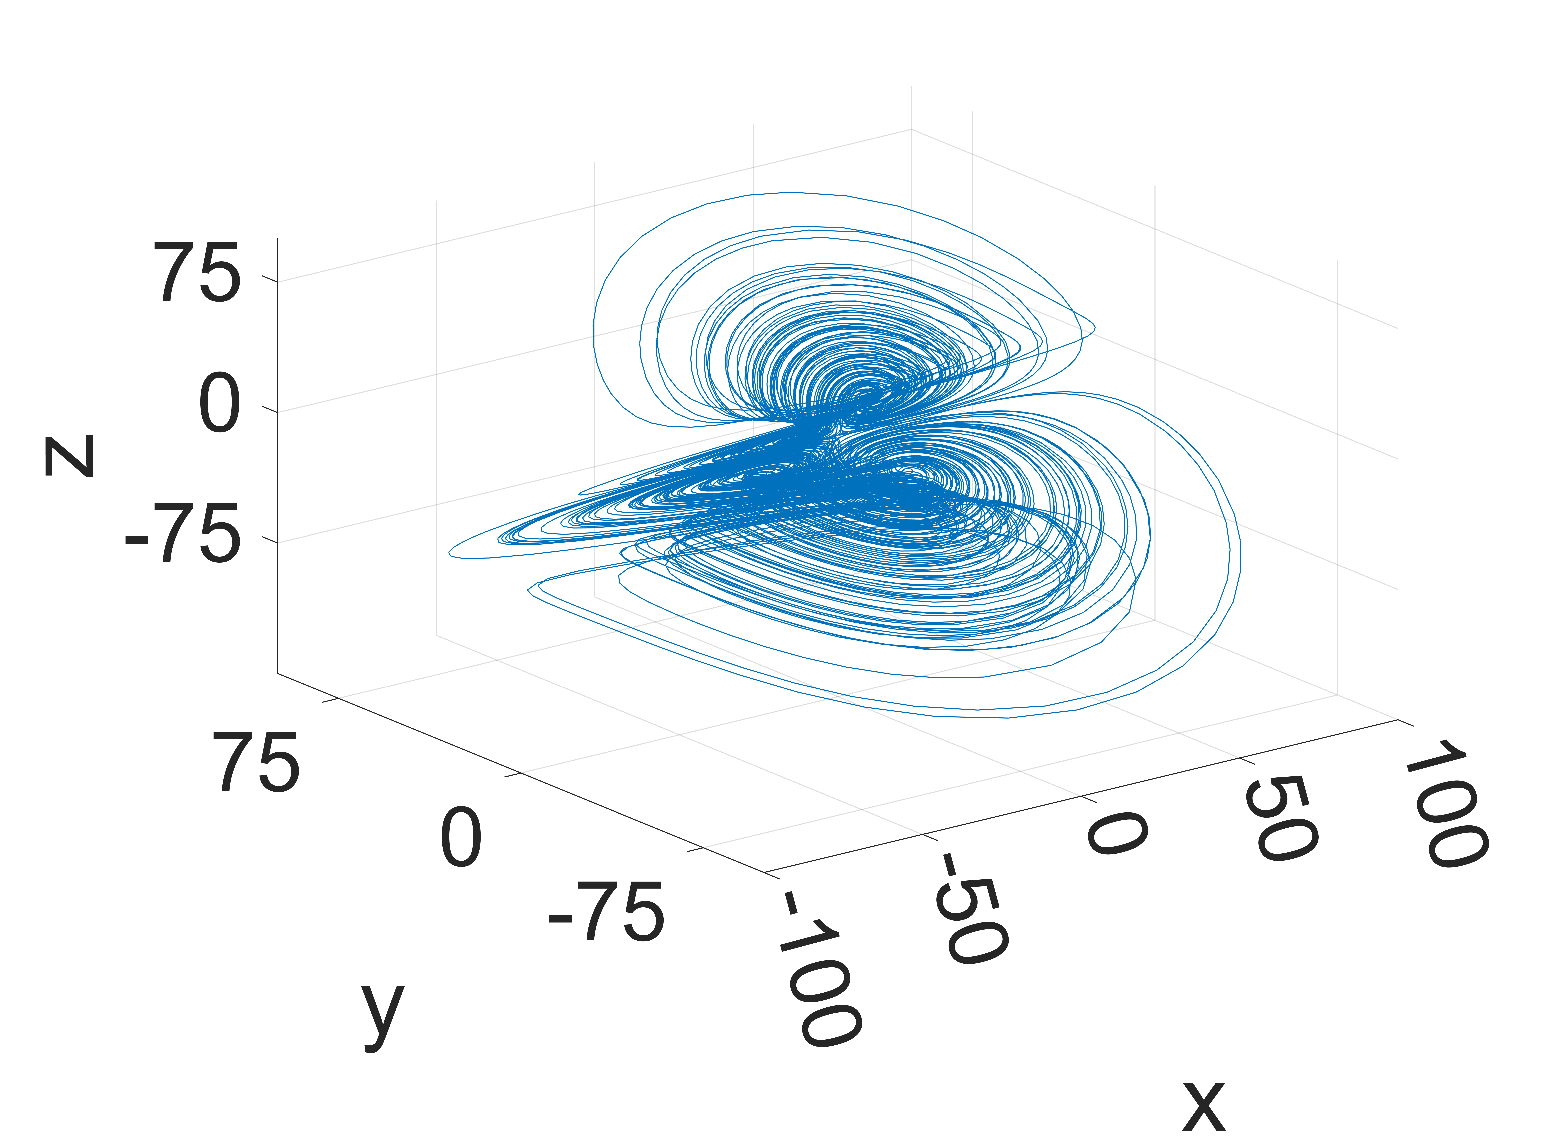
\includegraphics[width=\linewidth]{Figuras IEEE/atractores_4D_HC4S/a.pdf}
    \caption{}
\end{subfigure}
\hfill
\begin{subfigure}{0.48\textwidth}
    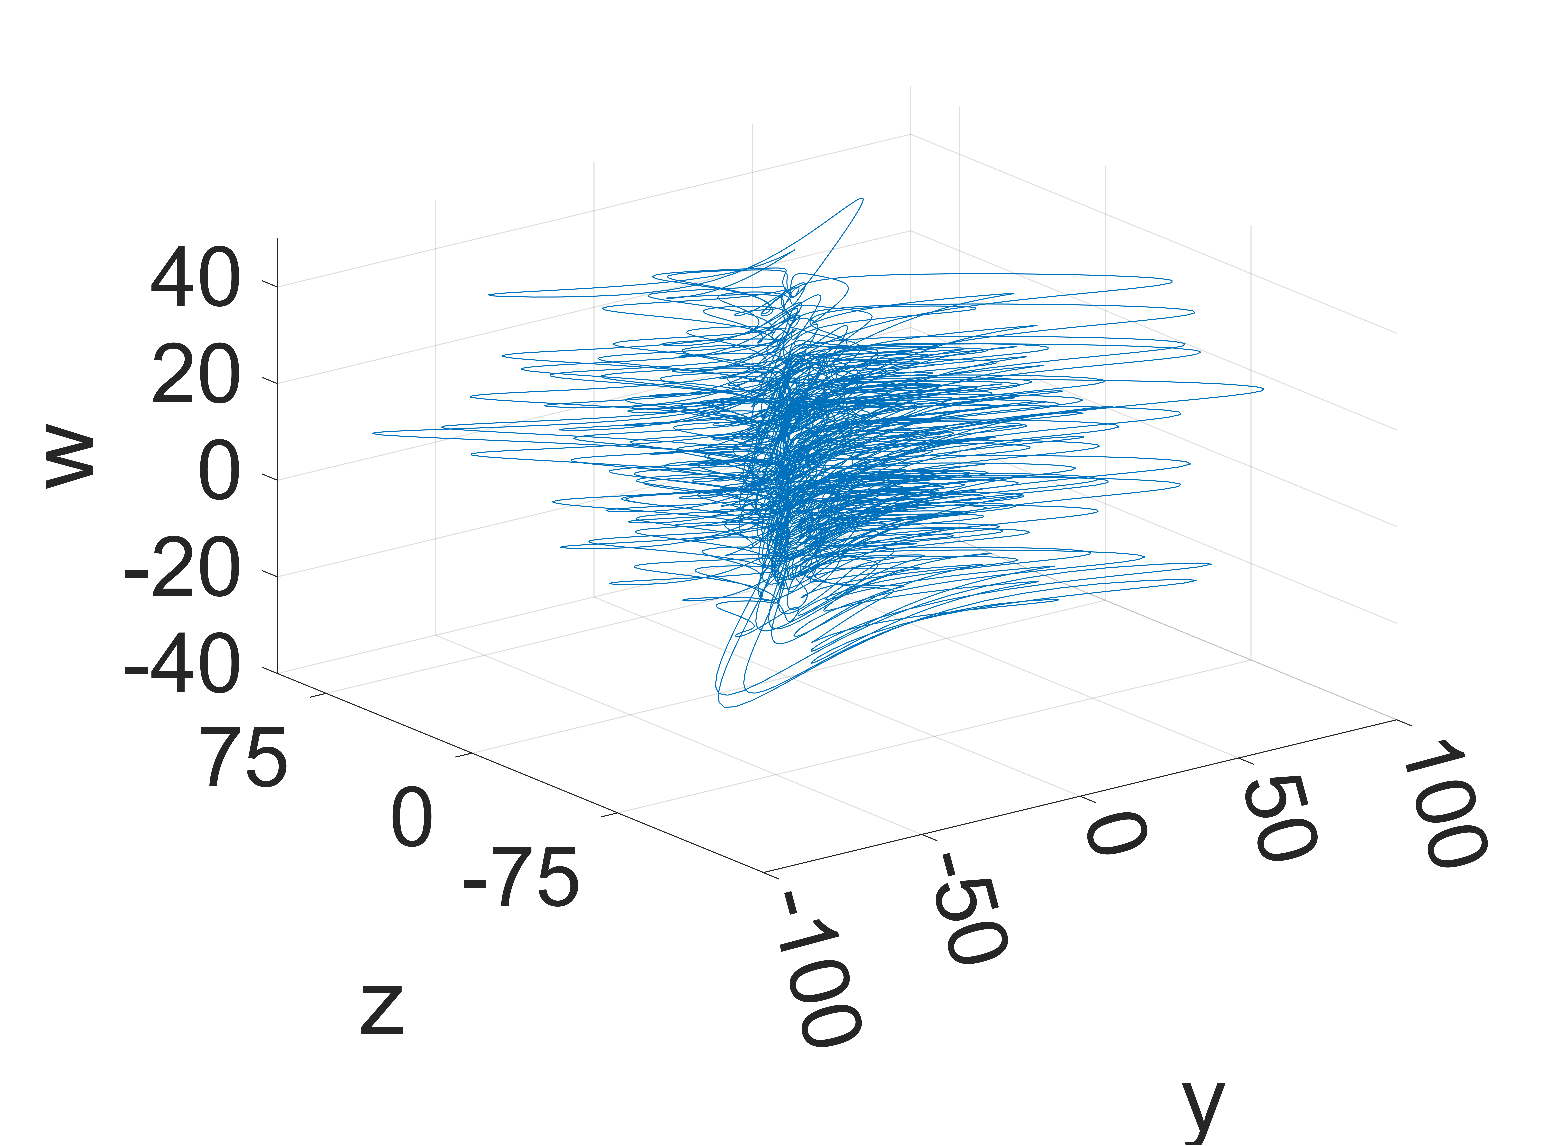
\includegraphics[width=\linewidth]{Figuras IEEE/atractores_4D_HC4S/b.pdf}
    \caption{}
\end{subfigure}

\begin{subfigure}{0.48\textwidth}
    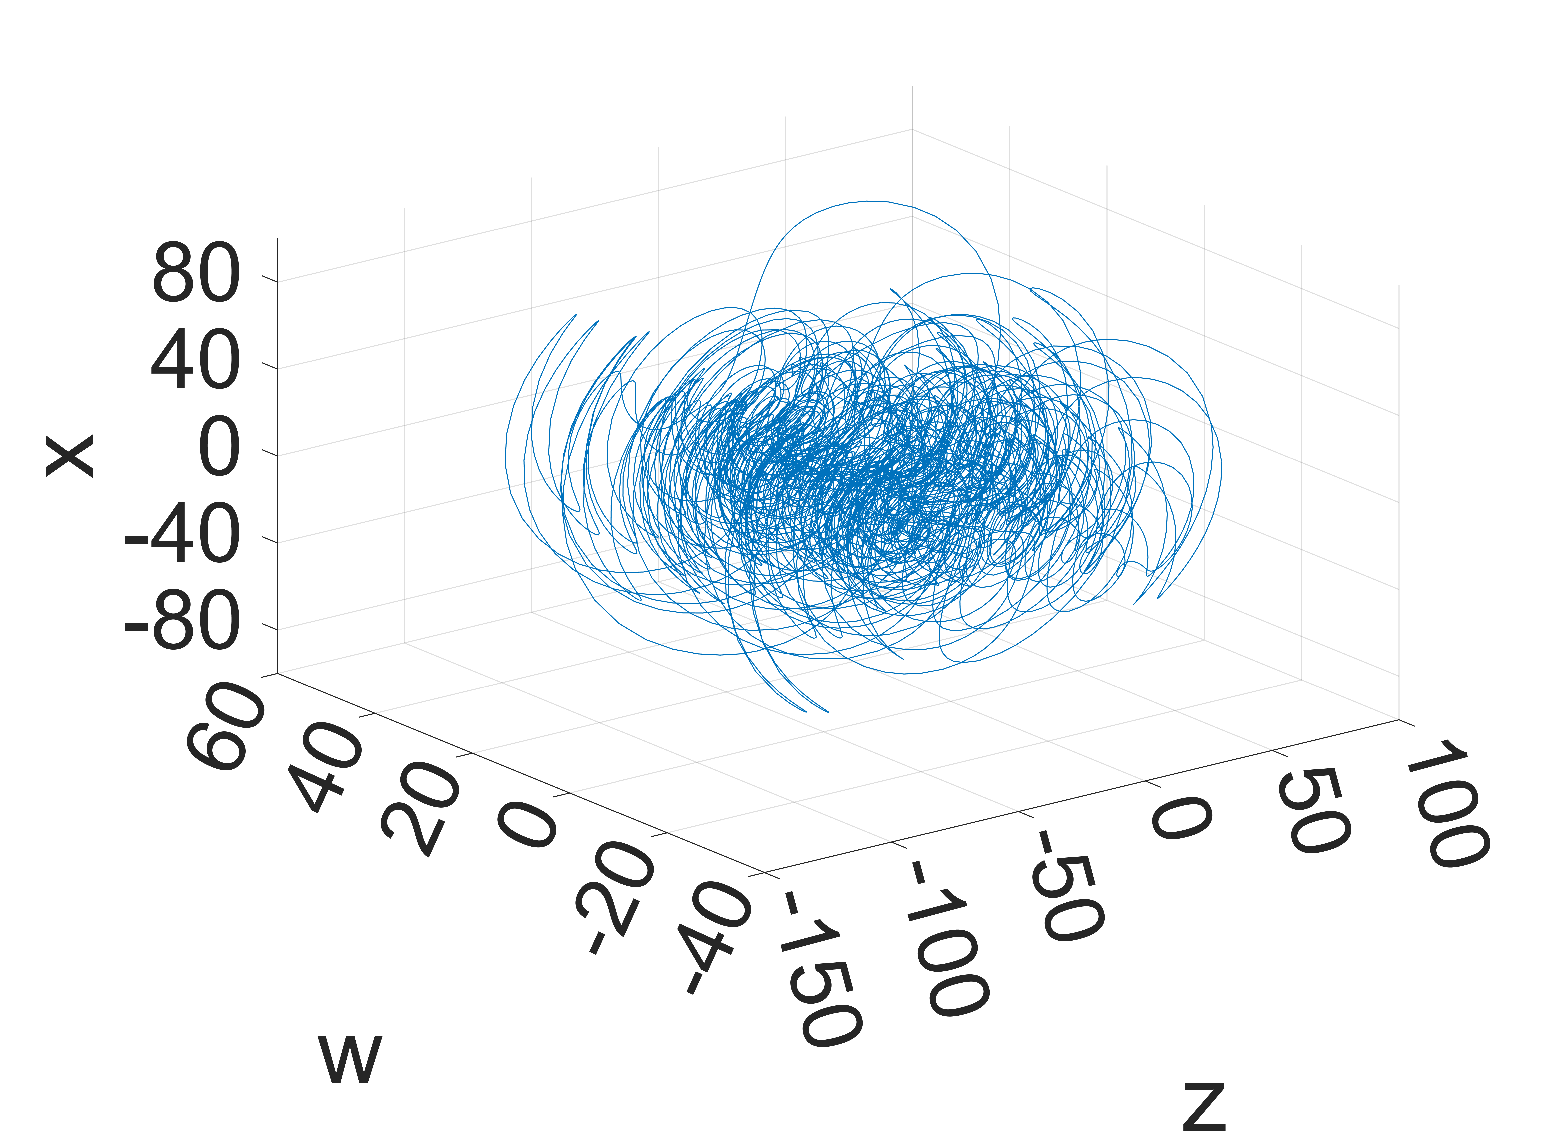
\includegraphics[width=\linewidth]{Figuras IEEE/atractores_4D_HC4S/c.pdf}
    \caption{}
\end{subfigure}
\hfill
\begin{subfigure}{0.48\textwidth}
    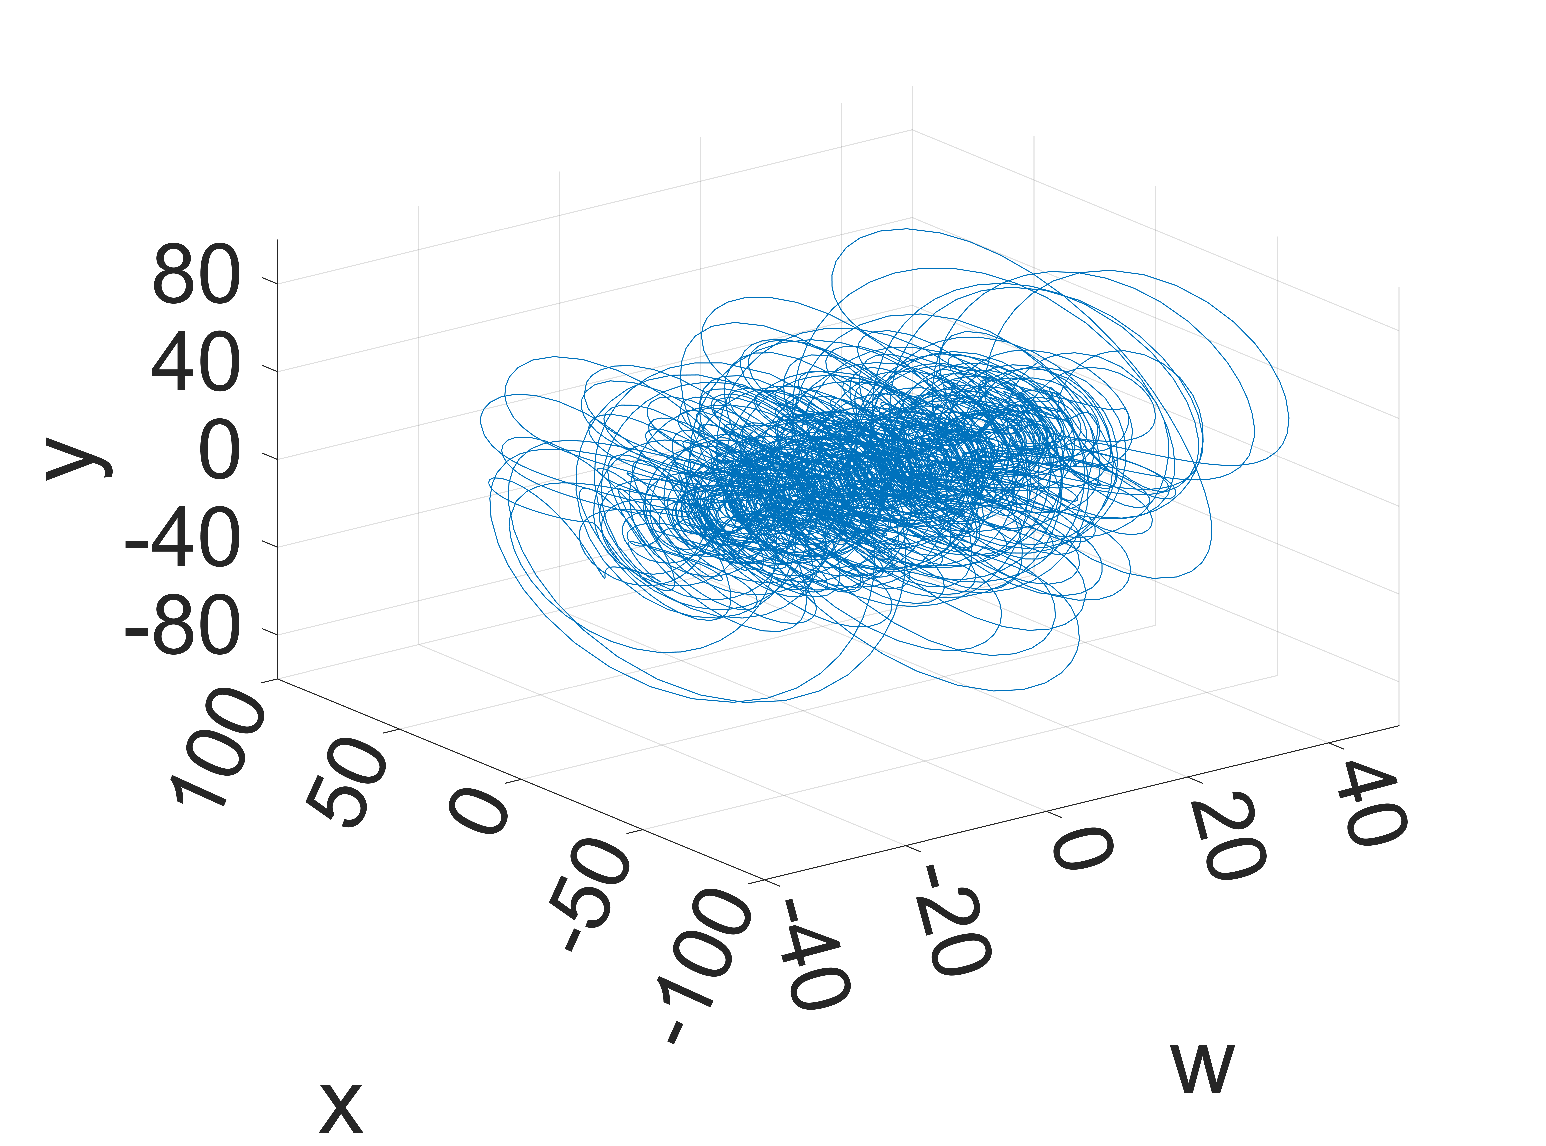
\includegraphics[width=\linewidth]{Figuras IEEE/atractores_4D_HC4S/d.pdf}
    \caption{}
\end{subfigure}

\caption{4D-HC4S phase space diagram. (a) $(x, y, z)$ projection. (b) $(y, z, w)$ projection. (c) $(z, w, x)$ projection. (d) $(w, x, y)$ projection.}
\label{fig_1}
\end{figure*}
Given the parameters $ParX = (9,27,8,0.1)^T$ and the initial conditions $X(0)=(0.3,0.2,0.2,0.3)^T$, its calculated LEs are $LE_1=3.5213$, $LE_2=0.03880$, $LE_3=0.02153$ and $LE_4=-29.54$, which confirms the hyperchaotic nature of the system. 

Using the Benettin algorithm for LE \cite{benettin_lyapunov_1980}, the Lyapunov exponent spectrum was calculated, which confirms that the 4D-HC4S system remains hyperchaotic across wide parameter ranges: $a_{4D}\in[3.8,10]$, $b_{4D}\in[19.3,30]$, $c_{4D}\in[3.1,11.6]$, and $d_{4D}\in[-0.1,1.2]$.

Complementing this, bifurcation diagrams, Figure \ref{fig_3}, visually illustrate the system states' transition from periodic and quasi-periodic states to the desired chaotic regime, corroborating the findings from the spectrum analysis. 

\begin{figure*}[!t]
\centering
\begin{subfigure}{0.48\textwidth}
    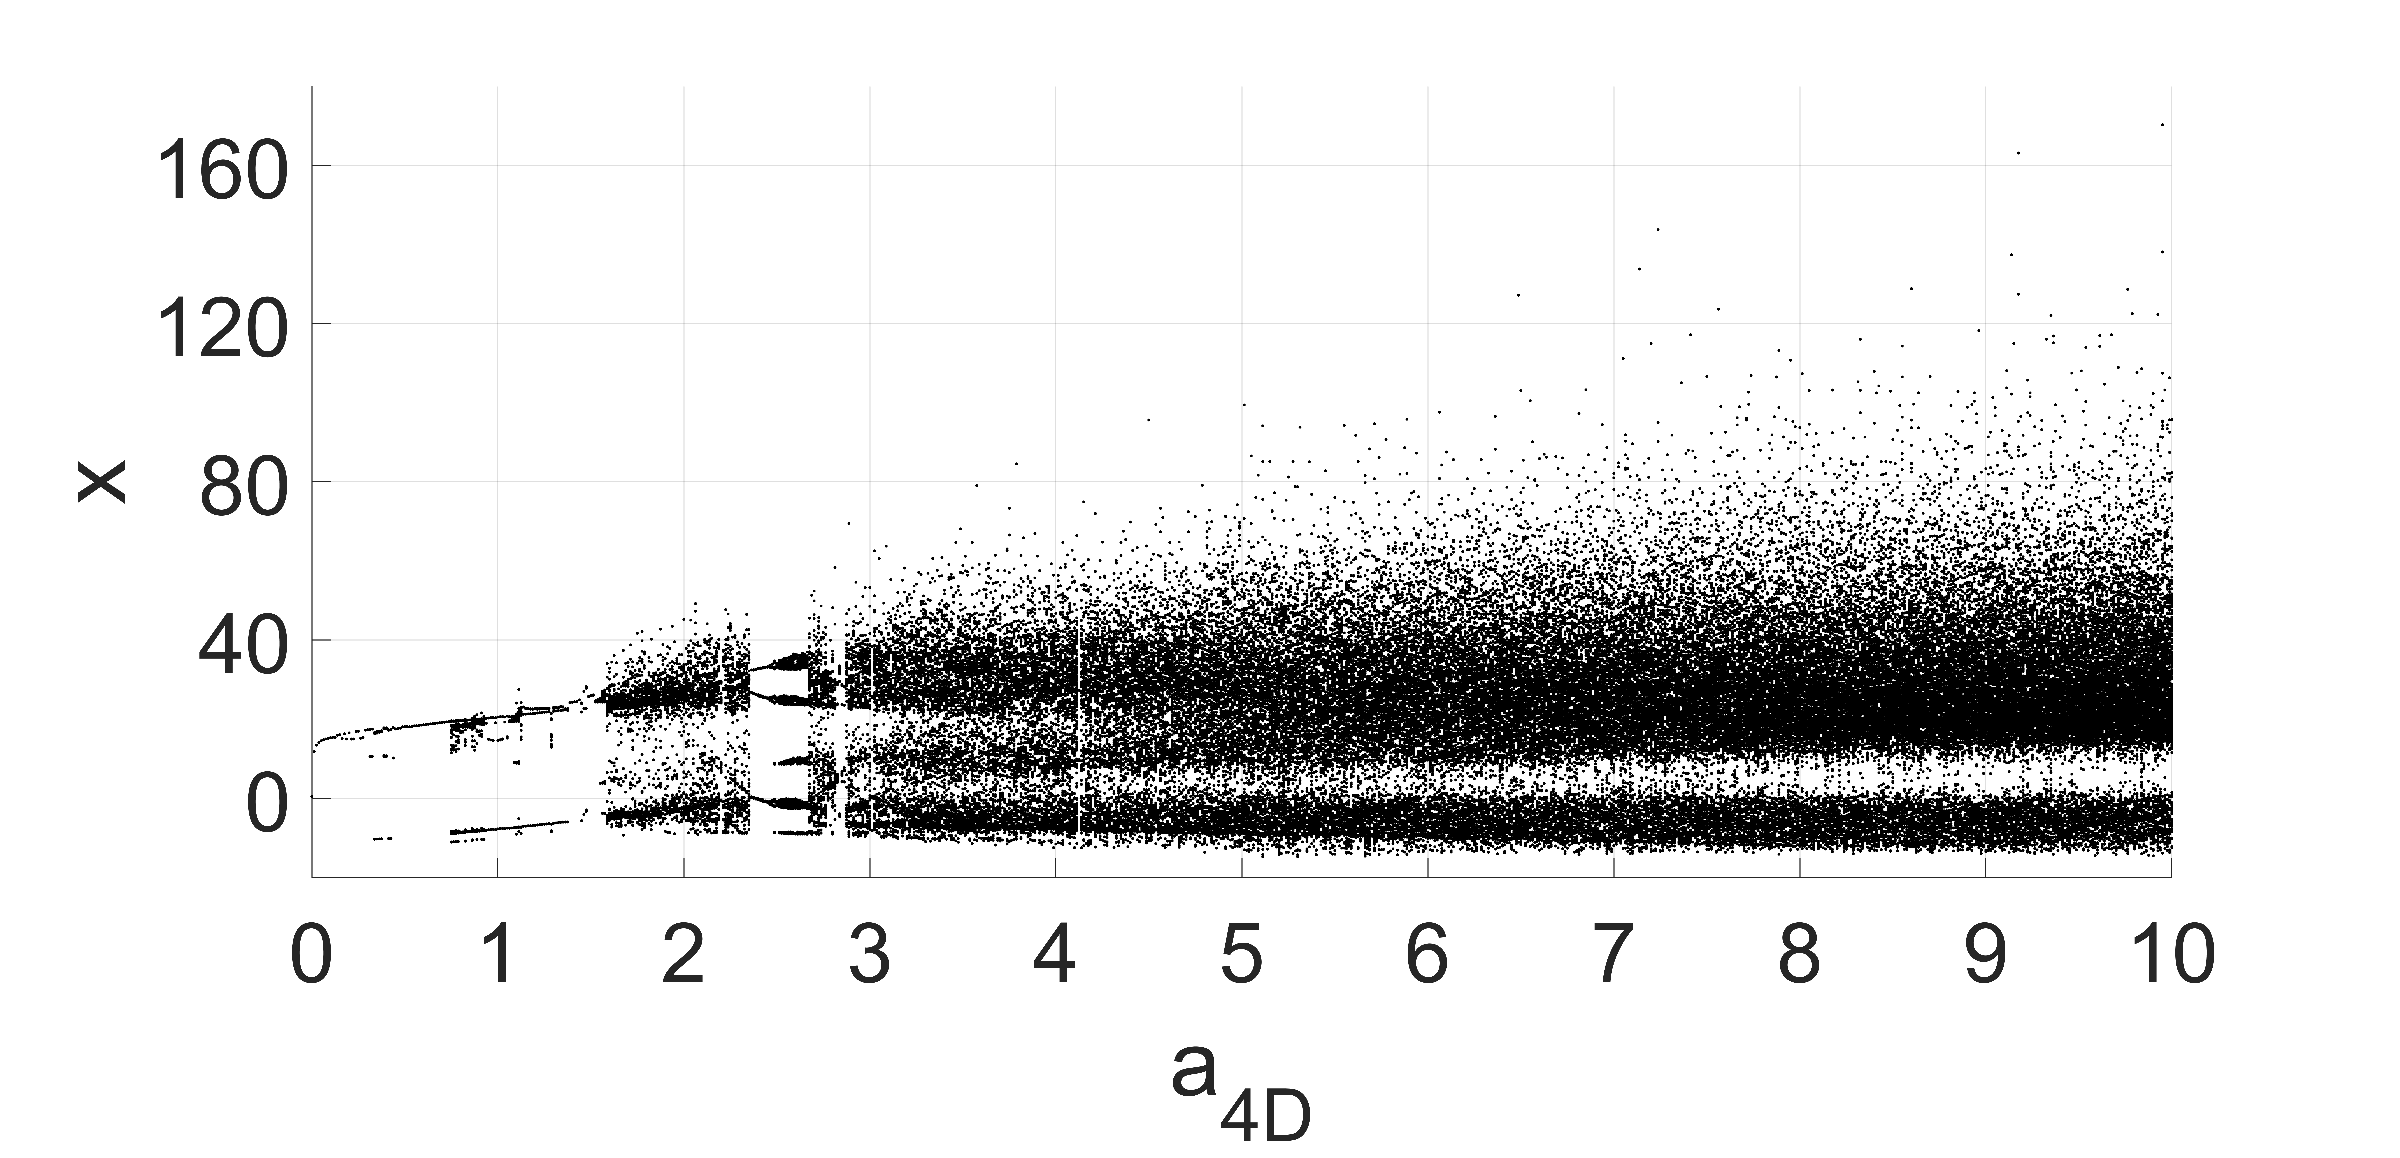
\includegraphics[width=\linewidth]{Figuras IEEE/bifurcation_4D_HC4S/a.pdf}
    \caption{}
\end{subfigure}
\hfill
\begin{subfigure}{0.48\textwidth}
    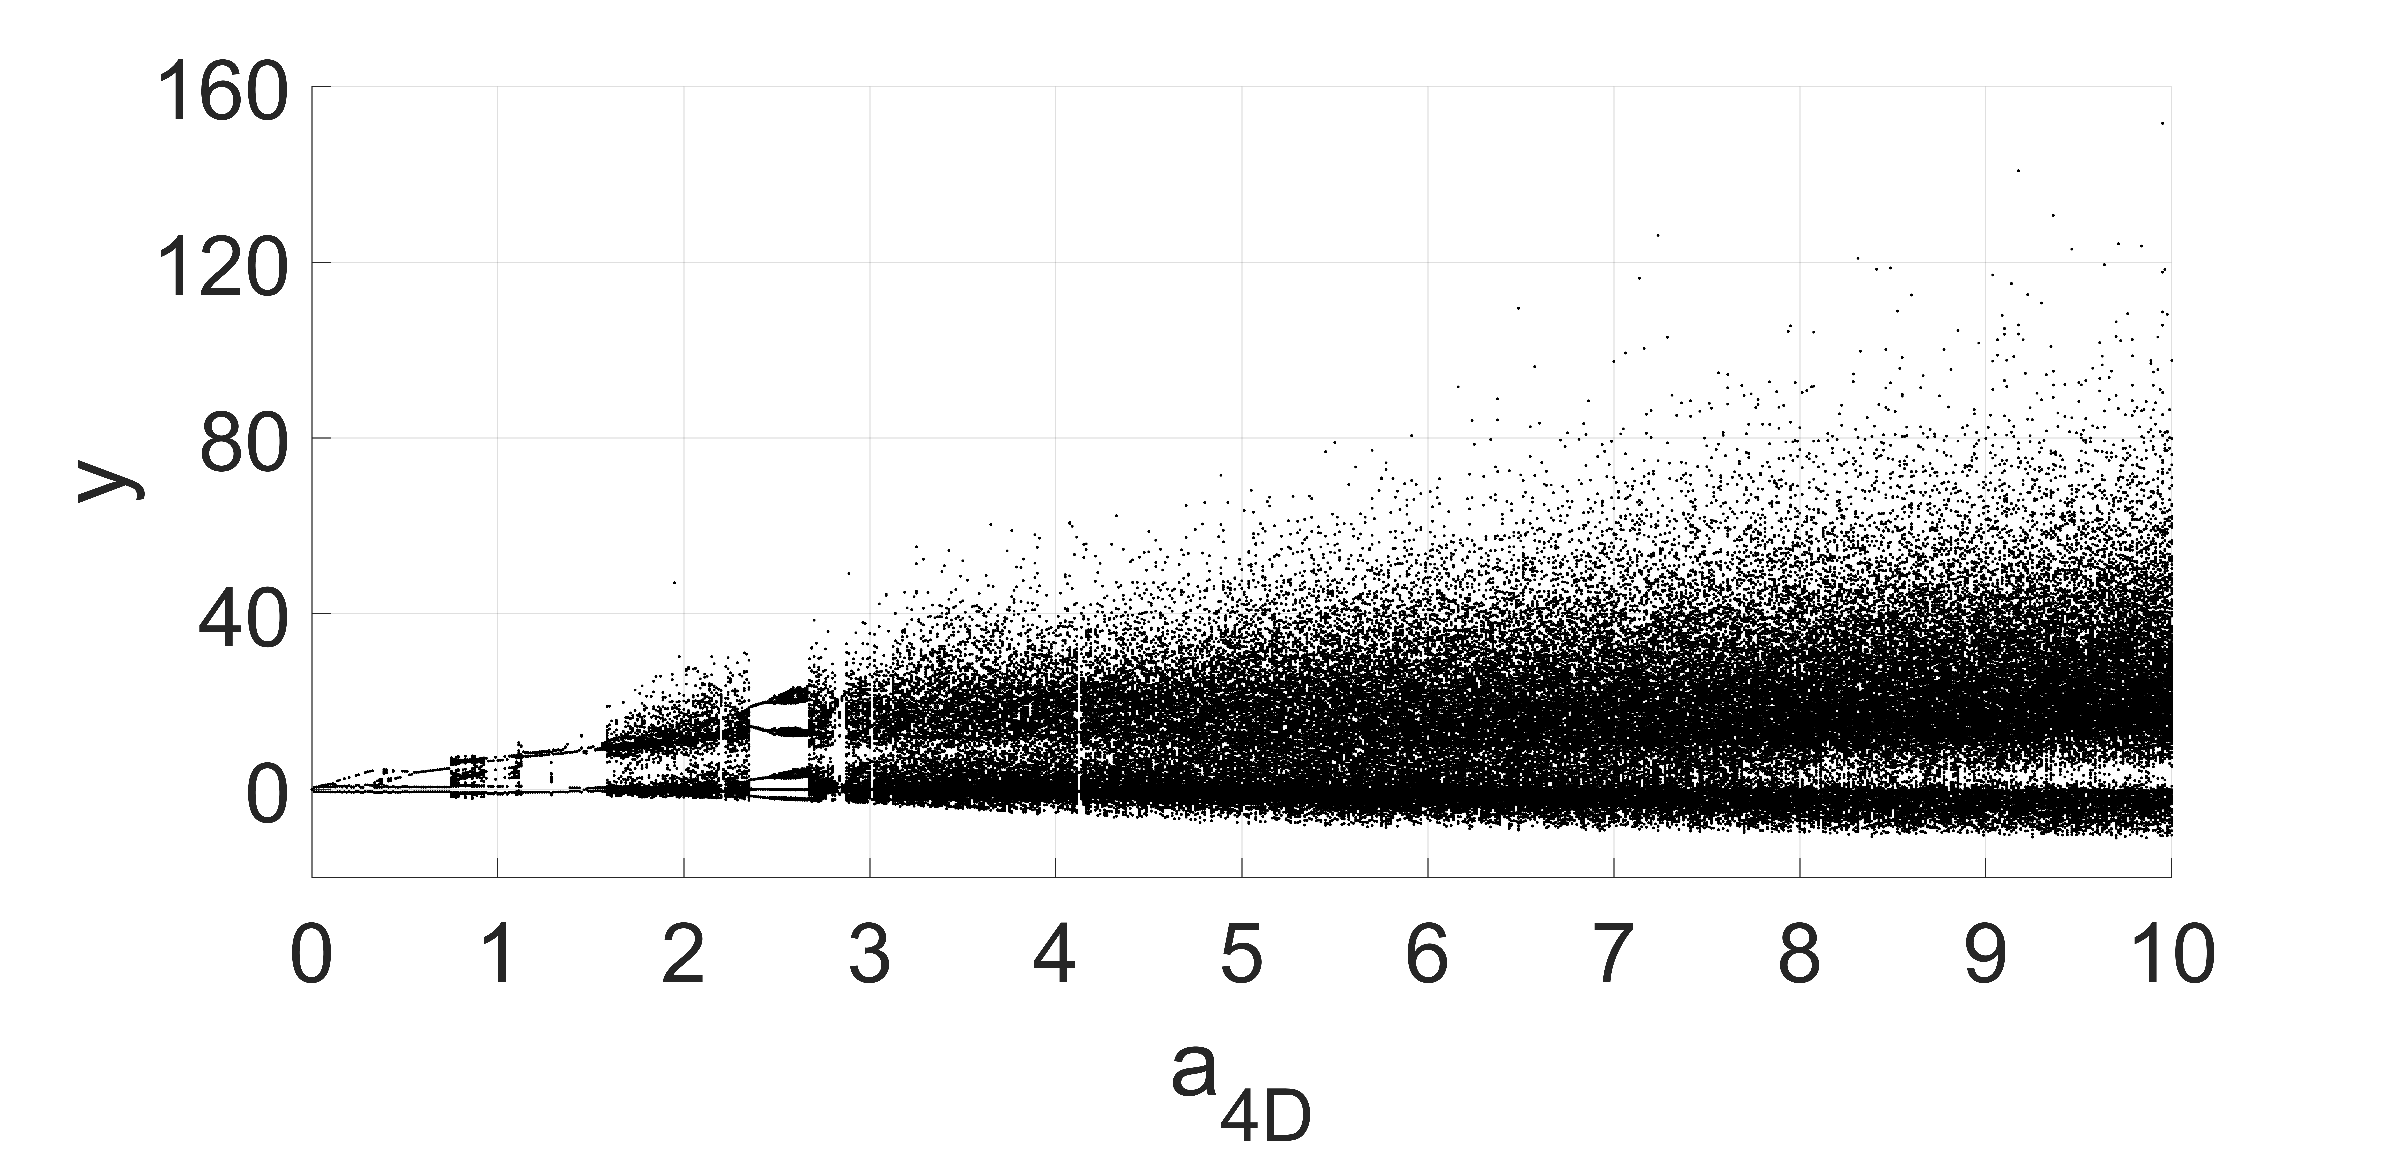
\includegraphics[width=\linewidth]{Figuras IEEE/bifurcation_4D_HC4S/b.pdf}
    \caption{}
\end{subfigure}

\begin{subfigure}{0.48\textwidth}
    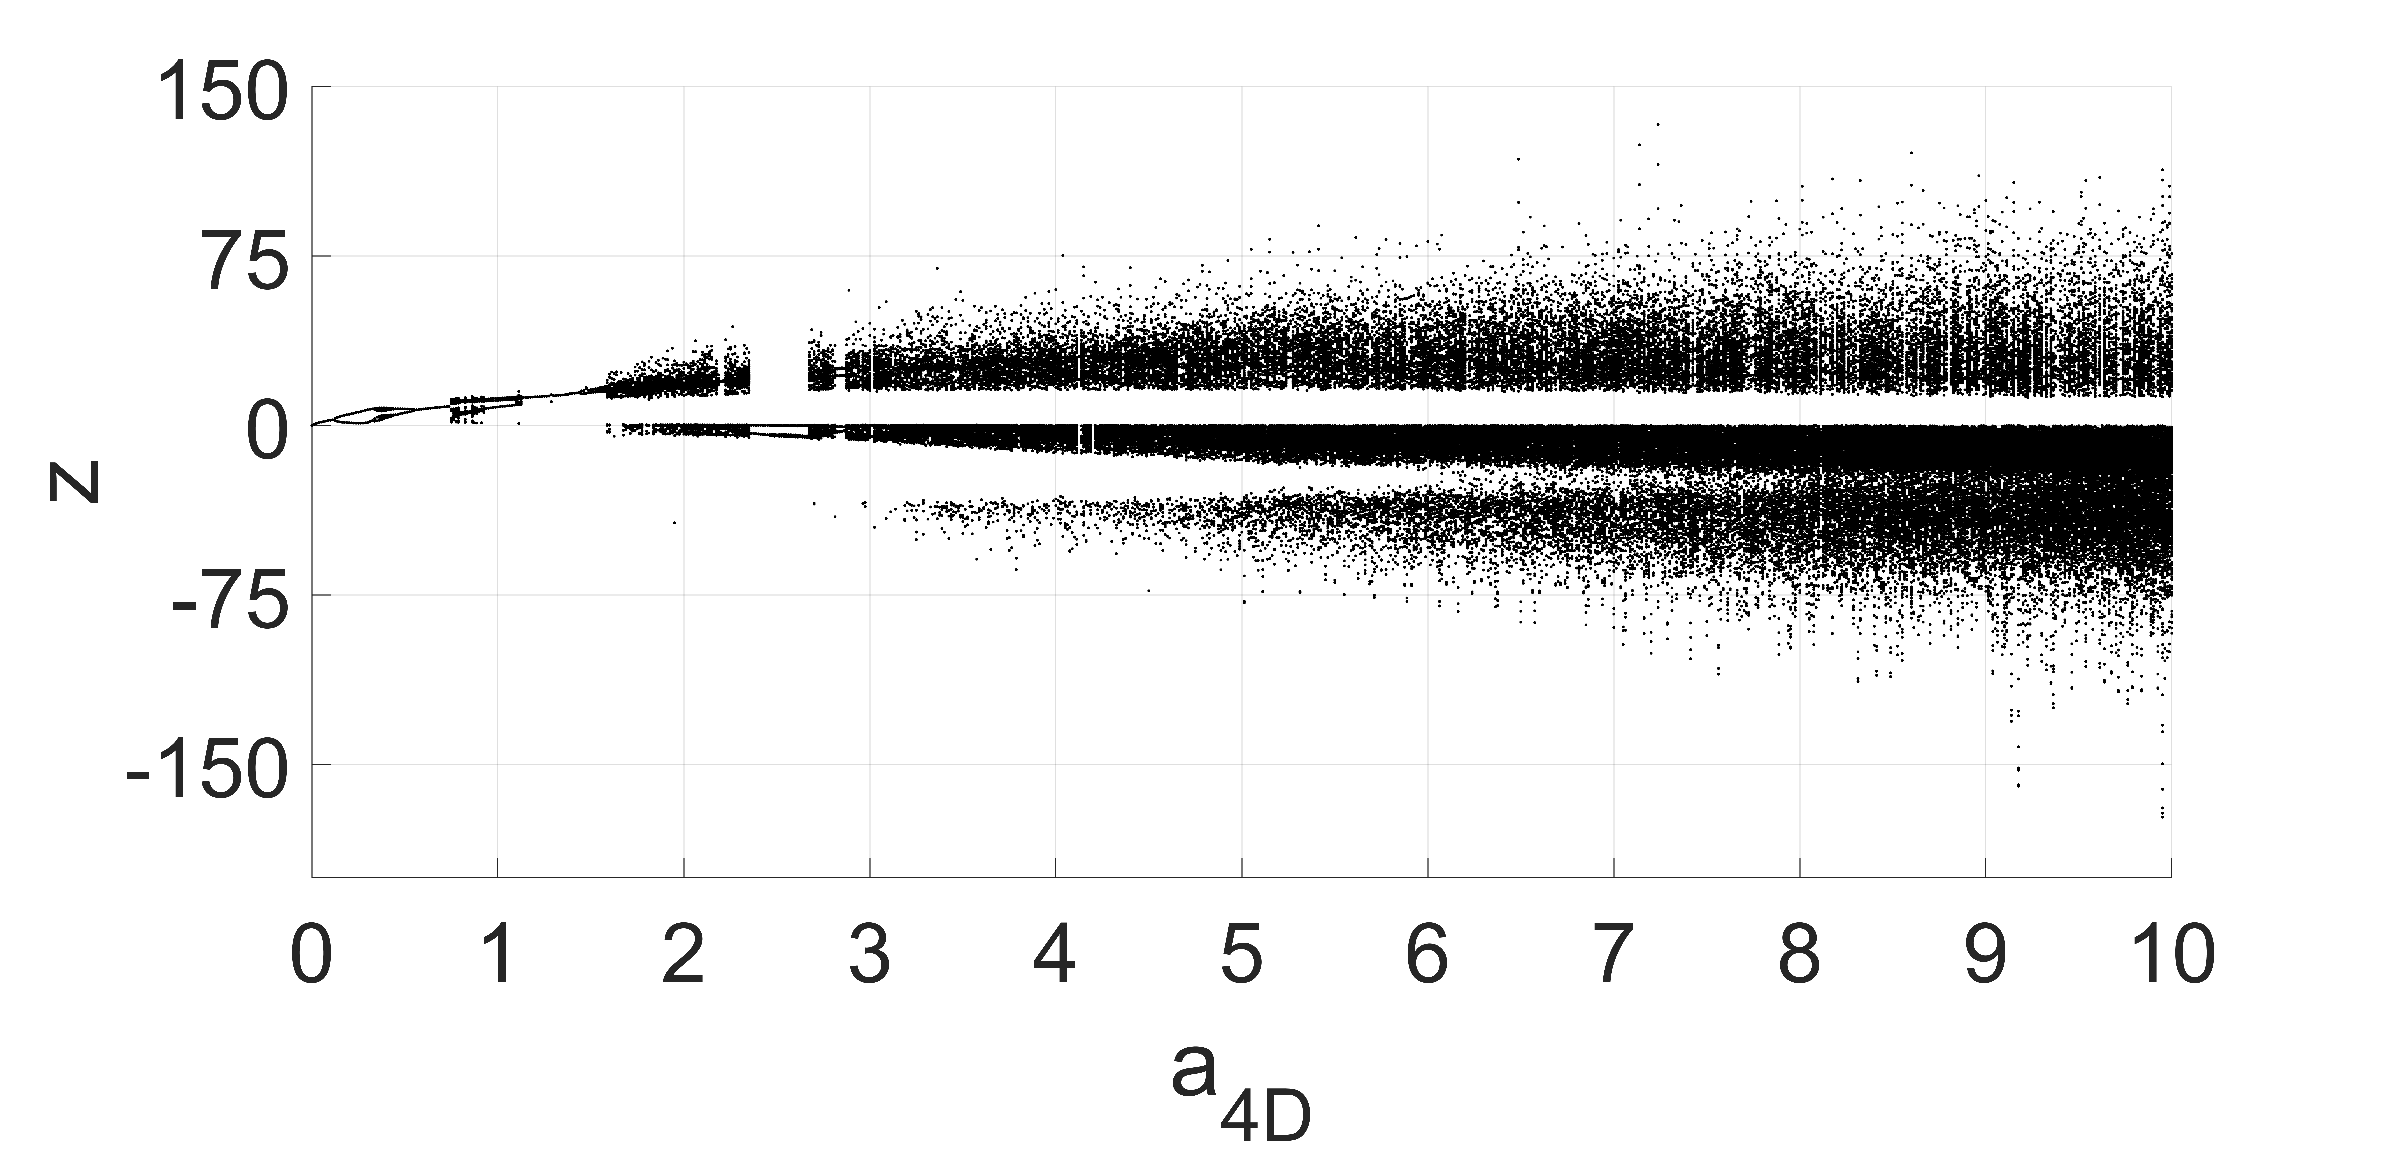
\includegraphics[width=\linewidth]{Figuras IEEE/bifurcation_4D_HC4S/c.pdf}
    \caption{}
\end{subfigure}
\hfill
\begin{subfigure}{0.48\textwidth}
    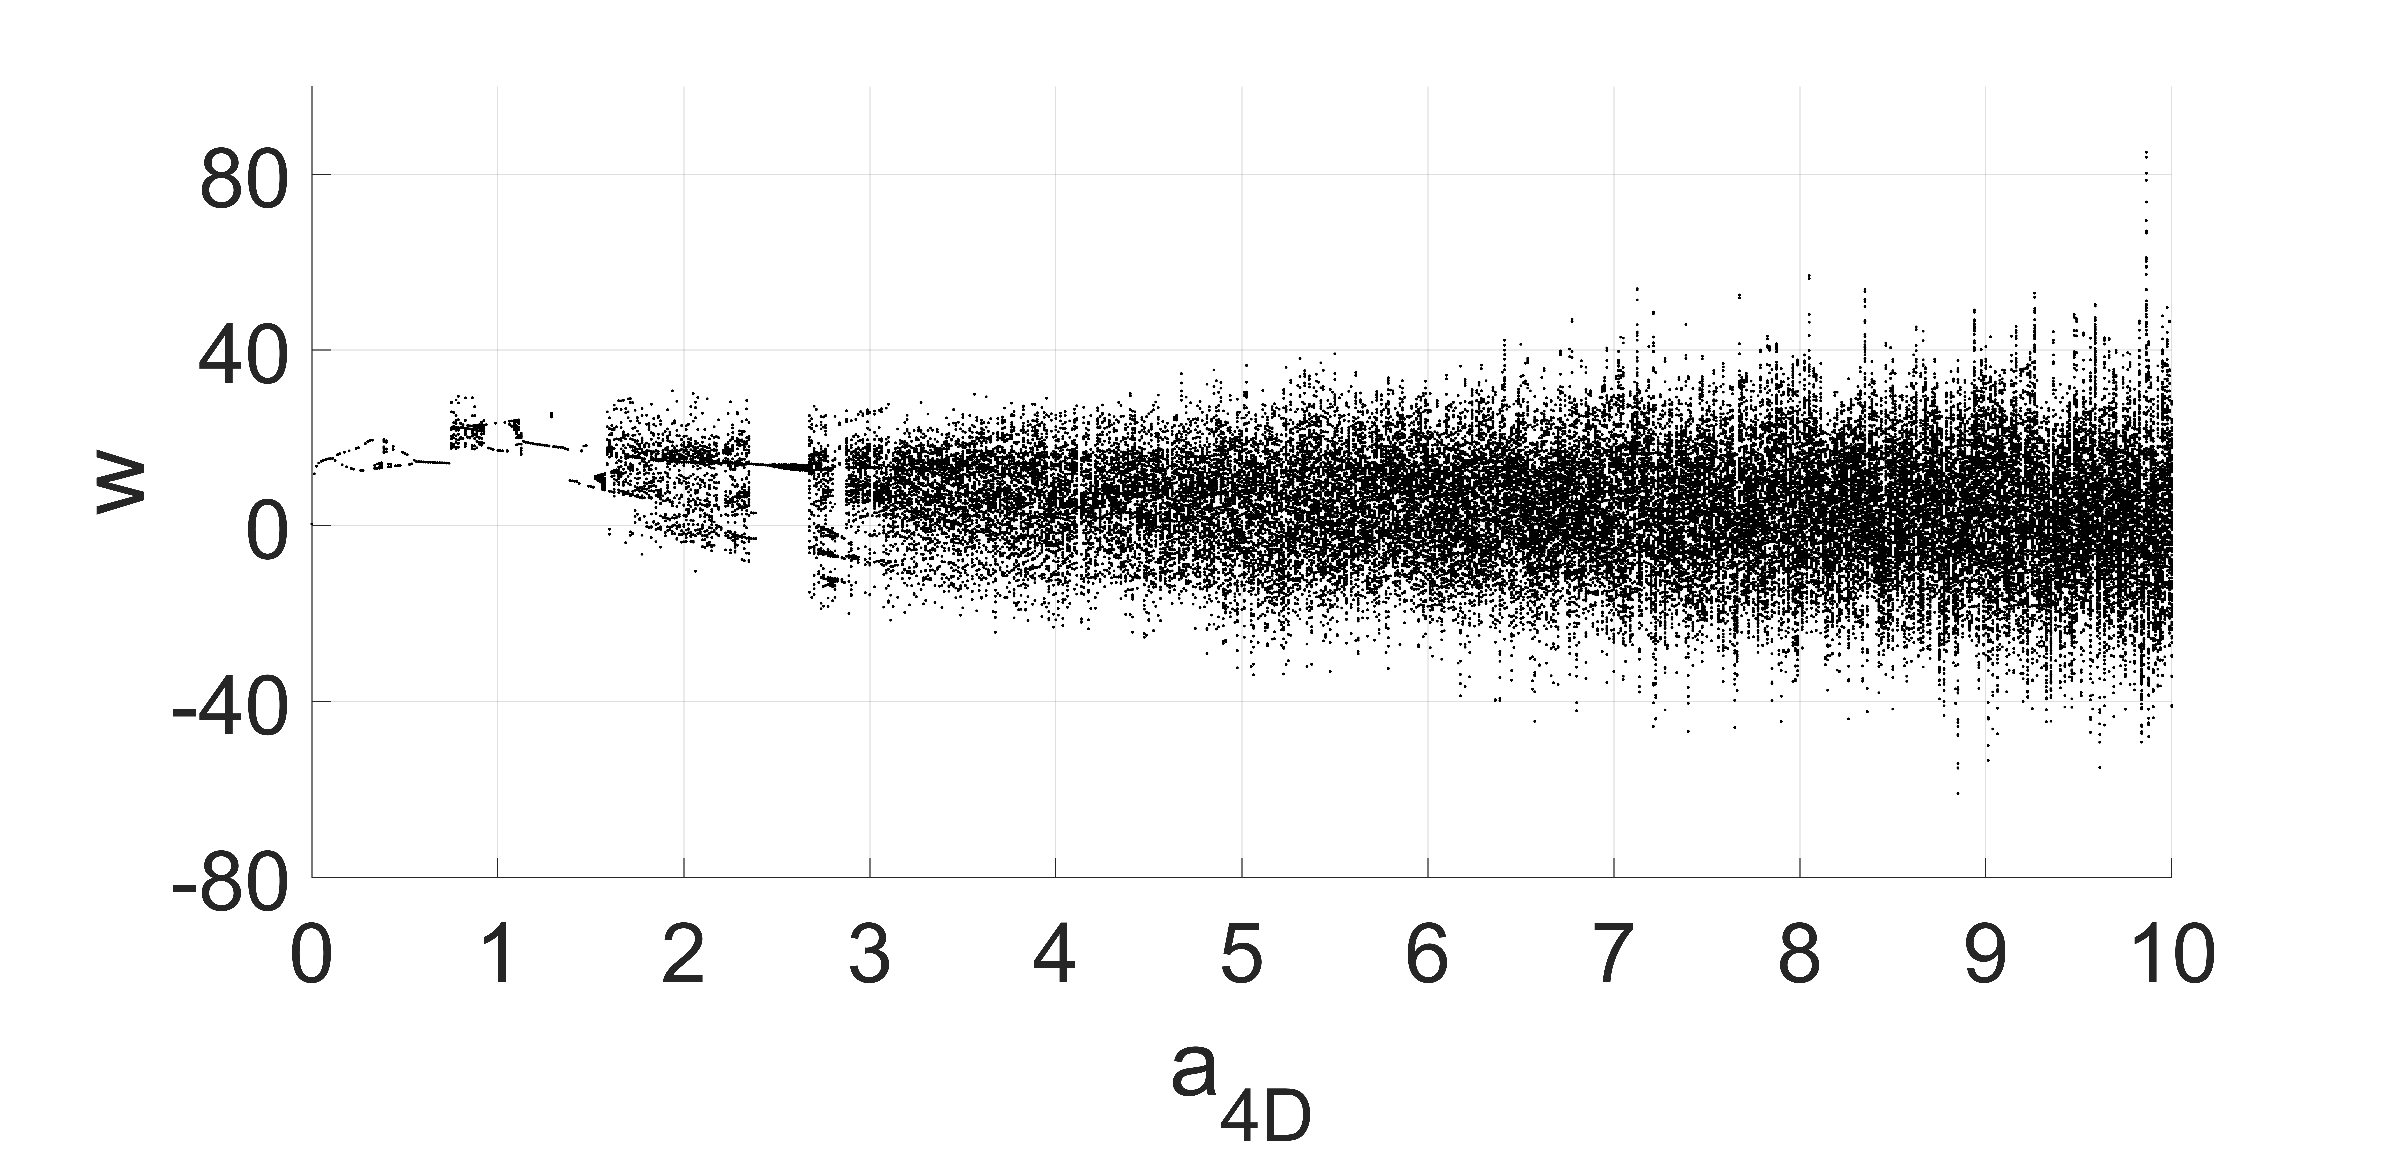
\includegraphics[width=\linewidth]{Figuras IEEE/bifurcation_4D_HC4S/d.pdf}
    \caption{}
\end{subfigure}

\caption{The 4D-HC4S bifurcation diagram as a $a_{4D}$ parameter sweep. (a) $x$ state. (b) $y$ state. (c) $z$ state. (d) $w$ state.}
\label{fig_3}
\end{figure*}
For digital implementation, the continuous system is discretized using the efficient and simple Euler method, since it offers lower computational cost per iteration than more resource intensive Runge–Kutta methods.
To accurately capture the hyperchaotic behavior,without causing chaotic degradation while minimizing the number of iterations needed in the system, a time difference of $h=0.0001$ is used, higher values resulted in the chaotic behavior degrating. This application of Euler’s method to 4D-HC4S results in Eq. \ref{eq_2}.
\begin{equation}
\begin{split}
 X_{n+1} &= X_n+h({\text{4D-HC4S}}(X_n, ParX))\\
&= {\text{Eu-4D}}(X_n, ParX)
\end{split}
\label{eq_2}
\end{equation}
%% Use \subsection commands to start a subsection.

\subsection{Proposed enhanced 4D hyperchaotic four-scroll system}
\label{subsec3_2}
The introduction of modular multiplication has been shown to improve the chaotic characteristics of a system, particularly its sensitivity to initial conditions \cite{hua_two-dimensional_2020, meranza-castillon_pseudorandom_2019, murillo-escobar_pseudorandom_2023}. This principle is applied to the 4D-HC4S system by multiplying its states by a large number, 12227, and then applying a modulo 1 operation to extract the fractional component. This constant was selected empirically based on its ability to produce a mostly uniform distribution across the state space, while being large enough to allow proper mixing of smaller and higher decimals.

Applying this enhancement to the original 4D-HC4S discretized system (Eq. \ref{eq_2}), the 4D Enhanced Hyperchaotic Four-Scroll System (4D-EHC4S) was created and is described in Eq. \ref{eq_4} and Eq. \ref{eq_5}. This new system will be used as the primary module of the proposed PRNG. Here, $XE$ represents the states of the system, though it uses the same variables, time difference $h$ and set of equations defined in 4D-HC4S. 
\begin{align}
\label{eq_4}
\text{Mod}(x) &= (12227x )  \bmod 1\\
\label{eq_5}
\begin{split}
XE_{n+1} &= \text{Mod}( {\text{Eu-4D}}(XE_n, ParX_n)) \\
         &=   \text{4D-EHC4S}(XE_n, ParX_n)
\end{split}
\end{align}

As can be seen in the bifurcation diagram for this new system Figure \ref{fig_3.5}, the system's sensitivity to initial conditions in its chaotic range is notably enhanced by the modular multiplication. 
This performance gain is a direct result of employing modular multiplication, strengthening chaotic properties, and expanding the range of parameters where chaos occurs.
{\color{red}
The Lyapunov exponents of the discretized system, in nats/iteration, are given by Eq. \ref{eq_EHC4S}.
\begin{align}
\label{eq_EHC4S}
LE &\approx \ln(multiplier) + LE({\text{Eu-4D}})_{cont} \times h
\end{align}
Thus the all the LEs of the system approach 9.4114 in this case. While a higher value of the multiplier or parameters may seem a much better approach, the higher computational cost of using the multipliers needs to be taken into account, more discussion on the parameters selected is given i a future section.
}

\begin{figure*}[!t]
\centering
\subfloat[]{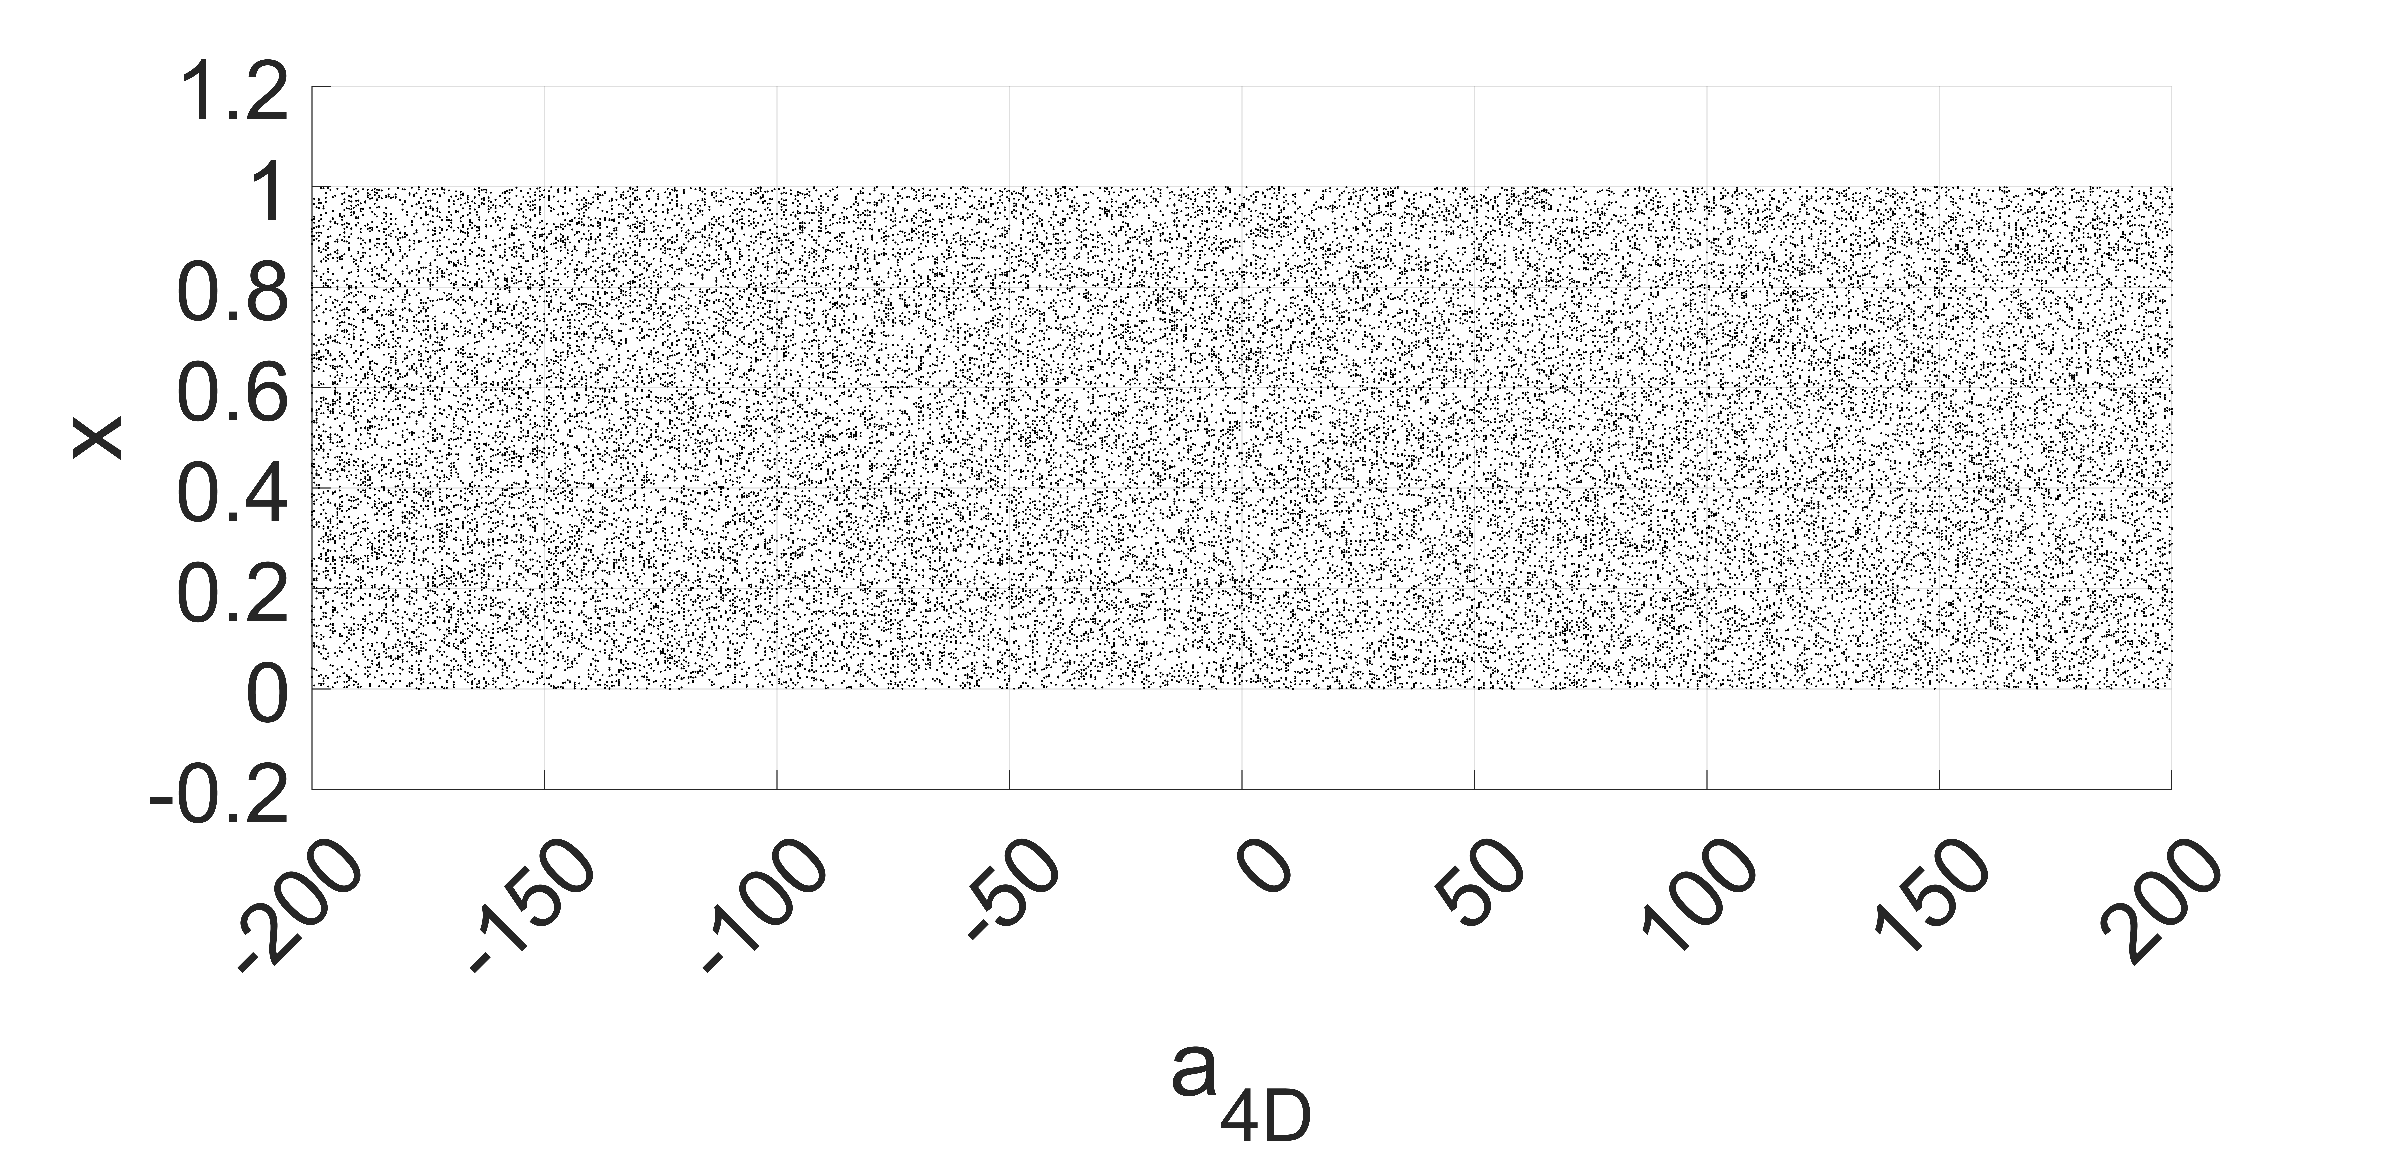
\includegraphics[width=0.48\textwidth]{Figuras IEEE/bifurcation_4D_EHC4S/a.pdf}}% 1
\hfill
\subfloat[]{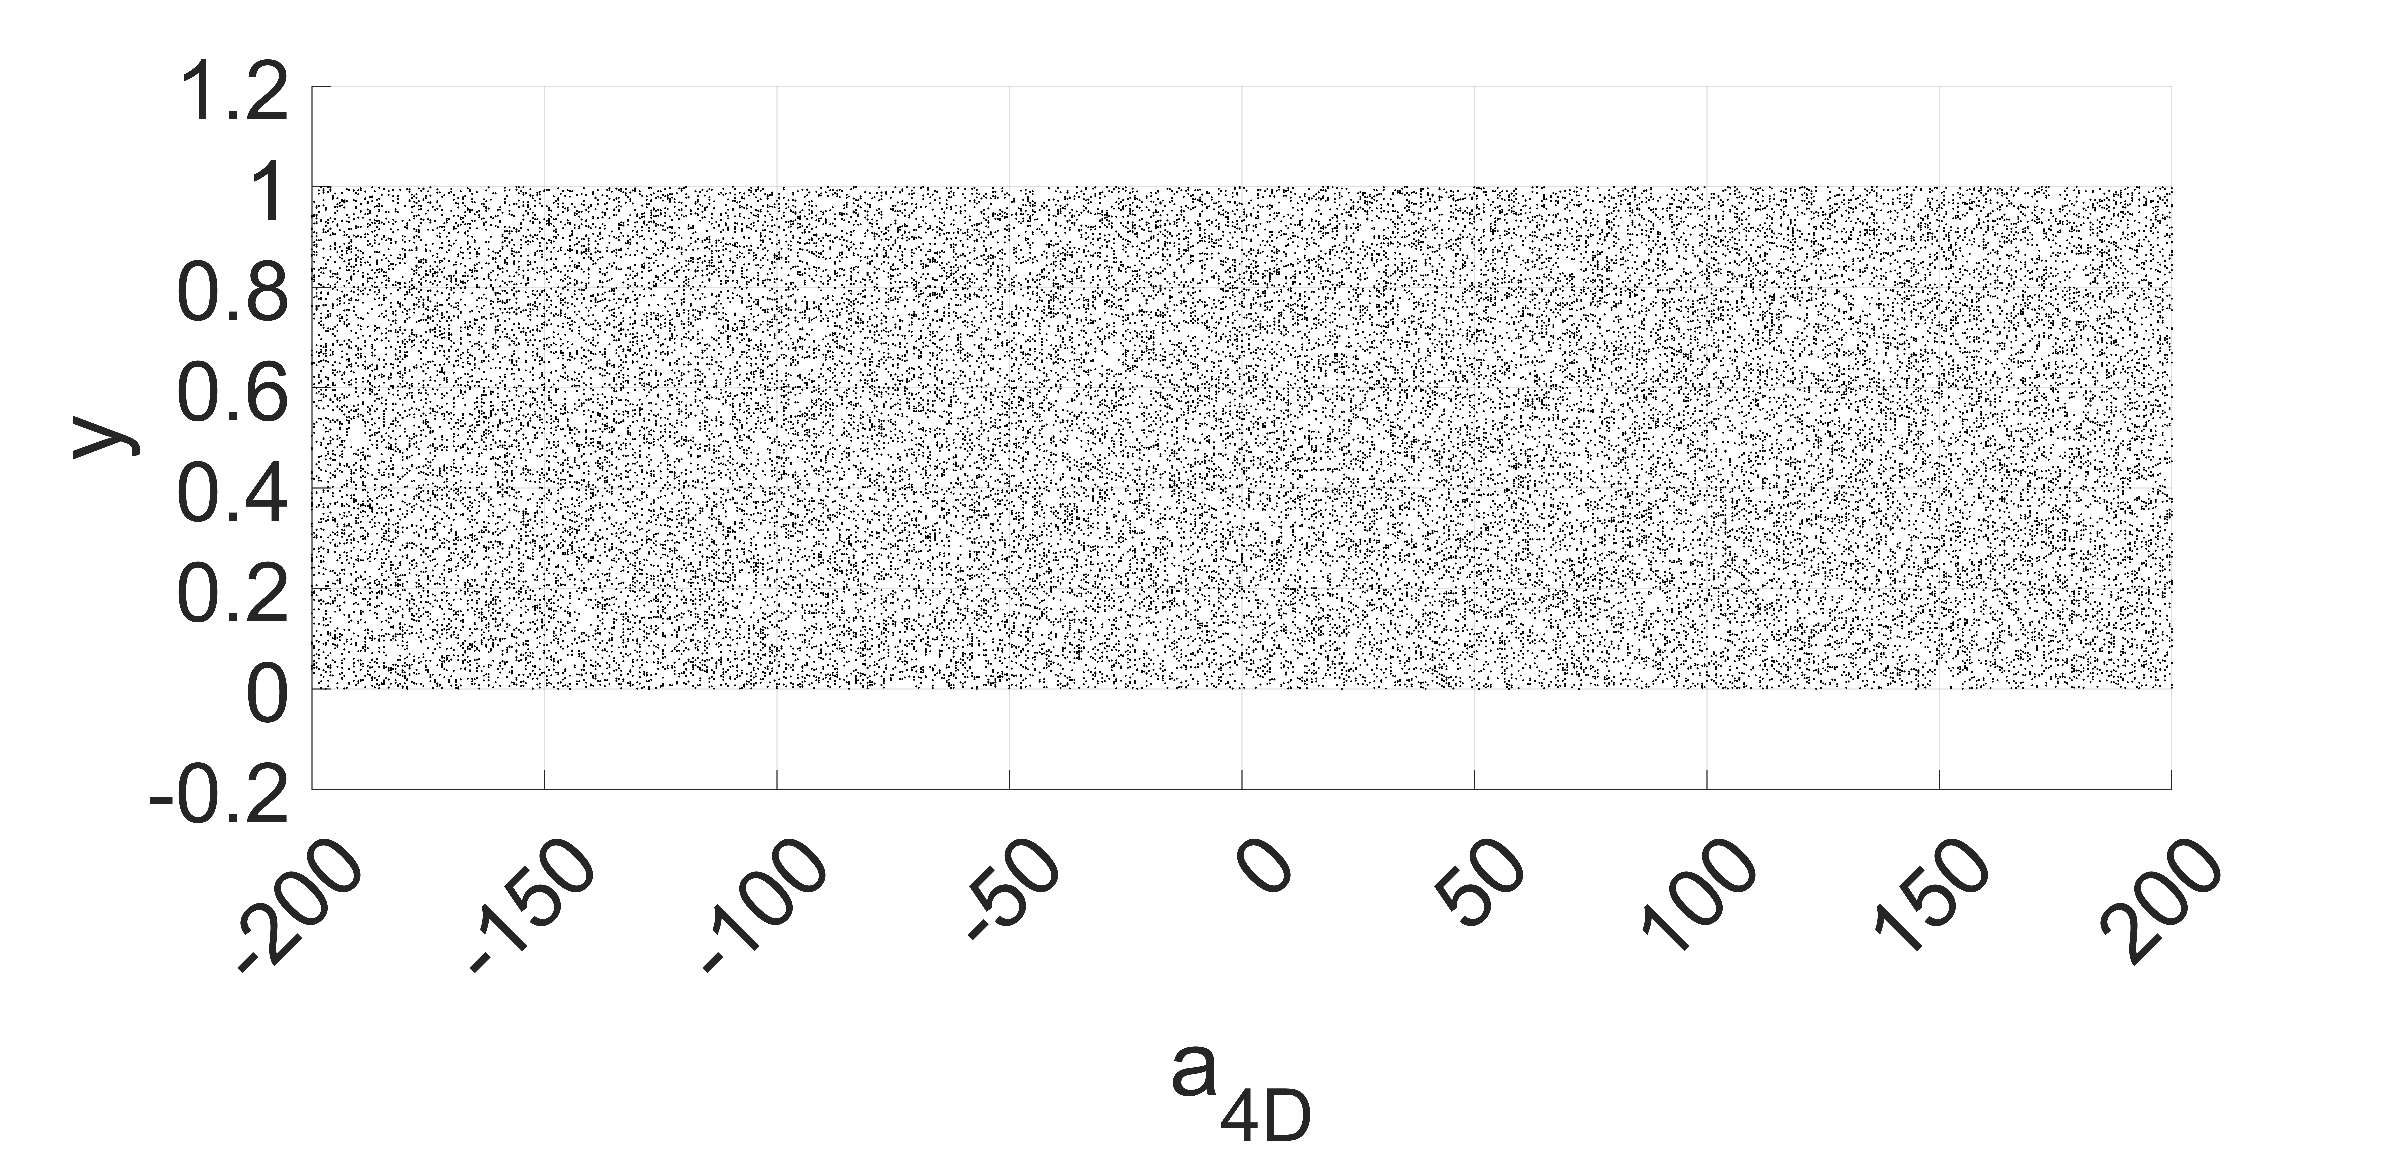
\includegraphics[width=0.48\textwidth]{Figuras IEEE/bifurcation_4D_EHC4S/b.pdf}}% 2

\subfloat[]{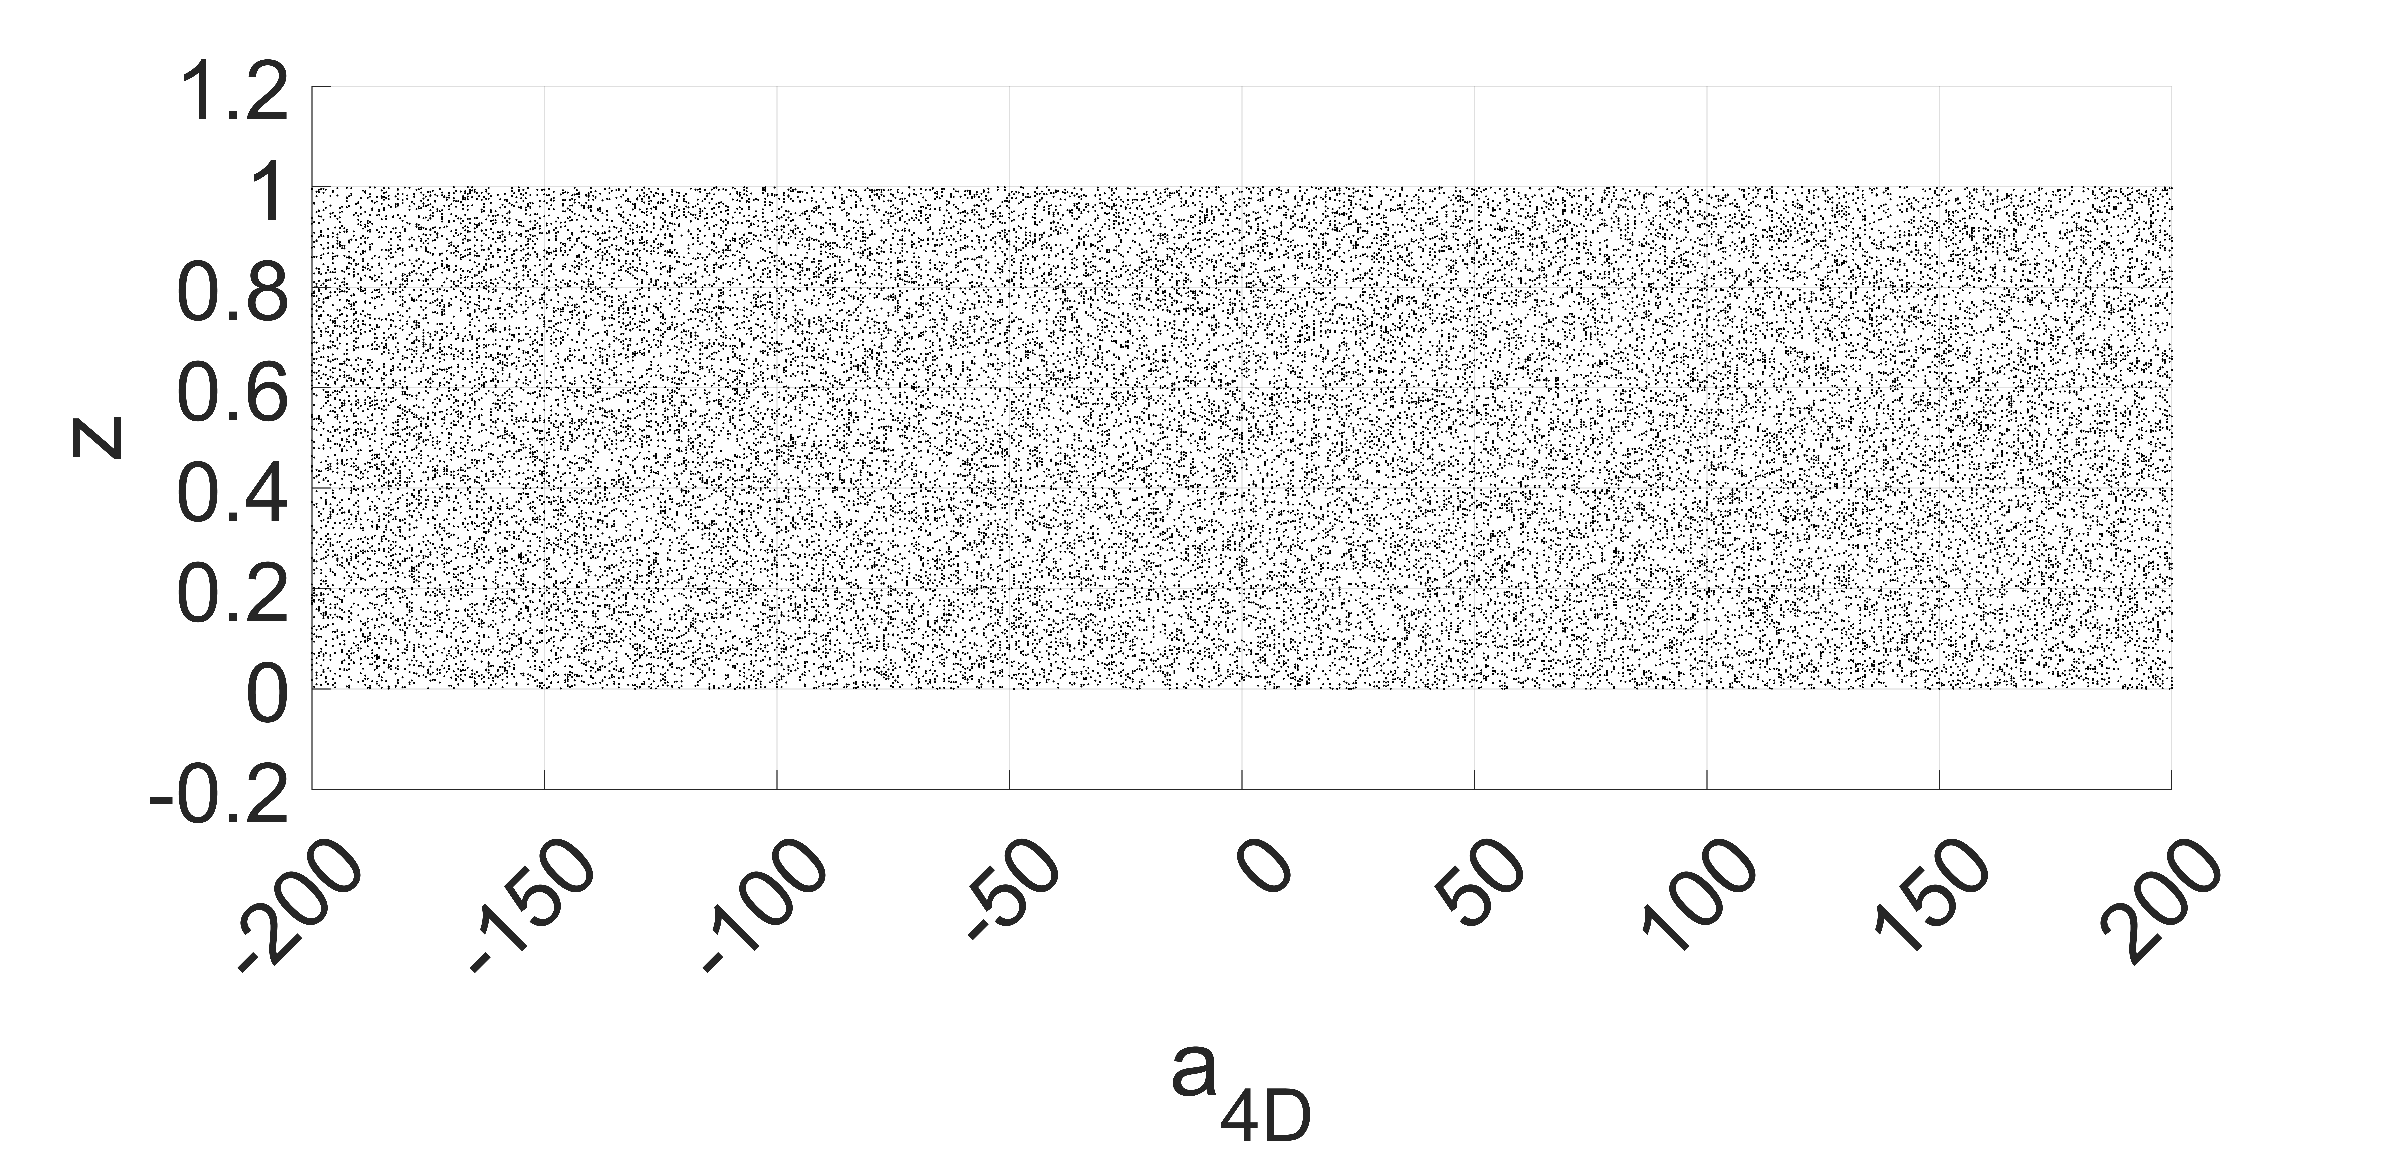
\includegraphics[width=0.48\textwidth]{Figuras IEEE/bifurcation_4D_EHC4S/c.pdf}}% 4
\hfill
\subfloat[]{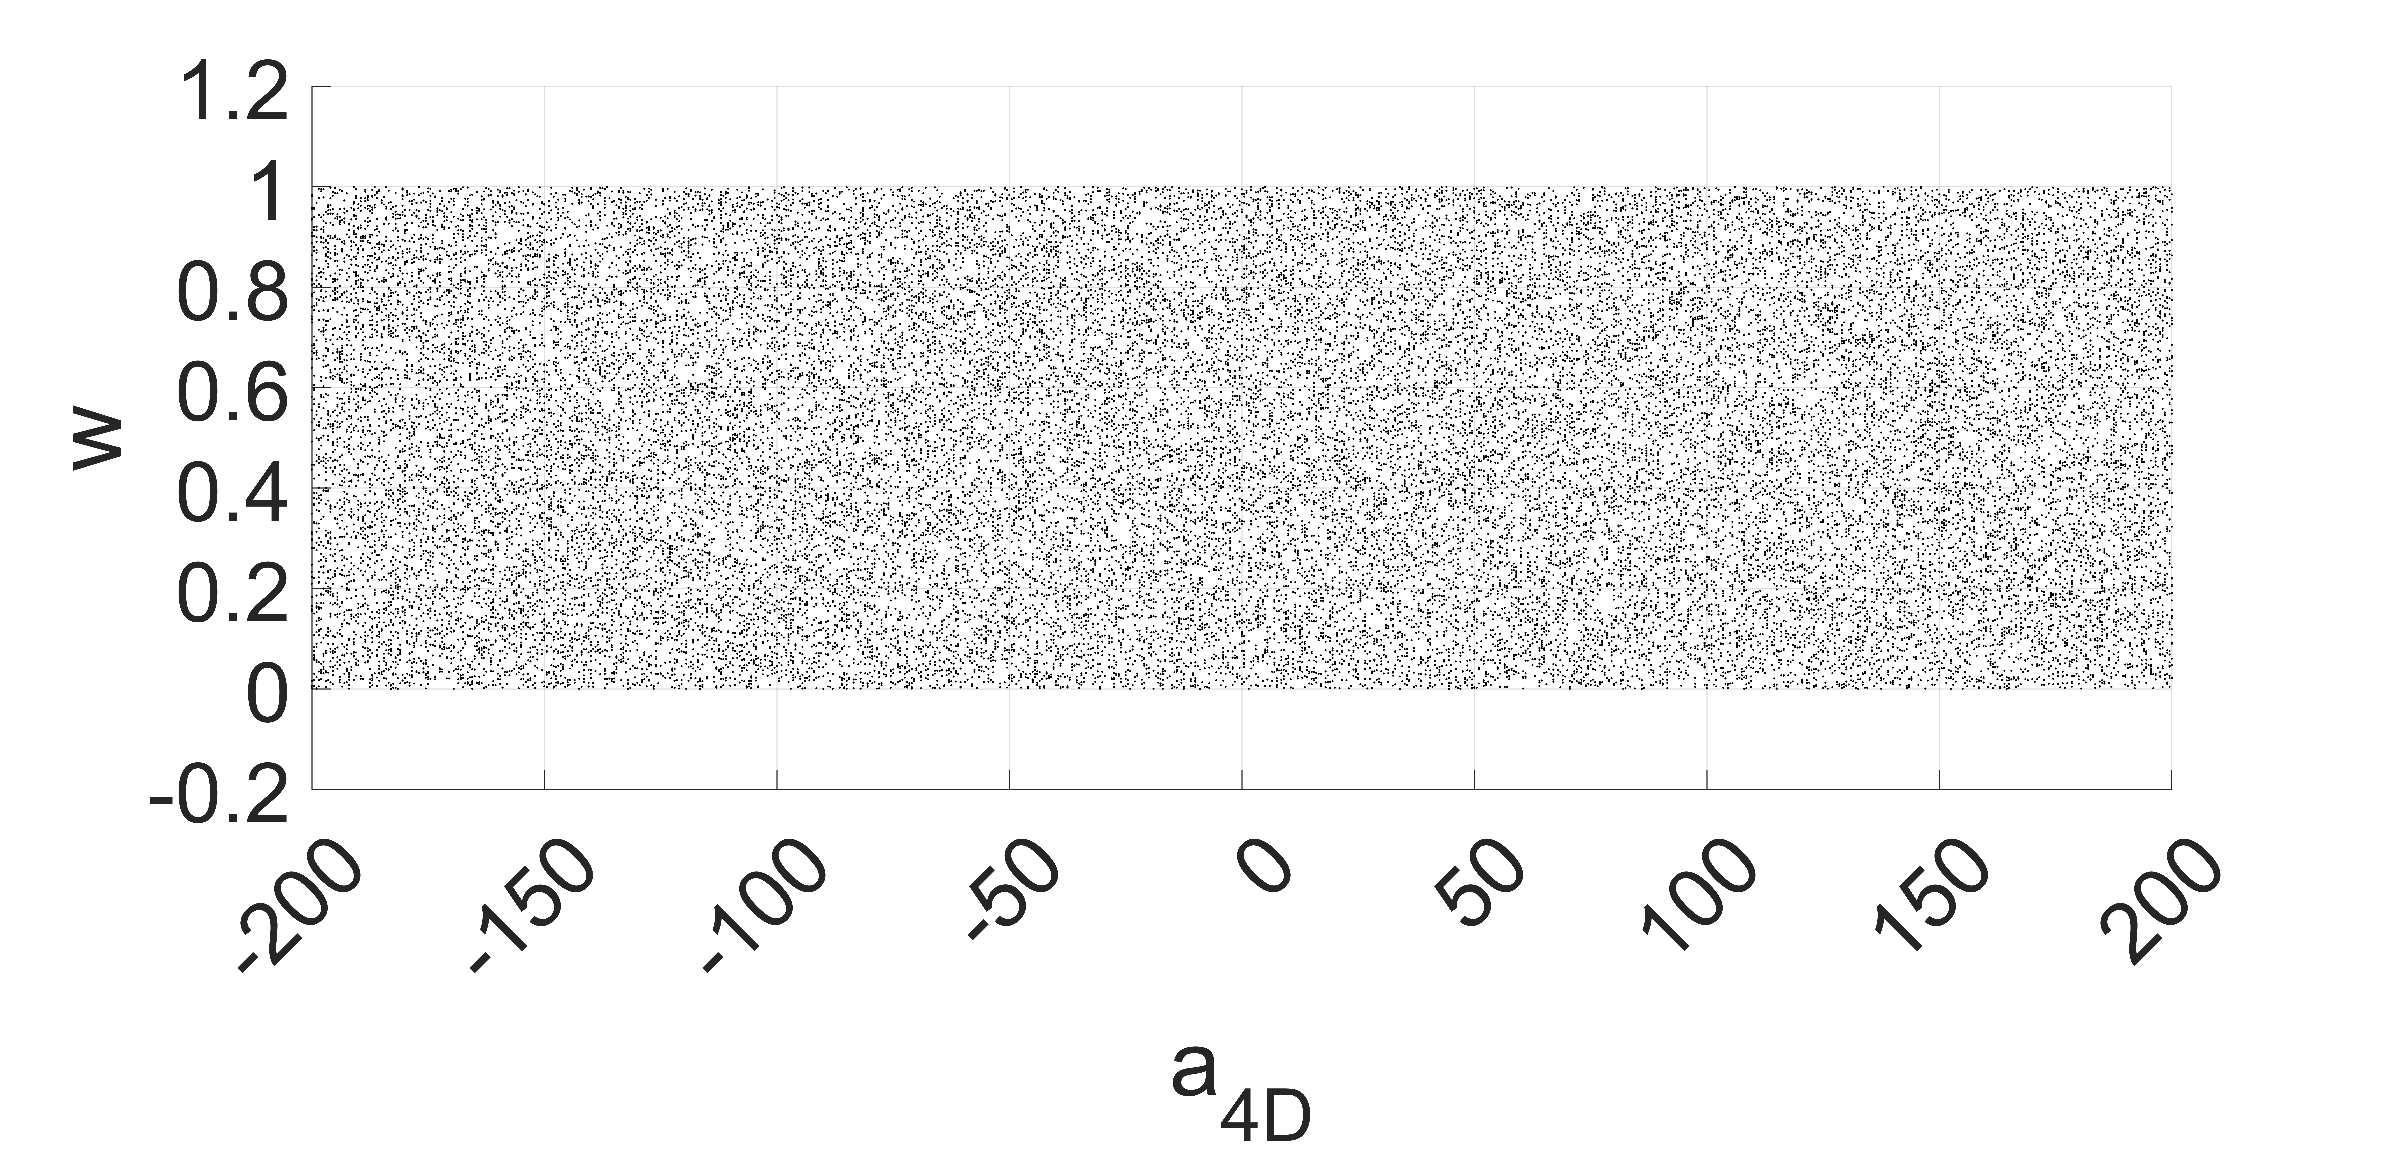
\includegraphics[width=0.48\textwidth]{Figuras IEEE/bifurcation_4D_EHC4S/d.pdf}}% 5

\caption{The 4D-EHC4S bifurcation diagram as a $a_{4D}$ parameter sweep. (a) $x$ state. (b) $y$ state. (c) $z$ state. (d) $w$ state.}
\label{fig_3.5}
\end{figure*}

\subsection{2D Hyperchaotic Map with amplitude control system}
The discrete 2D system 2D-HCAC is described by the map in Eq. \ref{eq_3}, with the states $U_n=(u_n,v_n)^T$ and parameters $ParU = (a_{2D},b_{2D},c_{2D},d_{2D})^T$. The attractor is shown in Figure \ref{fig_4}.
\begin{equation}
\begin{split}
 U_{n+1} &=
\left(\begin{array}{l}
    a_{2D} u_n + b_{2D} u_n |v_n| \\
    c_{2D} u_n + d_{2D} v_n
\end{array}\right)\\
&= {\text{2D-HCAC}}(U_n,ParU)
\end{split}
\label{eq_3}
\end{equation}

\begin{figure}[!t]
\centering
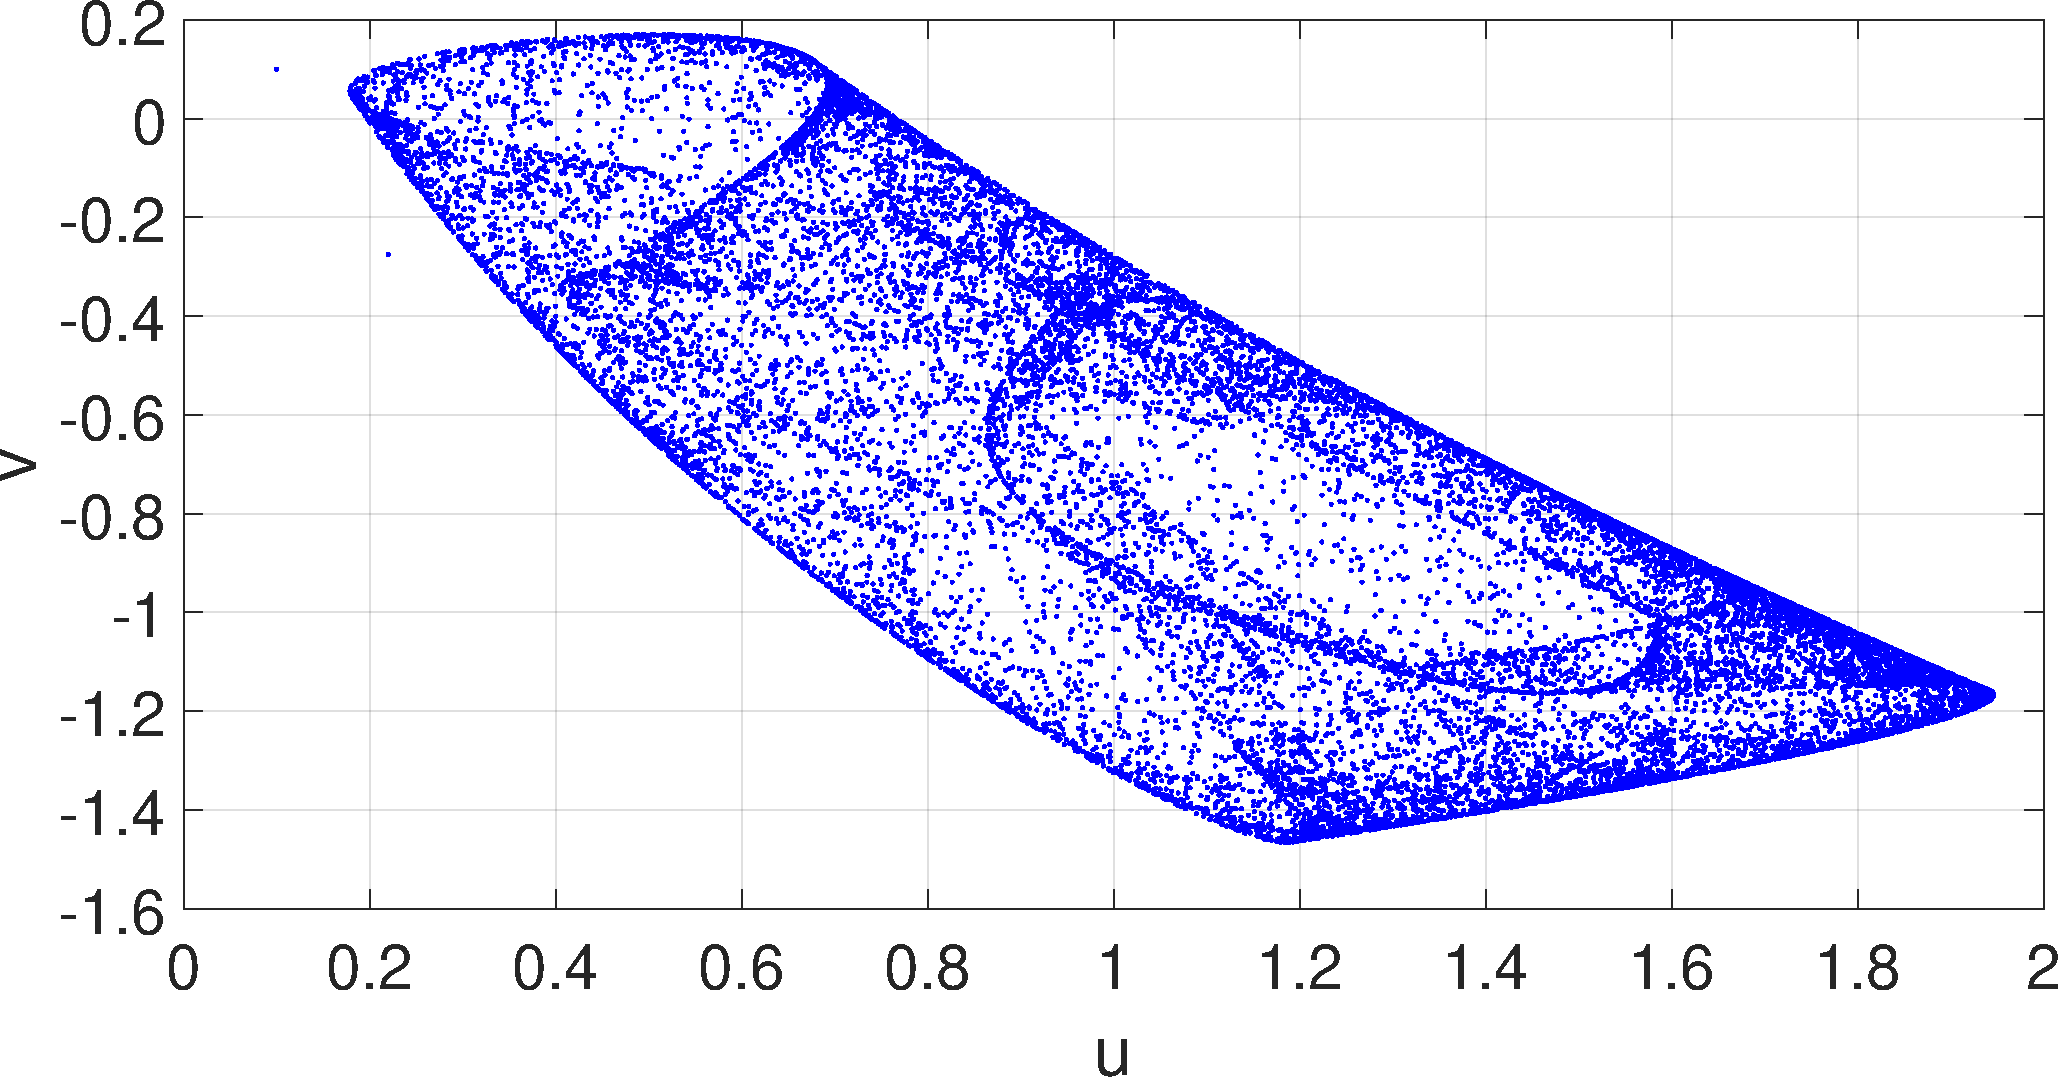
\includegraphics[width=0.73\textwidth]{Figuras IEEE/atractores_2D_HCAC.pdf}
\caption{2D-HCAC phase space diagram.\label{fig_4}}
\end{figure}

The system demonstrates hyperchaotic behavior when the parameters are set to $ParU = (2.35,-1.5,-1.5,-1.25)^T$ and the initial conditions $U_0=(0.1,0.1)^T$. Under these conditions, the system produces two positive LEs, $LE_1=0.1905$ and $LE_2=0.09531$, which confirms its hyperchaotic nature.

The 2D-HCAC system maintains its hyperchaotic dynamics within the parameter ranges $a_{2D}\in[2.29,2.4]$, $b_{2D}\in[-1,-5]$, $c_{2D}\in[-1,-10]$ and $d_{2D}\in[-1.3,-1.12]$. 

The bifurcation diagram presented in Figure \ref{fig_5}, further corroborates this behavior, aligning closely with the observations of the Lyapunov exponents.
\begin{figure*}[!t]
\centering
\begin{subfigure}{0.48\textwidth}
    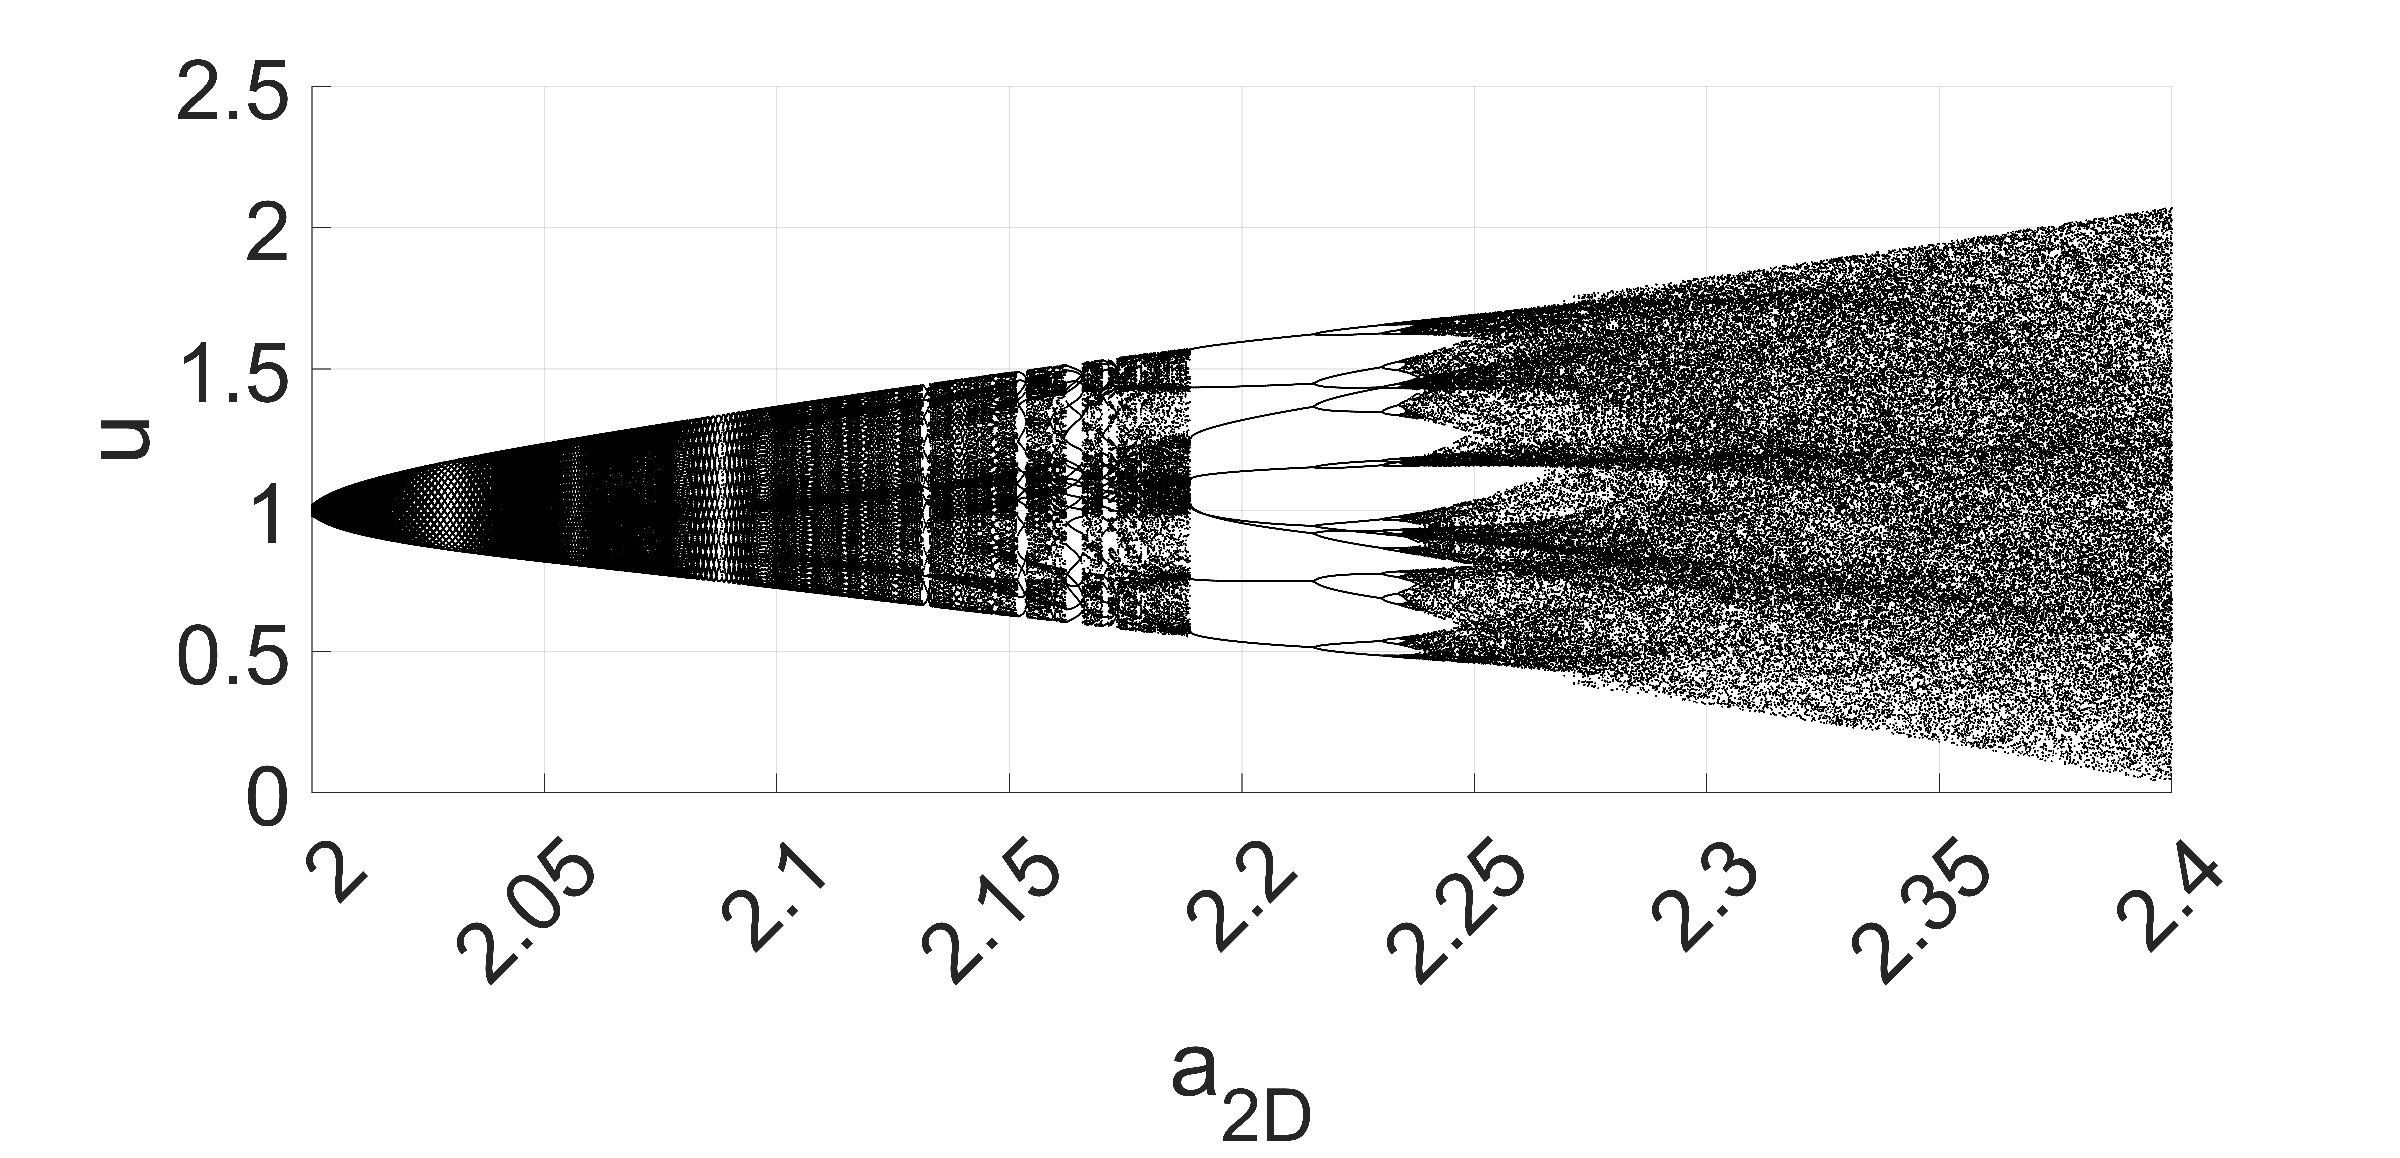
\includegraphics[width=\linewidth]{Figuras IEEE/bifurcation_2D_HCAC/a.pdf}
    \caption{}
\end{subfigure}
\hfill
\begin{subfigure}{0.48\textwidth}
    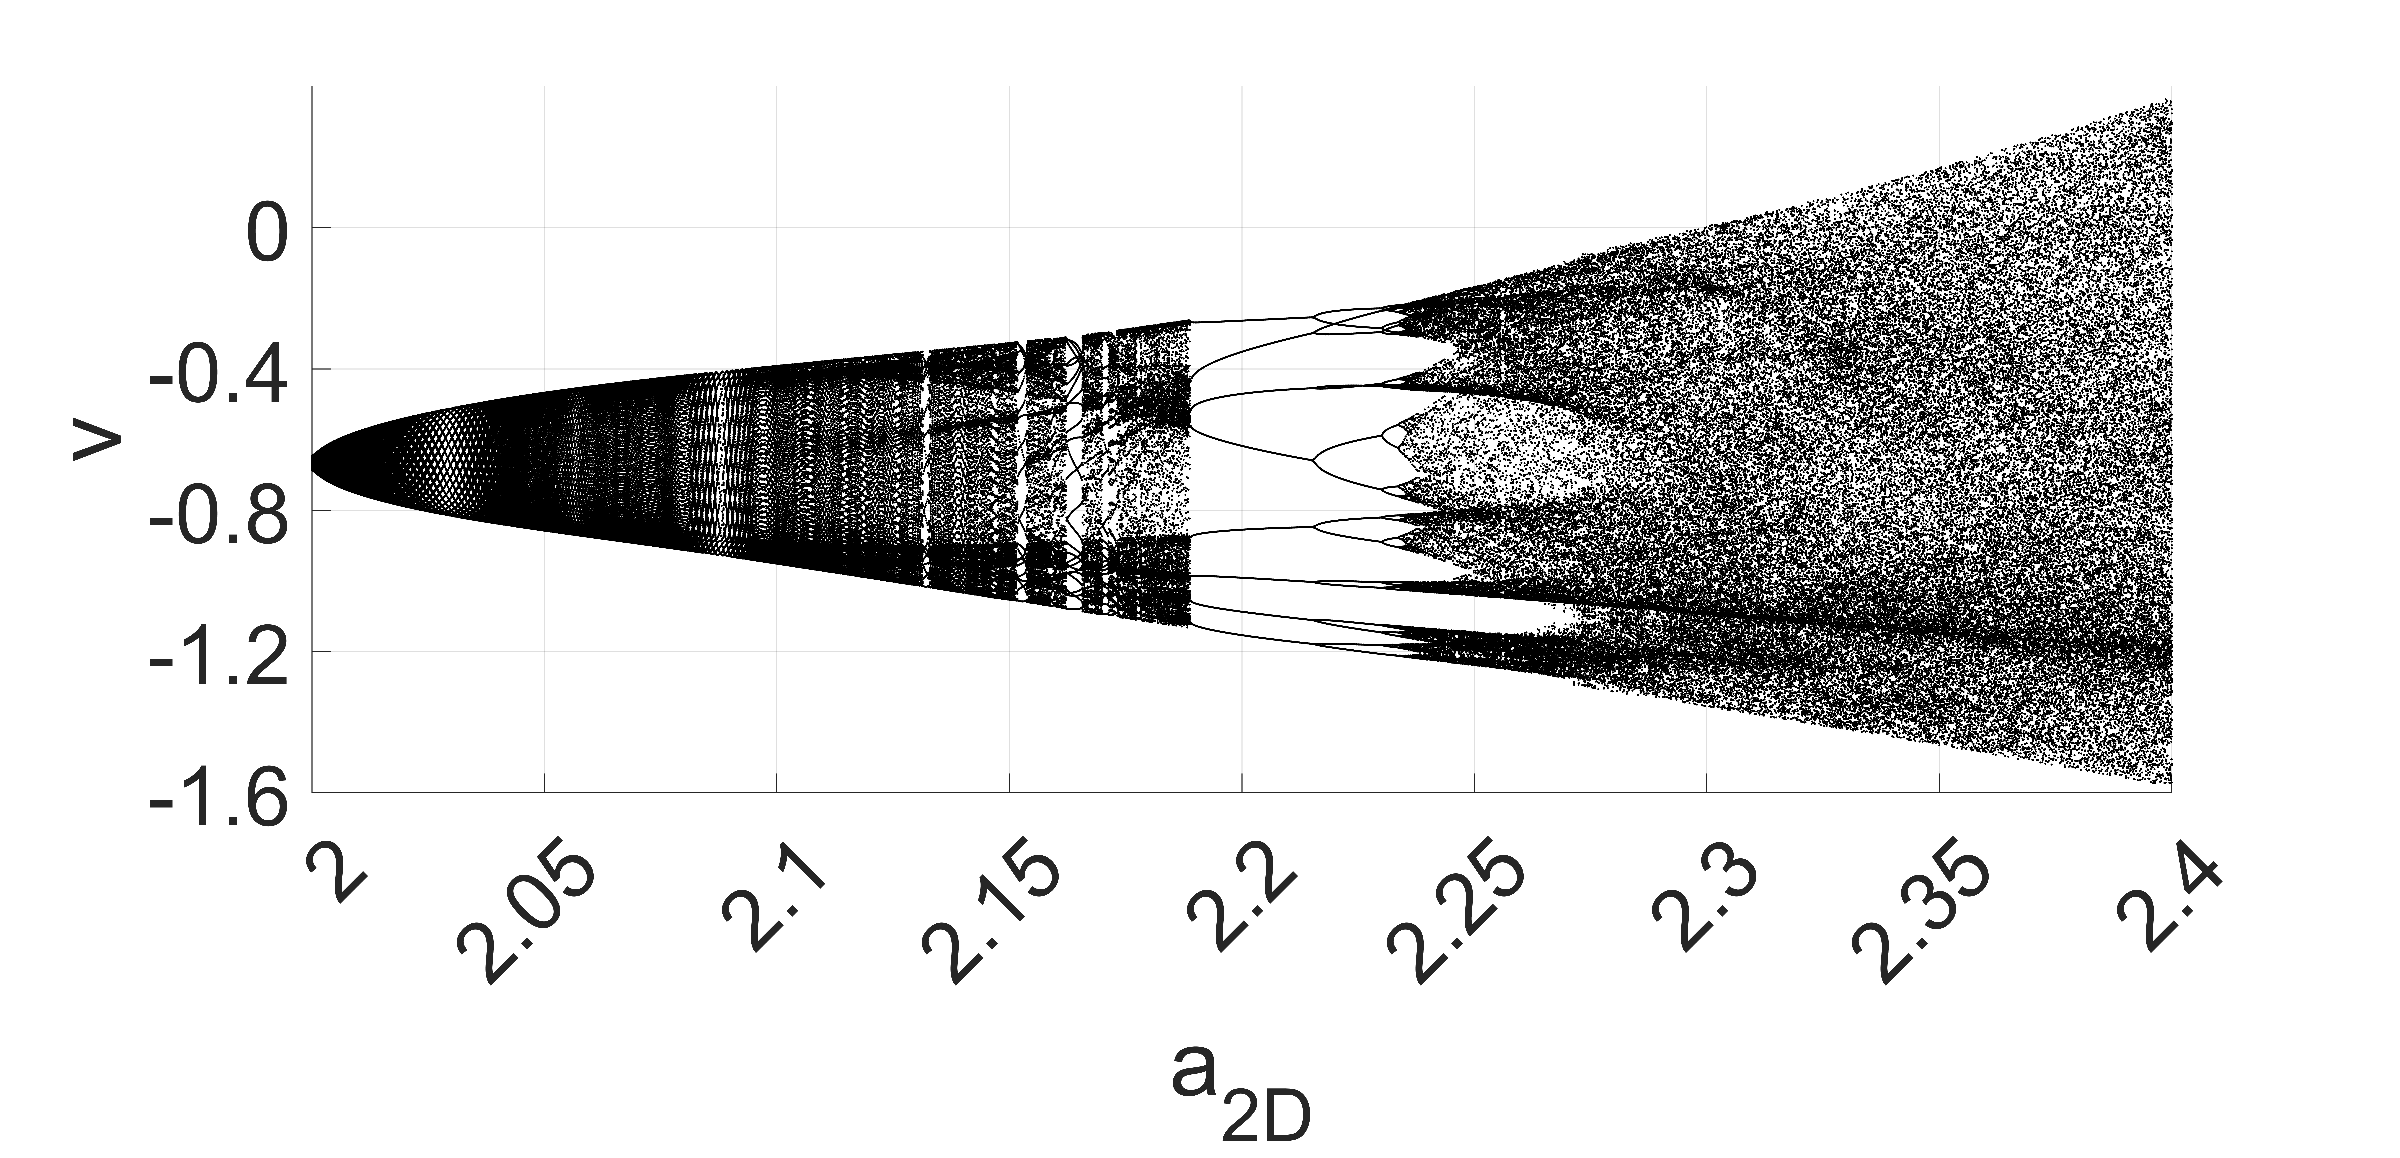
\includegraphics[width=\linewidth]{Figuras IEEE/bifurcation_2D_HCAC/b.pdf}
    \caption{}
\end{subfigure}

\caption{The 2D-HCAC bifurcation diagram as a $a_{2D}$ sweep. (a) $u$ state. (b) $v$ state.}
\label{fig_5}
\end{figure*}

{\color{red}
\subsection{Paramaters and perturbations selection}
To optimize resource usage, all states and parameters are represented using signed fixed-point arithmetic. Custom Q formats were assigned to each variable based on its dynamic range and the precision required to preserve the system's chaotic behavior. In particular, the parameters and states of both systems must be maintained at a precision such that marginal quantization errors do not affect their chaotic dynamics. The system parameters were selected to strictly match those specified in the original publications. Deviating significantly from these nominal values can cause the system to exit the chaotic regime, converge to periodic orbits, or exhibit instability.

A perturbation margin of $\Delta_m=\pm2^{-5}$ was determined to be the safe threshold for the 2D-HCAC system. Since two distinct perturbation sources must be accounted for, parametric perturbation and key integration, the latter requiring 16 bits of precision, a standard fractional precision of $\Delta_{st}=\pm2^{-21}$ was adopted for most variables. The same fractional presicion was used for the states of 4D-EHC4S, though their overall precision shouldn't greatly affect the system's behavior, due to the presence of the multiplier.

In the 4D-EHC4S system, the modular multiplication module effectively dictates the largest Lyapunov exponents (LEs). Because of this dominance, the system reliably achieves hyperchaotic dynamics over a wide parameter space, reducing the sensitivity of the design to exact parameter selection. Nevertheless, the system's behavior is constrained at extreme parameter limits. Although the phase space remains bounded, excessively high parameter values cause the differential derivatives to grow by orders of magnitude. This results in highly stiff differential equations, which require drastically reduced numerical integration step sizes and consequently demand substantially higher computational power.

Regarding the parameter for modular multiplication, a sweep of values was made for multiple sets of lengths, the chi-square p-value was measured looking to optimize this value for the multiple output lengths. 12227 has been choosen empirically in order to maximize the uniformity of the system output. This variable needs to be big enough to effectively mix the various parts of the dimension, while not to big to cause high computational overhead.
The results can be seen in figure \ref{fig_multi}.
\begin{figure}[!ht]
\centering
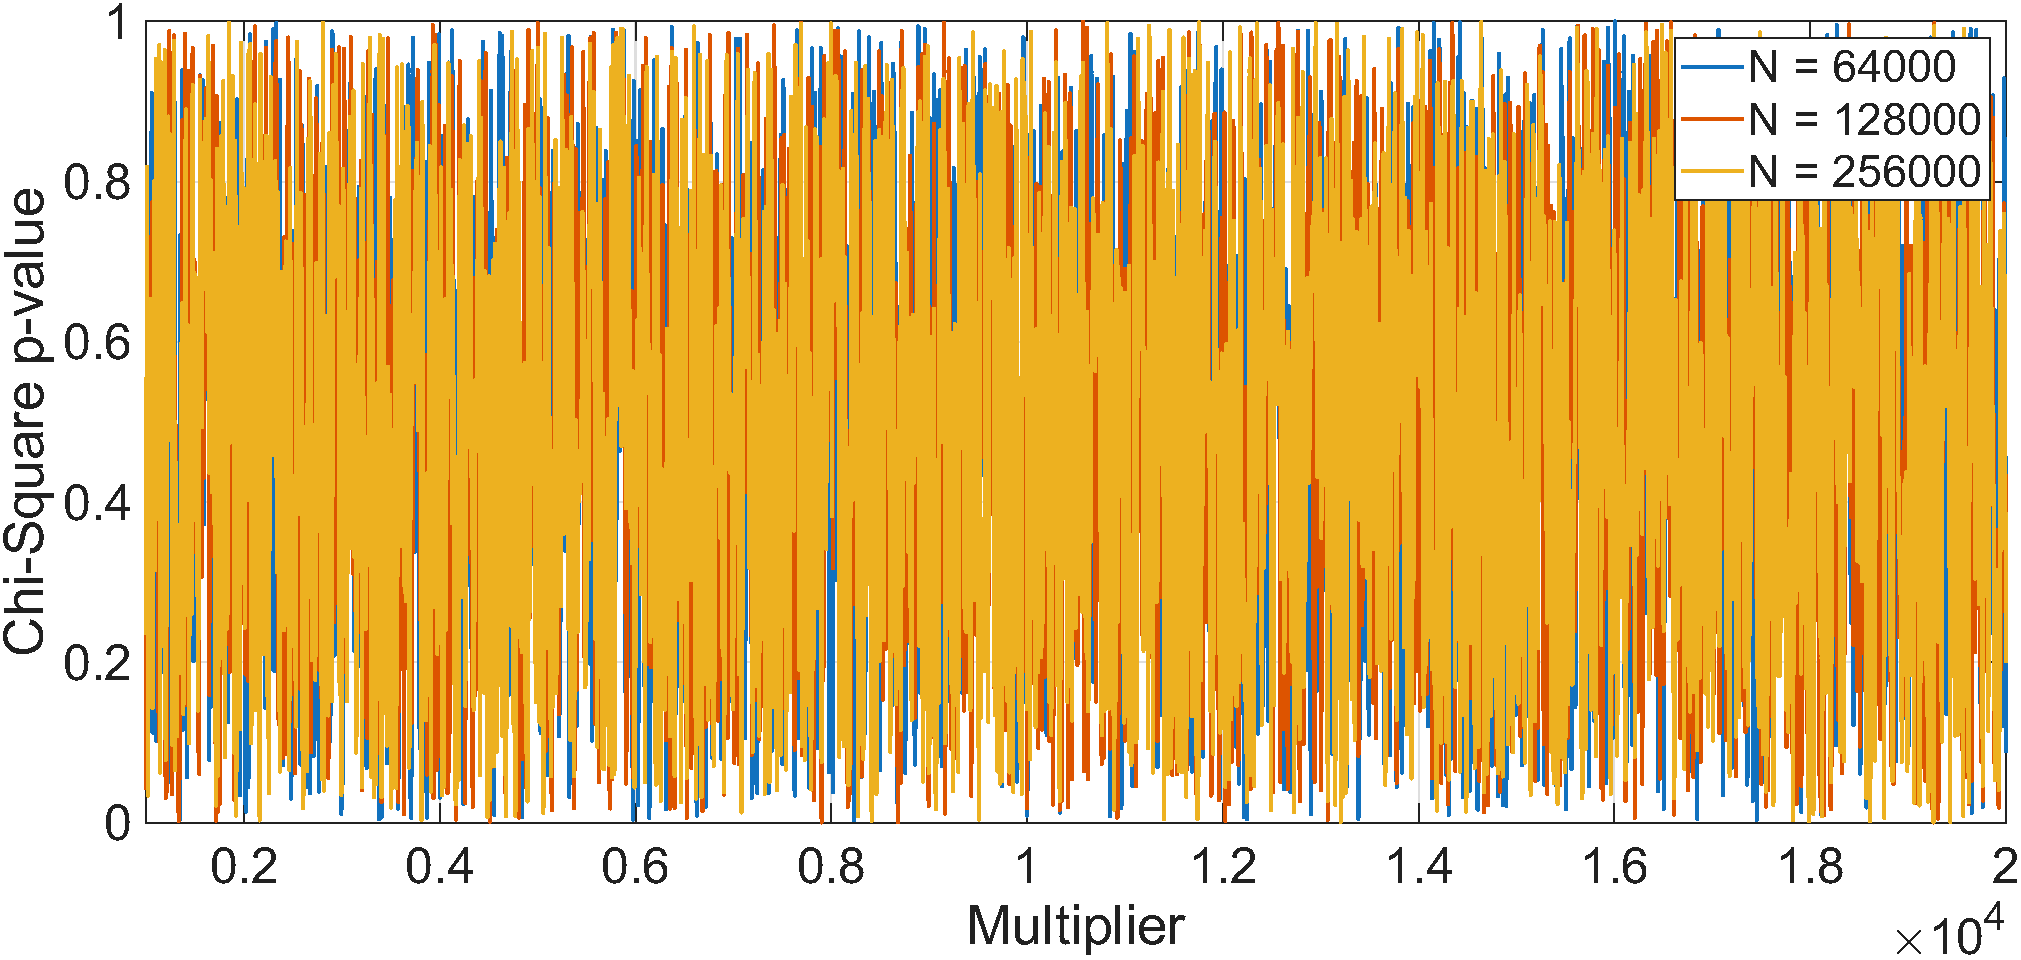
\includegraphics[width=0.72\textwidth]{Figuras IEEE/Multi_histo_chi.pdf}
\caption{Multiplicator sweep.\label{fig_multi}}
\end{figure}



The format of the variables for each system and their precision can be seen in Table \ref{tab_1}.
}

\begin{table}[h]
\centering
\footnotesize
\begin{tblr}{
  colspec = {c c c c},
  row{1} = {font=\bfseries},
  hline{1,2,Z} = {solid}, 
}
Variable & Format (Qn.m) & Variable limits & Precision \\
$ParX$ & Q6.21 & $[-32, 32)$ & $2^{-21}$ \\
$XE$ & Q1.31 & $[-1, 1)$ & $2^{-21}$ \\
$ParU$ & Q3.21 & $[-4, 4)$ & $2^{-21}$ \\
$U$ & Q3.21 & $[-4, 4)$ & $2^{-21}$ \\
$h$ & Q1.21 & $[-1, 1)$ & $2^{-21}$ \\
\end{tblr}
\caption{Systems variable formats.}\label{tab_1}
\end{table}

\subsection{Parametric perturbations}
To limit the problem of short cycles within the system, parametric perturbations are applied. This involves making small controlled changes to the parameters or states of a system during each iteration, thereby preventing the system from repeating its past behavior \cite{hocine_prng_2023, liu_hardware_2020}. As mentioned above, the complementary module (2D-HCAC) of the PRNG will be used to introduce these perturbations into the primary module (4D-EHC4S). 

Sixteen bits are extracted from the two states of the complementary module and divided into four 8-bit sequences, which are distributed among the four parameters of the primary module. In the following equations, the notation var[a : b] denotes the extraction of the binary sequence from bit position 'a' to bit position 'b' of the fractional part of the variable. The perturbations are carefully scaled to affect the least significant bits of each variable. The system is then perturbed by adding these values to the respective parameters, as shown in Eq. \ref{eq_6} and Eq. \ref{eq_7}.
\begin{align}
\label{eq_6}
Pert(U_n) &=
\left(\begin{array}{l}
    u_n\left[-14:-21 \right]\\
    u_n\left[-6:-13 \right] \\
    v_n\left[-14:-21 \right] \\
    v_n\left[-6:-13 \right] \\
\end{array}\right)\\
\label{eq_7}
ParX_{n+1}&= ParX_0+2^{-13}Pert(U_n)
\end{align}

\subsection{Post-Processing}

A post-processing module is incorporated in the final stage of the PRNG to introduce additional nonlinearities into the generated output, enhancing its cryptographic strength. A common and effective technique for this purpose is the use of a simple XOR gate \cite{benkouider_novel_2024, dridi_design_2023, dridi_design_2022}, which combines multiple state outputs. First, the 8 least significant bits (LSB) are extracted from each of the four primary states, Eq. \ref{eq_8}.
\begin{equation}
Xb_{n} = XE_n\left[-14:-21 \right]
\label{eq_8}
\end{equation}

A multiplexer then dynamically selects three of these four LSB streams, $SIG_n = (SIG_{n,0}, SIG_{n,1}, SIG_{n,2})^T$, with the selection signal, $SEL_n$, derived from two bits of the complementary system state, Eq. \ref{eq_9} and \ref{eq_10}.
\begin{align}
\label{eq_9}
SEL_n &= u_n\left[-20:-21 \right] \in \left\{0,1,2,3\right\} \\
\label{eq_10}
\begin{split}
SIG_n &=
  \left(\begin{array}{l}
    Xb_{n, (SEL_n \bmod 4}) \\
    Xb_{n, ((SEL_n+1) \bmod 4}) \\
    Xb_{n, ((SEL_n+2) \bmod 4})  
  \end{array}\right)\\
&=Mux(Xb_n,SEL_n)
\end{split}
\end{align}

Finally, these three selected streams are combined via an XOR operation to produce the 8-bit PRNG output expressed in Eq. \ref{eq_11}.
\begin{equation}
\begin{aligned}
    PRNG_n &= SIG_{n,0} \oplus SIG_{n,1} \oplus SIG_{n,2} \\
\end{aligned}
\label{eq_11}
\end{equation}

\section{Hardware implementation}\label{sec_4}
\subsection{Hardware}
For the hardware realization of this work, the Terasic DE2-115 development board serves as the platform for this work. This robust development board is equipped with an Altera Cyclone IV E EP4CE115F29C7 FPGA chip with a {\color{red} clock frequency of 50 MHz clock}. This FPGA is a commonly adopted choice in contemporary research efforts  \cite{meranza-castillon_pseudorandom_2019} due to its advantageous balance of cost-effectiveness, low power consumption, and substantial logic resources.

Using an 8-bit output width for the PRNG yields a throughput of 400 Mb/s. While increasing the output width could achieve higher throughput, it may also degrade the quality of the generated random sequence.

To enable efficient transmission of the generated data for analysis, the simple UART protocol (Universal Asynchronous Receiver/Transmitter) will be used.

\subsection{Key integration}
To initiate pseudorandom sequence generation, a key is used to alter the system variables. By modifying the initial conditions and parameters of both the primary and complementary chaotic modules, this key ensures that the PRNG produces a unique sequence for every different key.

The system utilizes a 224-bit key, and this key is divided into 16-bit segments. These segments are scaled to a predefined margin of $\Delta_k=\pm2^{-6}$ for the chaotic systems used to retain their hyperchaotic properties within their respective operational ranges. The segments are then allocated to each of the 14 variables across both chaotic modules. The initialization of the system states and parameters is defined by $var_b$ as the base value and $var_0$ as the initial value at the first iteration, which is expressed in Eq. \ref{eq_12} and Eq. \ref{eq_13}. Table \ref{tab_2} provides a detailed key bit distribution.
\begin{align}
\label{eq_12}
K_i &= KEY\left[223-16i:208-16i\right] \\
\label{eq_13}
var_{0,i} &= var_{b,i}+2^{-21}K_i
\end{align}

\begin{table}[h]
\centering
\footnotesize
\begin{tblr}{
  colspec = {ccc},
  row{1} = {font=\bfseries},
  hline{1,2,Z} = {solid},
}
Variable ($var$) & Variable base value ($var_b$) & Key bits ($KEY$) \\
$ParX$ & $(9, 27, 8, 0.1)^T$ & $(K_0, K_1,$ $K_2, K_3)^T$ \\
$XE$ & $(0.3, 0.2, 0.2, 0.3)^T$ & $(K_4, K_5,$ $K_6, K_7)^T$ \\
$ParU$ & $(2.35, -1.5,$ $-1.5, -1.25)^T$ & $(K_8, K_9,$ $K_{10}, K_{11})^T$ \\
$U$ & $(0.1, 0.1)^T$ & $(K_{12}, K_{13})^T$ \\
\end{tblr}
\caption{Key bit allocation to system variables}
\label{tab_2}
\end{table}
\subsection{PRNG architecture}
The overall architecture and interconnections of the various modules within the PRNG are schematically represented in Figure \ref{fig_9}. This diagram illustrates how the complementary module (mod comp) generates perturbations on the parameters of the primary module (mod prim). The primary and complementary modules then transmit their respective data to the post-processing module (mod postp), which is responsible for synthesizing the final output of the PRNG.
{\color{red}
To ensure the necessary buffer capacity for the system, the primary module was subdivided into six processing stages. This architectural choice was implemented to enhance pipeline efficiency and prevent data bottlenecks.}
The entire sequence generation process is shown by the steps outlined in Algorithm \ref{alg_1}.
\begin{figure} [!ht]
\centering
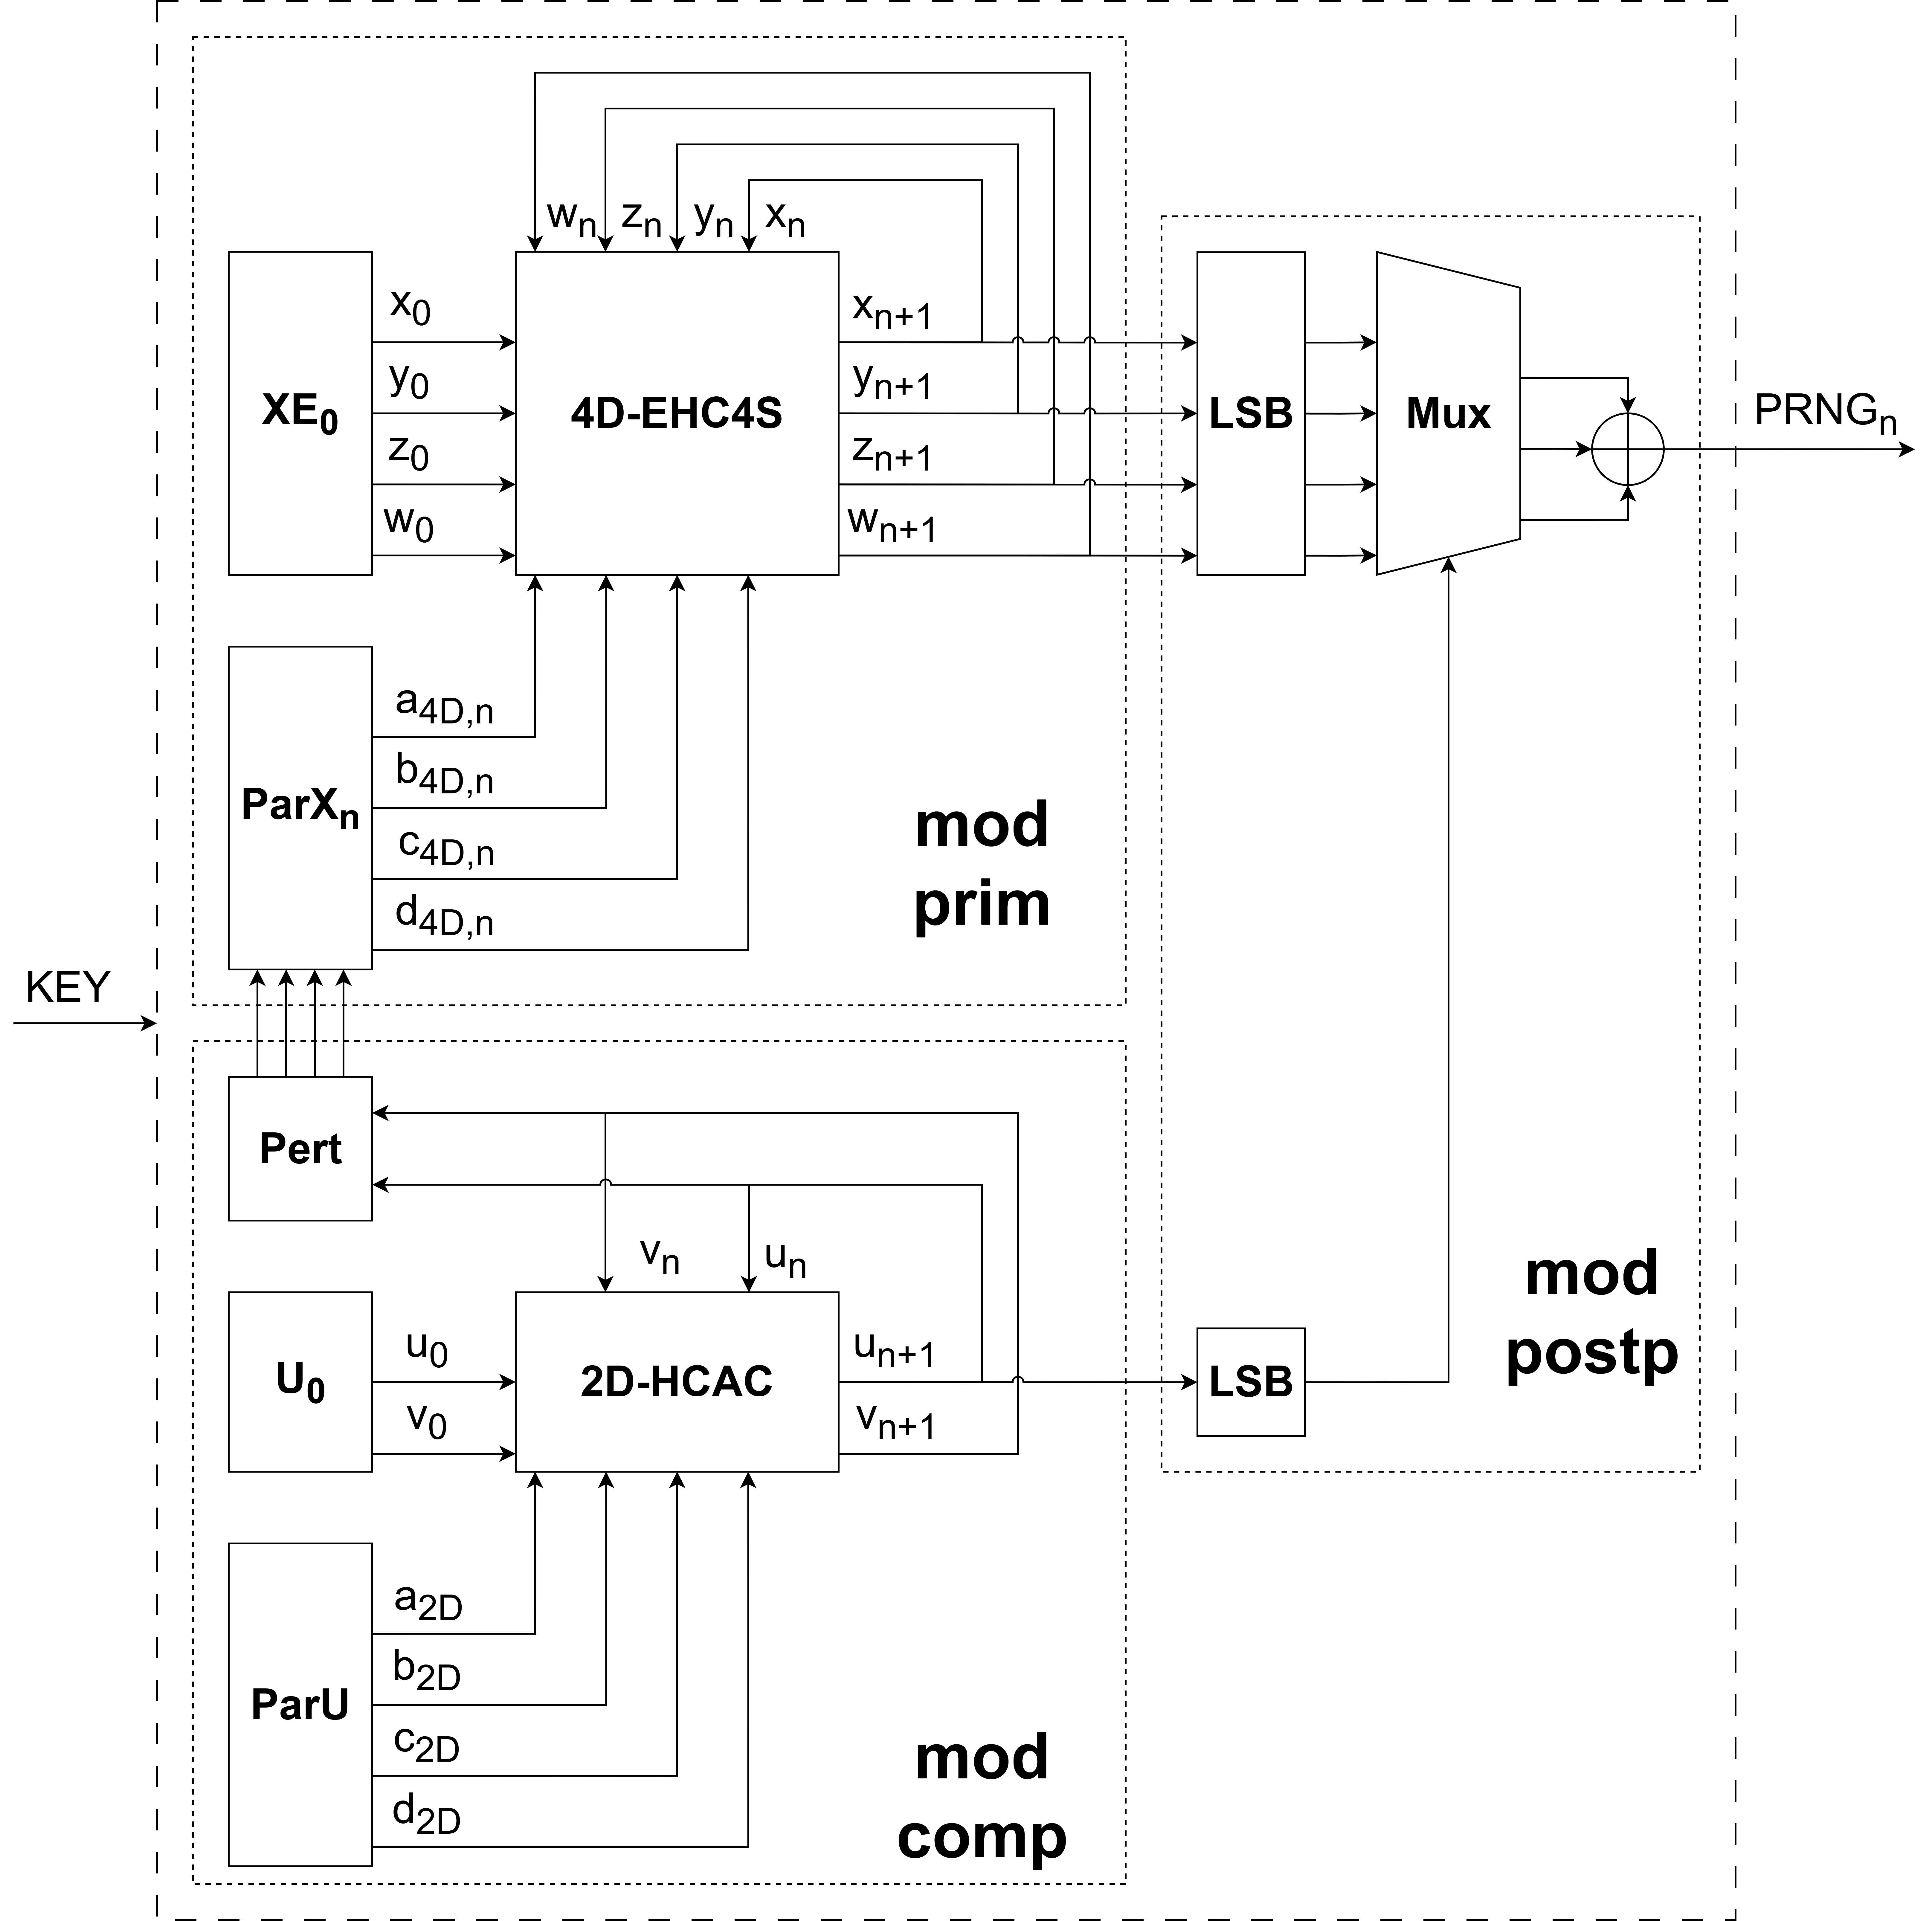
\includegraphics[width=0.8\textwidth]{Figuras IEEE/Diagrama PRNG Articulo(3).png}
\caption{Schematic of the proposed PRNG.\label{fig_9}}
\end{figure}

\begin{algorithm}[!ht]
\caption{\enskip PRNGs pseudocode.}\label{alg_1}
\begin{algorithmic}[1]
  \State $KEY$
  \Comment{Input}
  \State $K_0 \ldots K_{13} \gets \text{split} (KEY,16)$
  \State $ParX_b \gets (9, 27, 8, 0.1)^T$
  \Comment{4D-EHC4S parameters and ICs}
  \State $ParX_0 \gets ParX_b + 2^{-21}(K_0, K_1, K_2,K_3)^T $
  \State $XE_b \gets (0.3, 0.2, 0.2, 0.3)^T$
  \State $XE_0 \gets  XE_b + 2^{-21}(K_4, K_5, K_6,K_7)^T$
  \State $ParU_b \gets (2.35, -1.5, -1.5, -1.25)^T$
  \Comment{2D-HCAC parameters and ICs}
  \State $ParU \gets  ParU_b + 2^{-21}(K_8, K_9, K_{10},K_{11})^T $
  \State $U_b \gets (0.1,0.1)^T$
  \State $U_0 \gets  U_b + 2^{-21}(K_{12},K_{13})^T$
  \For{$n=0$ to $N$}
    \Comment{System iterations}
    \State $U_{n+1} \gets \text{2D-HCAC}(U_{n}, ParU)$
    \State $XE_{n+1} \gets \text{4D-EHC4S}(XE_n, ParX_n)$
    \State $ParX_{n+1} \gets  ParX_{0} + 2^{-13}Pert(U_n)$
    \Comment{Parametric perturbation}
    \State $Xb_n \gets XE_{n}[-14:-21]$
    \Comment{Selector}
    \State $SEL_n \gets u\left[-20:-21\right]$
    \State $SIG_{n,0} \gets Xb_{n,SEL \% 4}$
    \State $SIG_{n,1} \gets Xb_{n,((SEL+1) \% 4)}$
    \State $SIG_{n,2} \gets Xb_{n,((SEL+2) \% 4)}$
    \State $PRNG_n  \gets SIG_{n,0} \oplus SIG_{n,1} \oplus SIG_{n,2}$
    \Comment{Output}
  \EndFor
\end{algorithmic}
\end{algorithm}

As mentioned before, the proposed PRNG is initialized with a 224-bit key to generate a pseudorandom sequence of integers in the range $[0,255]$. Each key determines a unique output sequence. Using the keys listed in Table \ref{tab_3.5}, the corresponding generator outputs are shown in Figure \ref{fig_9.5}.
\begin{table}[!ht]
\centering
\begin{tblr}{
  colspec = {cc},
  row{1} = {font=\bfseries},
  hline{1,2,Z} = {solid}, % Top, after header, and bottom
}
Key & Value \\
KEY A & {$0000000000000000\_0000000000000000\_$ \\ $0000000000000000\_00000000_{16}$} \\
KEY B & {$3C8D9A2B7F0E1654\_A9D8C7B6F5E43210\_$ \\ $B9A8D7C6F5E43210\_B9A8D7C6_{16}$} \\
KEY C & {$AABBCCDDEEFF0011\_2233445566778899\_$ \\ $AABBCCDDEEFF0011\_22334455_{16}$} \\
\end{tblr}
\caption{Keys for PRNG trajectory visualization.}
\label{tab_3.5}
\end{table}

\begin{figure}[!ht]
\centering
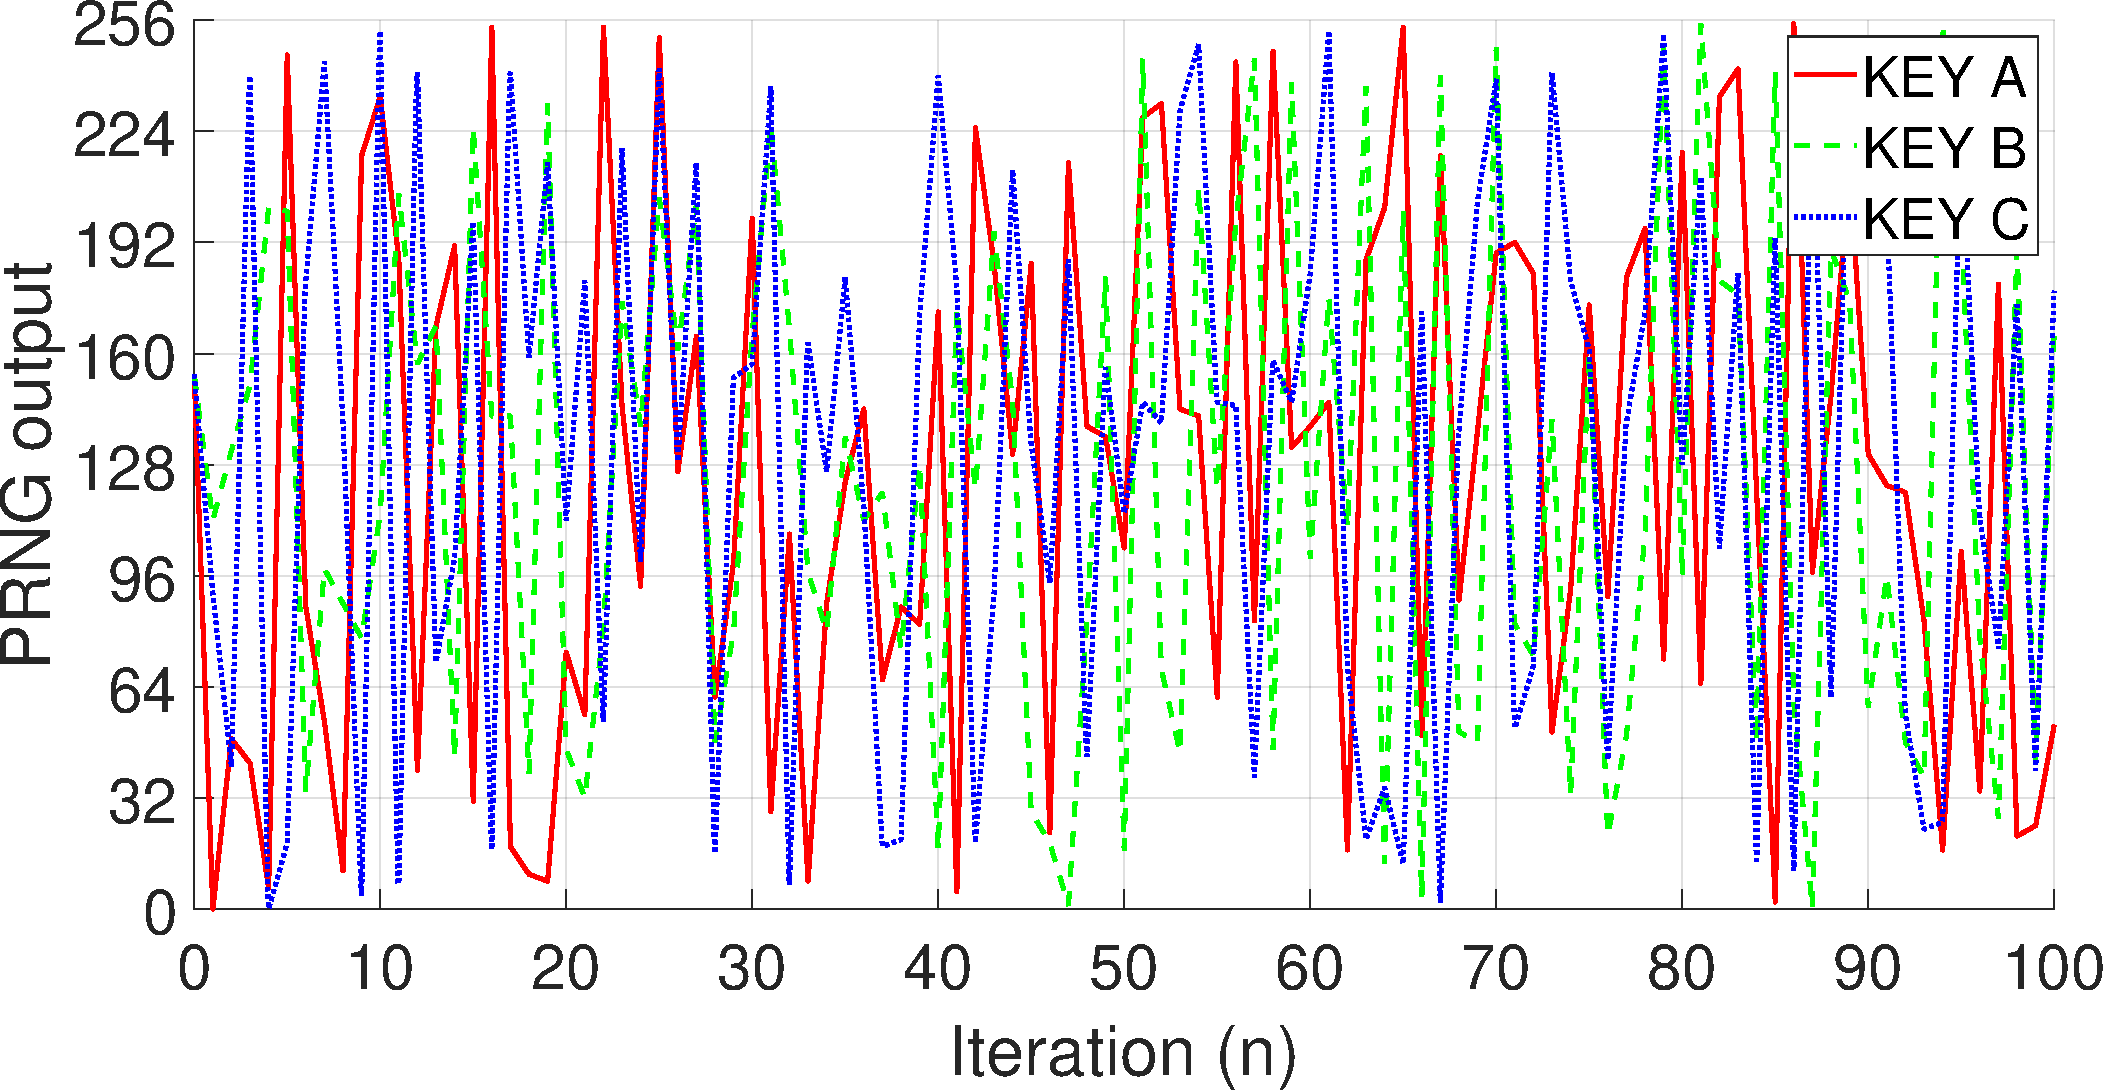
\includegraphics[width=0.72\textwidth]{Figuras IEEE/PRNG_MAT_Results.pdf}
\caption{PRNG trajectory, using different keys.\label{fig_9.5}}
\end{figure}

\section{Eficiency and security analysis}\label{sec_5}
This section shows the results of several chaos and randomness tests to ensure suitability for cryptographic use. 
\subsection{Resources used}
An analysis of the computational resources consumed by the PRNG confirms that the PRNG implemented is not resource intensive and will not limit other functionalities within the platform. Table \ref{tab_3} presents a comprehensive overview of the resources used by the PRNG. The PRNG exhibits minimal resource consumption, with most categories utilizing less than $3\%$ of the available resources. In particular, multipliers account for the highest proportion of usage, at $23\%$, showing their role in the arithmetic operations of the system. In this configuration, the system was able to achieve a throughput of 66.6 Mb/s using the FPGA's 50 MHz clock.

\begin{table}[h]
\centering
\footnotesize
\begin{tblr}{
  colspec = {cccc},
  row{1} = {font=\bfseries},
  hline{1,2,Z} = {solid}, % Top, after header, bottom
}
Resource & Amount & Available & Use \\
Total logic elements & $3,646$ & $114,480$ & $3\%$ \\
Total registers & $1,123$ & $117,053$ & $<1\%$ \\
Total pins & $4$ & $529$ & $<1\%$ \\
Total virtual pins & $0$ & -- & -- \\
Total memory bits & $28,672$ & $3,981,312$ & $<1\%$ \\
Embedded Multiplier 9-bit elements & $124$ & $532$ & $23\%$ \\
Total PLLs & $0$ & $4$ & $0\%$ \\
\end{tblr}
\caption{PRNG resource use on FPGA.}
\label{tab_3}
\end{table}

\subsection{Key space}
To effectively resist brute force attacks, a PRNG's key space must be sufficiently large. The proposed PRNG uses a 224-bit key, providing a key space of $2^{224}$ possible keys. This exceeds the NIST recommended minimum key space of $2^{128}$ \cite{barker_transitioning_2019}, providing a robust defense against brute-force cryptanalysis.

{
  \color{red} 
  \subsection{Time analysis}
  ....
}
\subsection{Key sensitivity}
A fundamental characteristic of a cryptographically secure PRNG is its extreme sensitivity to changes in its input key. Even the slightest alteration in the key must result in drastically different output sequences. This property demonstrates a high degree of unpredictability in the PRNG's output and proves resistance to exploitation of underlying patterns.

To evaluate this property, the normalized Hamming distance was measured between two output sequences generated from keys differing by a single bit. For an ideal PRNG, flipping one bit in the key should result in approximately $50\%$ of the output bits differing, indicating maximal divergence between the two sequences.

{\color{red}
The system was tested using 100 distinct keys, each distinct from a reference key $KEY_\text{ref}$ (see Table \ref{tab_4} for its hexadecimal representation, where underscores serve as visual separators). For each key, 100,000 output bits were generated and compared bitwise to the reference key's output. The normalized Hamming distances resulted in a mean of $49.981\%$ with a normalized standard deviation of $1.499 \times 10^{-3}$,  indicating strong sensitivity to the initial key.
}
\begin{table}[h]
\centering
\begin{tblr}{
  colspec = {cc},
  row{1} = {font=\bfseries},
  hline{1,2,Z} = {solid},
}
Key & Value \\
$KEY_\text{ref}$ & {$0123456789ABCDEF\_0123456789ABCDEF\_$ \\ $0123456789ABCDEF\_01234567_{16}$}
\end{tblr}
\caption{Key reference for Hamming distance.}
\label{tab_4}
\end{table}

\subsection{Uniformity}
A robust PRNG is mandated to produce output sequences that closely approximate a uniform distribution. Any inherent bias or tendencies in the generated values directly compromises the PRNG's security by increasing its vulnerability to cryptanalysis.
{\color{red}
Output uniformity was evaluated using a histogram of 25,600,000 iterations of 8-bit values generated using $KEY_\text{ref}$ and chi-square test. The frequency of each value should ideally be $1 \times 10^{5}$ for a uniform distribution. As depicted in Figure \ref{fig_11}, the observed frequencies align closely with this ideal.
}

\begin{figure}[h]
\centering
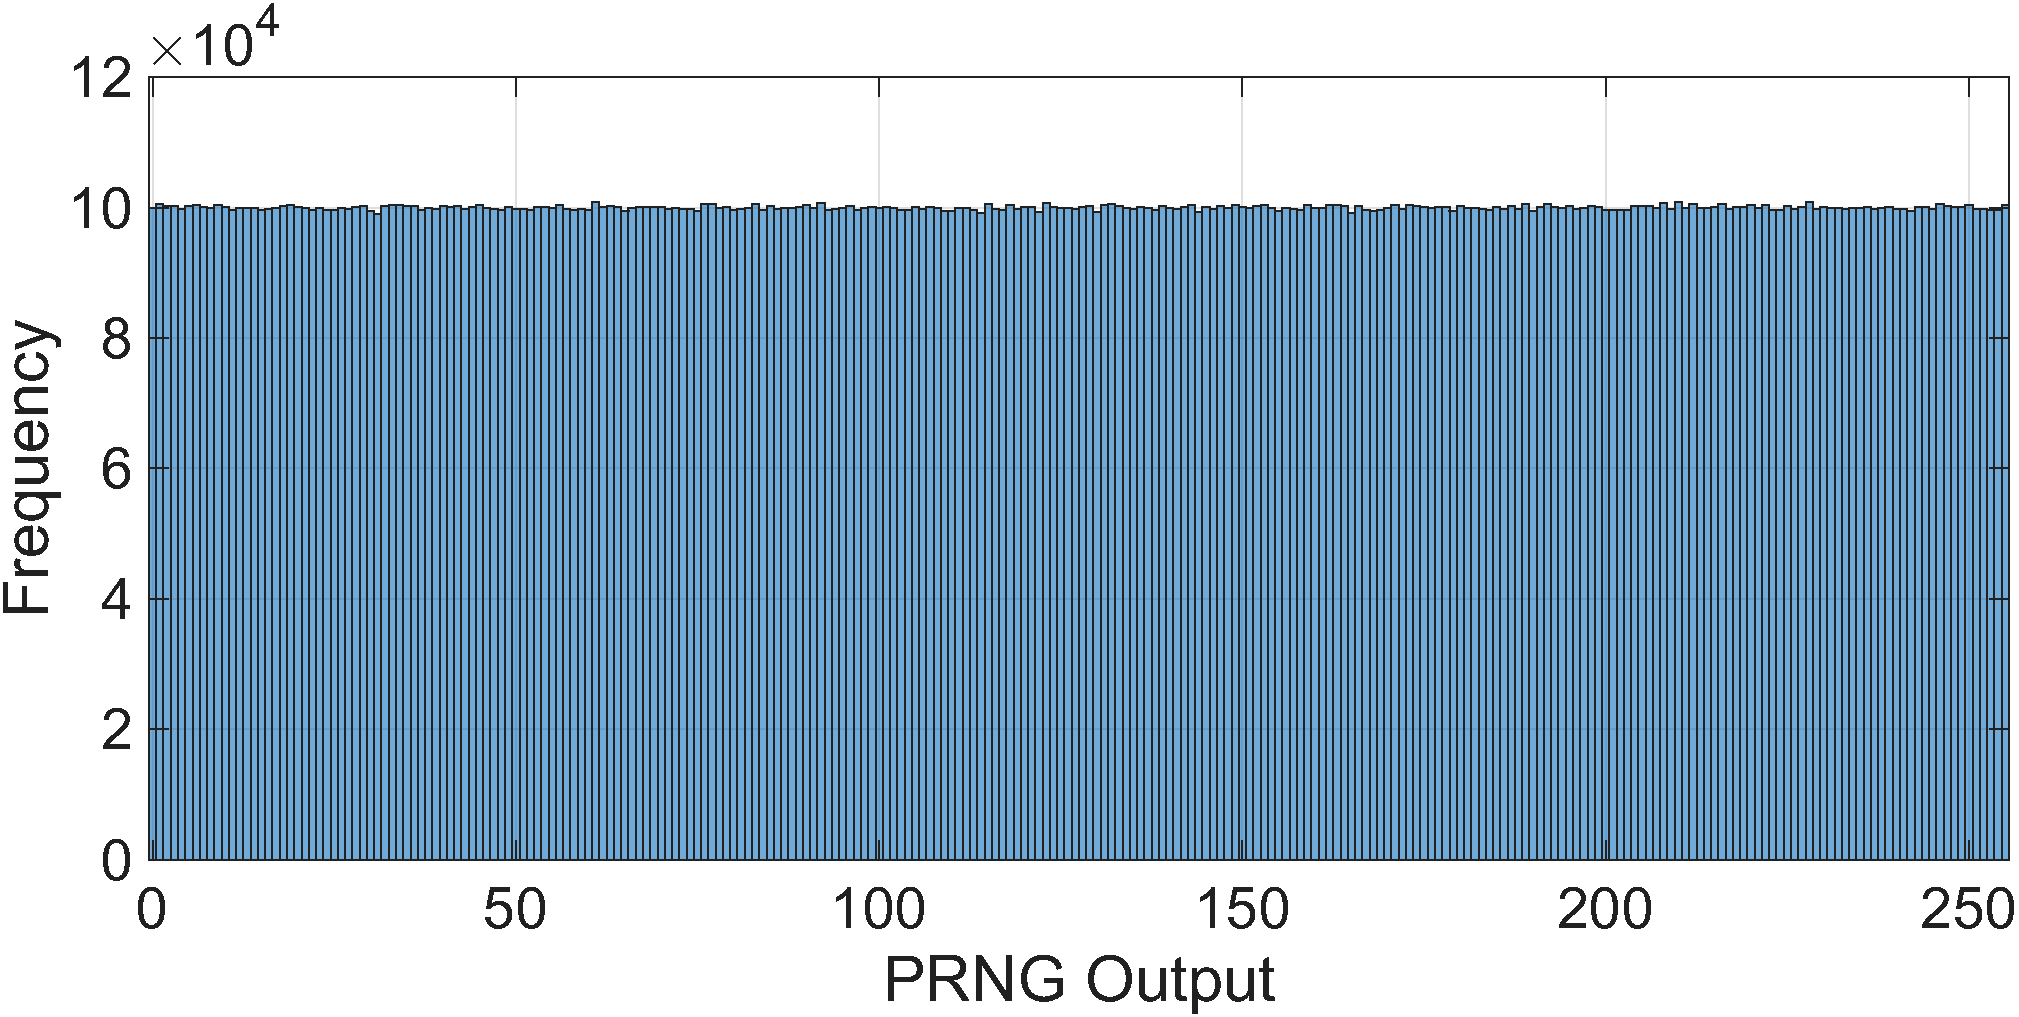
\includegraphics[width=0.72\textwidth]{Figuras IEEE/Histogram_PRNG_FPGA_25_6_MILL.pdf}
\caption{PRNG histogram.\label{fig_11}}
\end{figure}

The resulting chi-square p-value ($p = 0.41631$) exceeded the standard significance level ($\alpha = 0.05$), and the calculated frequency variance, ($S^2 = 1.0162 \times 10^{5}$), closely matches the expected variance of ($S^2 = 0.9961 \times 10^{5}$) for such a uniform distribution. This strongly confirms the uniformity of the PRNG's output.

\subsection{Gottwald-Melbourne 0-1 test for chaos}
Although chaos testing is not typically applied to PRNGs, given that they are not strictly chaotic systems, employing such tests can provide additional support for the notion of chaotic behavior within the PRNG, despite differences in testing methodology.

The 0-1 test, developed by Gottwald-Melbourne \cite{gottwald_new_2004}, assesses chaos by calculating the correlation coefficient $K$ from the time series. A value of $K \approx 1$ indicates chaotic behavior, while $K \approx 0$ indicates a lack of chaos. An analysis of 5,000 sequences generated using $KEY_\text{ref}$ yielded a value $K = 0.9980$, effectively demonstrating chaotic content within the system.

Methods for analyzing the maximum Lyapunov exponent ($LE_{max}$) from a time series prove beneficial in this context. Applying the Rosenstein algorithm \cite{rosenstein_practical_1993} to the PRNG's output resulted in $LE_{max} = 0.674924$. Although this value is smaller than that observed in the standalone 4D-HC4S system, its positive nature serves as further evidence to support the chaotic characteristics embedded within the PRNG.

\subsection{NIST 800-22 randomness test}
The NIST 800-22 suite \cite{bassham_statistical_2010} represents the most rigorous and widely accepted standard for evaluating the randomness of PRNGs intended for cryptographic applications. Its 15 distinct tests examine PRNG sequences for exploitable patterns, biases, and correlations. Together, these tests determine whether a sequence generated can be considered cryptographically random.

For a specific test to pass, its calculated p-value must be greater or equal than the significance level ($\alpha = 0.01$). Within the NIST framework, the reported p-value reflects the chi-squared for the uniform distribution of p-values across all sequences analyzed. Furthermore, if the proportion of passing sequences is $\geq 0.97$ (for 100 sequences), the overall test is a pass. 

In this study, 100 sequences of $10^6$ bits were generated using distinct random keys for analysis. As summarized in Table \ref{tab_5} (where an asterisk (*) denotes the average for tests involving multiple subtests), all tests within the NIST 800-22 suite produced a passing proportion. This comprehensive success demonstrates the suitability of the proposed PRNG for cryptographic applications.
\begin{table}[h]
\centering
\footnotesize
\begin{tblr}{
  colspec = {cccc},
  row{1} = {font=\bfseries},
  hline{1,2,Z} = {solid},
}
Test & p-Value & Proportion & Result \\
Frequency (Monobit) Test    & $0.015700$ & $1.00$ & Passed \\
Frequency Test within a Block   & $0.616305$ & $0.99$ & Passed \\
Cumulative Sums Test*  & $0.081217$ & $0.99$ & Passed \\
Runs Test    & $0.289667$ & $1.00$ & Passed \\
Longest Run of Ones in a Block Test & $0.616305$ & $1.00$ & Passed \\
Binary Matrix Rank Test  & $0.897763$ & $0.97$ & Passed \\
Discrete Fourier Transform (Spectral) Test  & $0.999438$ & $0.98$ & Passed \\
Non-overlapping Template Matching Test* & $0.496761$ & $0.99$ & Passed \\
Overlapping Template Matching Test  & $0.213309$ & $0.98$ & Passed \\
Maurer's Universal Statistical Test  & $0.554420$ & $0.98$ & Passed \\
Approximate Entropy Test   & $0.699313$ & $1.00$ & Passed \\
Random Excursions Test*  & $0.465728$ & $0.99$ & Passed \\
Random Excursions Variant Test* & $0.467517$ & $0.99$ & Passed \\
Serial Test*   & $0.064670$ & $1.00$ & Passed \\
Linear Complexity Test    & $0.897763$ & $1.00$ & Passed \\
\end{tblr}
\caption{PRNG NIST 800-22 results.}
\label{tab_5}
\end{table}

\subsection{TestU01}
TestU01 is an open-source library for empirically testing the statistical randomness of a PRNG. The library includes multiple batteries of tests that evaluate a PRNG’s randomness. In this study, three batteries were used: Rabbit, Alphabit, and BlockAlphabit. These specific test batteries were designed to test hardware random bit generators.
Each battery contains many statistical tests, and each test produces a p‑value. For a PRNG to pass a statistical test, the p‑value should fall within $[0.001,0.999]$.
Using the same sequences as in the previous test, the Rabbit, Alphabit, and BlockAlphabit batteries were applied to evaluate the PRNG. Table \ref{tab_5.1} shows that the proposed PRNG passes all statistical tests.
\begin{table}[h]
\centering
\footnotesize
\begin{tblr}{
  colspec = {cccc},
  row{1} = {font=\bfseries},
  hline{1,2,Z} = {solid},
}
Test & Statistical tests passed \\
Rabbit & $40/40$ \\
Alphabit & $17/17$ \\
BlockAlphabit & $102/102$ \\
\end{tblr}
\caption{PRNG TestU01 results.}
\label{tab_5.1}
\end{table}

{
  \color{red}
\subsection{NIST 800-90B}
tecnm
\begin{table}[h]
\centering
\footnotesize
\begin{tblr}{
  colspec = {cccccc},
  row{1} = {font=\bfseries},
  hline{1,2,Z} = {solid},
}
Metric & Sequence1 & Sequence2 & Sequence3 & Sequence4 & Sequence5 \\
MCV & $0.99823$ & $0.99813$ & $0.99857$ & $0.99846$ & $0.99799$ \\
Collision & $0.95134$ & $0.94255$ & $0.94387$ & $0.94349$ & $0.93882$ \\
Markov   & $0.99949$ & $0.99909$ & $0.99958$ & $0.99940$ & $0.99842$ \\
Compression    & $0.88530$ & $0.90498$ & $0.89352$ & $0.96242$ & $0.88918$ \\
T-tuple & $0.93356$ & $0.93149$ & $0.93356$ & $0.93570$ & $0.92749$ \\
LRS  & $0.99799$ & $0.99415$ & $0.99557$ & $0.99789$ & $0.99514$ \\
Multi-MCW  & $0.99869$ & $0.99913$ & $0.99854$ & $0.99929$ & $0.99821$ \\
Lag & $0.99821$ & $0.99830$ & $0.99887$ & $0.99876$ & $0.99923$ \\
Multi-MMC  & $0.99866$ & $0.99867$ & $0.99764$ & $0.99850$ & $0.99869$ \\
LZ78Y  & $0.99893$ & $0.99928$ & $0.99894$ & $0.99855$ & $0.99894$ \\
\end{tblr}
\caption{PRNG NIST 800-90B results.}
\label{tab_nist_90B}
\end{table}
}
\subsection{Comparison with literature}\label{sec6}
Numerous prior works have explored the development and application of PRNGs on various platforms. A comparative overview between these existing works and the proposed PRNG is presented in Table \ref{tab_6}.
\begin{table*}[!t]
\centering
\footnotesize
\begin{tblr}{
  colspec = {*{7}{X[c]}},  % X columns distribute available space
width = \linewidth,  
  row{1} = {font=\bfseries, m},
  hline{1,2,Z} = {solid},
  column{2} = {halign=c, wd=15mm},  % Throughput column
  column{3} = {halign=c, wd=10mm},  % Throughput column
  column{4} = {halign=c, wd=10mm},  % Throughput column
  column{5} = {halign=c, wd=12mm},  % Throughput column
  column{6} = {halign=c, wd=22mm},  % Throughput column
  column{7} = {halign=c, wd=22mm},  % Device column
}
Method & Chaotic system & NIST 800-22& Key space & Key sensitivity & Throughput (Mb/s) & Device \\
Proposed PRNG & Hybrid & \checkmark & $224$ & \checkmark & 66.6 & EP4CE115 \\
\cite{li_high-performance_2024} & MDDT & \checkmark & -- & -- & 14,400 & Kintex-7 \\
\cite{nguyen_designing_2022} & 5D system & \checkmark & -- & -- & 6,780 & Zynq-7000 \\
\cite{luo_design_2024} & 3D-NDCS & \checkmark & -- & -- & 15,000 & Artix-7 \\
\cite{sun_dynamic_2025} & 1D-DIFC & \checkmark & -- & -- & 500 & Artix-7 \\
\cite{fraga_design_2025} &  Fractional Lorenz system & \checkmark & 129 & -- & 4.99 & ESP32 \\
\cite{bao_grid_2025} &  HNN & \checkmark & -- & \checkmark & 473 & Zynq XC7Z020\\
\cite{hocine_prng_2023} & Logistic map & \checkmark & -- & -- & 4,015 & Zynq-7000 \\
\cite{meranza-castillon_pseudorandom_2019} & Enhanced Henon map & \checkmark & $222$ & -- & -- & EP4CE115 \\
\cite{murillo-escobar_pseudorandom_2023} & Sine-Henon & \checkmark & $230$ & \checkmark & 20.76 & ATmega2560 \\
\cite{garipcan_hardware_2021} & Zigzag map & \checkmark & -- & \checkmark & 7.7 & EP4CGX150 \\
\cite{ding_new_2019} & Logistic map & \checkmark & $80$ & -- & 0.1 & 0.13 $\mu$m \\
\cite{yu_design_2021} & HNN & \checkmark & $512$ & \checkmark & 16.2 & Zynq-7Z020 \\

\end{tblr}
\caption{Comparisons with similar schemes in literature.}
\label{tab_6}
\end{table*}
The data presented indicate that the proposed PRNG achieves results comparable to other established systems in the literature. However, it should be noted that the throughput of the proposed system is overall lower than that of most other implementations. 

\section{Conclusion and future work}\label{sec_6}
This paper presented the design, implementation, and rigorous validation of a novel PRNG based on a hybrid hyperchaotic architecture. By cooperatively integrating a continuous 4D system (4D-HC4S) with a discrete 2D perturbing system (2D-HCAC), this work successfully enhanced the complexity and unpredictability essential for cryptographic security. The mathematical model was efficiently translated into a fixed-point VHDL implementation of the PRNG for a Terasic DE2-115 FPGA board. 

The robustness of the architecture was improved by the implementation of several key mechanisms such as the application of modular multiplication for enhanced sensitivity, the use of dynamic parametric perturbations to counteract digital degradation, and a non-linear post-processing stage that incorporates multiplexing and XOR operations. Together, these features collectively strengthen the defenses of the system, ensuring its stability and reliability under various conditions.

Furthermore, uniformity analysis through histograms and the chi-square test confirmed the excellent statistical distribution of the output. The generator also had essential cryptographic properties, including a large key space of 224 bits and high key sensitivity to make it resilient against brute force and predictive attacks.

The statistical results confirm the success of this approach, as the PRNG maintains an unpredictable dynamic. Most importantly, the generated bit streams passed the complete NIST 800-22 statistical test suite as well as the TestU01 test batteries, showing its high quality and suitability for cryptographic applications.

Even though the throughput of the system is not as high as with others, the resource usage presents a small footprint in the overall FPGA and the statistical quality of the generated sequences is comparable to other designs in the literature. 
While this study comprehensively validates the statistical randomness and hardware efficiency of the PRNG, future work could focus on application-level demonstrations. Specifically, the integration of proposed architecture into a complete hardware-based chaos encryption scheme, such as secure real-time image or video encryption, to further demonstrate its practical cryptographic utility in real-world scenarios.

{\color{red}
Beyond cryptographic applications, the proposed framework presents significant potential for integration into Neural Networks. Recent studies utilizing Hopfield neural networks and memristors have demonstrated considerable promise in enhancing network dynamics for complex tasks, such as robot navigation \cite{lai_unified_2025}. The proposed 4D-2D hybrid PRNG could be utilized to initialize memristive synaptic weights or drive chaotic neurons within such neural architectures, thereby further enhancing their dynamic performance.}


In conclusion, this work validates a sophisticated hybrid hyperchaotic scheme as a compelling foundation for creating secure, resource-efficient, and high-quality hardware-based PRNGs, paving the way for its future integration into comprehensive security systems and other applications demanding robust randomness.
%% Use \subsubsection, \paragraph, \subparagraph commands to 
%% start 3rd, 4th and 5th level sections.
%% Refer following link for more details.
%% https://en.wikibooks.org/wiki/LaTeX/Document_Structure#Sectioning_commands

\section*{Acknowledgments}
The authors thank the Technological Institute of Nogales for their help and support in making this work possible.

\section*{CRediT authorship contribution statement}
\textbf{Ricardo Yair García-Muñoz}: Investigation, Methodology, Formal analysis, Writing – original draft, Visualization, Software. \textbf{Samuel González-López}: Supervision, Writing – review \& editing. \textbf{Miguel Ángel Murillo-Escobar}: Conceptualization,
Methodology, Formal analysis, Validation. \textbf{Manuel Omar Meranza-Castillón}: Supervision, Writing – review \& editing, Resources, Supervision

\section*{Declaration of competing interests} 
The authors declare that they have no known competing financial
interests or personal relationships that could have appeared to
influence the work reported in this paper.

\section*{Data availability}
Data will be made available on request.

\section*{Funding sources}
This research did not receive any specific grant from funding agencies in the public, commercial, or not-for-profit sectors.


%% The Appendices part is started with the command \appendix;
%% appendix sections are then done as normal sections

%% If you have bib database file and want bibtex to generate the
%% bibitems, please use
%%
%%  \bibliographystyle{elsarticle-num} 
%%  \bibliography{<your bibdatabase>}

%% else use the following coding to input the bibitems directly in the
%% TeX file.

%% Refer following link for more details about bibliography and citations.
%% https://en.wikibooks.org/wiki/LaTeX/Bibliography_Management

\begin{thebibliography}{00}

%% For numbered reference style
%% \bibitem{label}
%% Text of bibliographic item

\bibitem{li_high-performance_2024}
S. Li, Z. Lin, Y. Yang, R. Ning, 2024. A high-performance FPGA PRNG based on multiple deep-dynamic transformations. Entropy. 26, 671. https://doi.org/10.3390/e26080671.

\bibitem{nguyen_designing_2022}
N.T. Nguyen, T. Bui, G. Gagnon, P. Giard, G. Kaddoum, Designing a pseudorandom bit generator with a novel five-dimensional-hyperchaotic system, IEEE Trans. Ind. Electron. 69 (2022) 6101–6110. https://doi.org/10.1109/TIE.2021.3088330.

\bibitem{al-azzawi_new_2023}
Al-Azzawi SF, Hasan AM. New 5d hyperchaotic system derived from the sprott c system: Properties and anti synchronization. Journal of Intelligent Systems and Control. 2023;2(2):110-122. https://doi.org/10.56578/jisc020205.

\bibitem{luo_design_2024}
Y. Luo, C. Fan, C. Xu, X. Li, 2024. Design and FPGA implementation of a high-speed PRNG based on an n-D non-degenerate chaotic system. Chaos Solitons Fractals. 183, 114951. https://doi.org/10.1016/j.chaos.2024.114951

\bibitem{sun_dynamic_2025}
X. Sun, J. Zheng, 2025. A dynamic information flow control framework for hyperchaos in complex-variable systems and FPGA-based applications. Chaos Solitons Fractals. 199, 116858. https://doi.org/10.1016/j.chaos.2025.116858

\bibitem{moussa_ultra_2026}
K.H. Moussa, A.M.M. Elden, A.I. Zaki, M.E. Khedr, 2026. Ultra-complex 5D cubic–trigonometric memristive hyperchaos featuring phase-space folding, fractal basins and high-entropy PRNG. Chaos Solitons Fractals. 206, 117974. https://doi.org/10.1016/j.chaos.2026.117974

\bibitem{fraga_design_2025}
L.G. De La Fraga, E. Tlelo-Cuautle, 2025. Design insights for implementing a PRNG with fractional Lorenz system on ESP32 and FPGA. Integration. 107, 102622. https://doi.org/10.1016/j.vlsi.2025.102622

\bibitem{vaidyanathan_new_2021}
S. Vaidyanathan, et al., A new multistable 4-D hyperchaotic four-scroll system, its dynamic analysis and circuit design, Eng. Lett. 29 (2021) 1311–1318.

\bibitem{benkouider_novel_2024}
K. Benkouider, I.A.R. Moghrabi, A. Sambas, S. Kaçar, S. Uzun, B.A. Hassan, et al., A novel four-wing chaotic system with multiple equilibriums: Dynamical analysis, multistability, circuit simulation and pseudo random number generator (PRNG) based on the voice encryption, Int. J. Data Netw. Sci. 8 (2024) 989–1000. https://doi.org/10.5267/j.ijdns.2023.12.008.

\bibitem{yang_hidden_2019}
Q. Yang, L. Yang, B. Ou, 2019. Hidden hyperchaotic attractors in a new 5D system based on chaotic system with two stable node-foci. Int. J. Bifurcation Chaos. 29, 1950092. https://doi.org/10.1142/S0218127419500925.

\bibitem{dong_hidden_2022}
C. Dong, J. Wang, 2022. Hidden and coexisting attractors in a novel 4D hyperchaotic system with no equilibrium point. Fractal Fract. 6, 306. 2022;6(6):306. https://doi.org/10.3390/fractalfract6060306.

\bibitem{al-talib_new_2023}
Z.S. Al-Talib, S.F. Al-Azzawi, A new simple 6D hyperchaotic system with hyperbolic equilibrium and its electronic circuit, Iraqi J. Comput. Sci. Math. 4 (2023) 155–166. https://doi.org/10.52866/ijcsm.2023.01.01.0013.

\bibitem{hussein_new_2018}
W.A. Hussein, N.M.G. Al-Saidi, H. Natiq, A new 2D Hénon-logistic map for producing hyperchaotic behavior, in: 2018 Third Scientific Conference of Electrical Engineering (SCEE), IEEE, 2018, pp. 265–269. https://doi.org/10.1109/SCEE.2018.8684083.

\bibitem{dridi_design_2023}
F. Dridi, S. El Assad, W. El Hadj Youssef, M. Machhout, 2023. Design, hardware implementation on FPGA and performance analysis of three chaos-based stream ciphers. Fractal Fract. 7, 197. https://doi.org/10.3390/fractalfract7020197.

\bibitem{zhang_1D_2025}
Y. Zhang, Z. Hua, H. Bao, H. Huang, 1-D complex-variable chaotic model with hardware implementation, IEEE Trans. Ind. Inform. 22 (2025) 1659–1670. https://doi.org/10.1109/tii.2025.3629682.

\bibitem{tang_1D_2025}
J. Tang, Y. Zhao, J. Hou, W. Song, J. Wang, 2025. A novel model for 1D chaotic map generation with FPGA implementation and PRNG application. Nonlinear Dyn. 113, 28341–28361. https://doi.org/10.1007/s11071-025-11527-z.

\bibitem{tang_2D_2025}
J. Tang, J. Hou, Y. Zhao, 2-D chaotic model with FPGA implementation and its application in PRNG, IEEE Trans. Ind. Electron. 72 (2025) 14106–14115. https://doi.org/10.1109/tie.2025.3563711.

\bibitem{bao_grid_2025}
H. Bao, R. Wang, N. Wang, M. Chen, B. Bao, 2025. Discrete memristive Hopfield neural network with grid-polyhedral hyperchaos for FPGA-based pseudorandom number generator. Neural Netw. 196, 108340. https://doi.org/10.1016/j.neunet.2025.108340.

\bibitem{bao_app_2025}
H. Bao, J. Fan, Z. Hua, Q. Xu, B. Bao, Discrete memristive Hopfield neural network and application in memristor-state-based encryption, IEEE Internet Things J. 12 (2025) 31843–31855. https://doi.org/10.1109/jiot.2025.3574171.

\bibitem{tlelo-cuautle_chaotic_2020}
E. Tlelo-Cuautle, J.D. Díaz-Muñoz, A.M. González-Zapata, R. Li, W.D. León-Salas, F.V. Fernández, et al., 2020. Chaotic image encryption using Hopfield and Hindmarsh–Rose neurons implemented on FPGA. Sensors. 20, 1326. https://doi.org/10.3390/s20051326.

\bibitem{zhang_color_2022}
X. Zhang, Z. Gong, Color image encryption algorithm based on 3D zigzag transformation and view planes, Multimed. Tools Appl. 81 (2022) 31753–31785. https://doi.org/10.1007/s11042-022-13003-x.

\bibitem{kaibou_real-time_2021}
R. Kaibou, M.S. Azzaz, M. Benssalah, D. Teguig, H. Hamil, A. Merah, et al., Real-time FPGA implementation of a secure chaos-based digital crypto-watermarking system in the DWT domain using co-design approach, J. Real-Time Image Process. 18 (2021) 2009–2025. https://doi.org/10.1007/s11554-021-01073-3.

\bibitem{el-latif_novel_2022}
A.A.A. El-Latif, J. Ramadoss, B. Abd-El-Atty, H.S. Khalifa, F. Nazarimehr, 2022. A novel chaos-based cryptography algorithm and its performance analysis. Mathematics. 10, 2434. https://doi.org/10.3390/math10142434.

\bibitem{gafsi_improved_2020}
M. Gafsi, N. Abbassi, M.A. Hajjaji, J. Malek, A. Mtibaa, Improved chaos-based cryptosystem for medical image encryption and decryption, Sci. Program. 2020 (2020) 1–22. https://doi.org/10.1155/2020/6612390.

\bibitem{ayad_robust_2024}
J. Ayad, M.A. Jalil, Robust color image encryption using 3D chaotic maps and S-box algorithms, Babylonian J. Netw. 2024 (2024) 148–161. https://doi.org/10.58496/BJN/2024/015.

\bibitem{hobincu_fpga_2018}
R. Hobincu, O. Datcu, FPGA implementation of a chaos based PRNG targeting secret communication, in: 2018 International Symposium on Electronics and Telecommunications (ISETC), IEEE, 2018, pp. 1–4. https://doi.org/10.1109/ISETC.2018.8583863.

\bibitem{shi_chaos-based_2024}
L. Shi, X. Li, B. Jin, Y. Li, 2024. A chaos-based encryption algorithm to protect the security of digital artwork images. Mathematics. 12, 3162. https://doi.org/10.3390/math12203162.

\bibitem{perez-resa_chaotic_2019}
A. Perez-Resa, M. Garcia-Bosque, C. Sanchez-Azqueta, S. Celma, Chaotic encryption applied to optical Ethernet in industrial control systems, IEEE Trans. Instrum. Meas. 68 (2019) 4876–4886. https://doi.org/10.1109/TIM.2019.2896550.

\bibitem{senouci_fpga_2017}
A. Senouci, H. Bouhedjeur, K. Tourche, A. Boukabou, FPGA based hardware and device-independent implementation of chaotic generators, AEU - Int. J. Electron. Commun. 82 (2017) 211–220.  https://doi.org/10.1016/j.aeue.2017.08.011.

\bibitem{hocine_prng_2023}
M. Hocine, M. Lahcene, T. Larbi, A.-P. Adda, A PRNG based on an improved chaotic map using a self-perturbation mechanism, Rev. Rom. Inform. Autom. 33 (2023) 47–60. https://doi.org/10.33436/v33i2y202304.

\bibitem{li_dynamic_2019}
C. Li, B. Feng, S. Li, J. Kurths, G. Chen, Dynamic analysis of digital chaotic maps via state-mapping networks, IEEE Trans. Circuits Syst. I, Reg. Papers 66 (2019) 2322–2335. https://doi.org/10.1109/TCSI.2018.2888688.

\bibitem{garipcan_trng_2020}
A.M. Garipcan, E. Erdem, A TRNG using chaotic entropy pool as a post-processing technique: Analysis, design and FPGA implementation, Analog Integr. Circuits Signal Process. 103 (2020) 391–410. https://doi.org/10.1007/s10470-020-01605-0.

\bibitem{shi_lossless_2026}
X. Shi, Y. Su, X. Yang, W. Feng, X. Zhang, Z. Chen, G. Wen, H. Wen, 2026. Lossless Frequency-Domain Image Encryption via 3D Exponential Hyper-Chaotic Map and Integer Lifting Wavelet Transform. Axioms. 15, 315. https://doi.org/10.3390/axioms15050315.

\bibitem{feng_exploiting_2024}
W. Feng, J. Zhang, Y. Chen, Z. Qin, Y. Zhang, M. Ahmad, M. Woźniak, 2024. Exploiting robust quadratic polynomial hyperchaotic map and pixel fusion strategy for efficient image encryption. Expert Systems With Applications. 246, 123190. https://doi.org/10.1016/j.eswa.2024.123190.

\bibitem{lai_unified_2025}
Q. Lai, C. Zhu, X. Zhao, X. Sun, J. Hua, 2025. A Unified Framework for Generating 4-D Discrete Memristive Hyperchaotic Maps With Complex Dynamics and Application to Encryption. IEEE Internet of Things Journal. 12, 40934-40943. https://doi.org/10.1109/jiot.2025.3590465.

\bibitem{lai_encryption_2025}
Q. Lai, H. Hua, L. Yang, 2025. Encryption Design and Analysis of 3-D Medical Models in Internet of Medical Things Using a Novel Memristive Hyperchaotic Map. IEEE Internet of Things Journal. 12, 39019-39028. https://doi.org/10.1109/jiot.2025.3587815.

\bibitem{he_multi_2025}
T. He, F. Yu, Y. Lin, S. He, W. Yaoi, S. Cai, J. Jin, 2025. Multi-scroll hopfield neural network excited by memristive self-synapses and its application in image encryption. Chinese Physics B. 34, 120506. https://doi.org/10.1088/1674-1056/adfeff.

\bibitem{yu_extreme_2026}
F. Yu, X. Wang, Y. Xiao, Y. He, W. Yao, S. Cai, J. Jin, 2026. Extreme multistability in discrete memristive neuron maps and implications for dual-field applications. Integration. 109, 102688. https://doi.org/10.1016/j.vlsi.2026.102688.

\bibitem{yu_novel_2026}
F. Yu, R. Guo, M. Zheng, W. Yao, D. Zhang, S. Cai, 2026. Novel approach to time series forecasting based on memristive Hopfield Neural Network with hidden heterogeneous and homogeneous extreme multistability. Chaos Solitons Fractals. 210, 118626. https://doi.org/10.1016/j.chaos.2026.118626.

\bibitem{meranza_novel_2026}
M. Meranza-Castillón, C. Cruz-Hernández, R. López-Gutiérrez, S. González-López, M. Murillo-Escobar, 2026. A novel image cryptosystem for FPGA based on 8-bit pseudorandom number generator with enhanced chaos and SHA-256. Integration. 110, 102779. https://doi.org/10.1016/j.vlsi.2026.102779.

\bibitem{lai_family_2025}
Q. Lai, Y. Liu, 2025. A family of image encryption schemes based on hyperchaotic system and cellular automata neighborhood. Science China Technological Sciences. 68 (3). https://doi.org/10.1007/s11431-024-2678-7.

\bibitem{benettin_lyapunov_1980}
G. Benettin, L. Galgani, A. Giorgilli, J.-M. Strelcyn, Lyapunov characteristic exponents for smooth dynamical systems and for Hamiltonian systems; a method for computing all of them. Part 1: Theory, Meccanica 15 (1980) 9–20. https://doi.org/10.1007/BF02128236.

\bibitem{zhou_2d_2021}
X. Zhou, C. Li, X. Lu, T. Lei, Y. Zhao, 2021. A 2D hyperchaotic map: Amplitude control, coexisting symmetrical attractors and circuit implementation. Symmetry. 13, 1047. https://doi.org/10.3390/sym13061047.

\bibitem{hua_two-dimensional_2020}
Z. Hua, Y. Zhang, Y. Zhou, Two-dimensional modular chaotification system for improving chaos complexity, IEEE Trans. Signal Process. 68 (2020) 1937–1949. https://doi.org/10.1109/TSP.2020.2979596.

\bibitem{meranza-castillon_pseudorandom_2019}
M. Meranza-Castillón, M. Murillo-Escobar, R. López-Gutiérrez, C. Cruz-Hernández, Pseudorandom number generator based on enhanced Hénon map and its implementation, AEU - Int. J. Electron. Commun. 107 (2019) 239–251. https://doi.org/10.1016/j.aeue.2019.05.028.

\bibitem{murillo-escobar_pseudorandom_2023}
D. Murillo-Escobar, M.A. Murillo-Escobar, C. Cruz-Hernández, A. Arellano-Delgado, R.M. López-Gutiérrez, Pseudorandom number generator based on novel 2D Hénon-sine hyperchaotic map with microcontroller implementation, Nonlinear Dyn. 111 (2023) 6773–6789. https://doi.org/10.1007/s11071-022-08101-2.

\bibitem{liu_hardware_2020}
J. Liu, Z. Liang, Y. Luo, L. Cao, S. Zhang, Y. Wang, et al., 2020. A hardware pseudo-random number generator using stochastic computing and logistic map. Micromachines. 12, 31. https://doi.org/10.3390/mi12010031.

\bibitem{dridi_design_2022}
F. Dridi, S. El Assad, W. El Hadj Youssef, M. Machhout, R. Lozi, 2022. Design, implementation, and analysis of a block cipher based on a secure chaotic generator. Appl. Sci. 12, 9952. https://doi.org/10.3390/app12199952.

\bibitem{barker_transitioning_2019}
E. Barker, A. Roginsky, Transitioning the use of cryptographic algorithms and key lengths, National Institute of Standards and Technology, Gaithersburg, MD, 2019. NIST SP 800-131Ar2.

\bibitem{gottwald_new_2004}
G.A. Gottwald, I. Melbourne, A new test for chaos in deterministic systems, Proc. R. Soc. Lond. A 460 (2004) 603–611. https://doi.org/10.1098/rspa.2003.1183.

\bibitem{rosenstein_practical_1993}
M.T. Rosenstein, J.J. Collins, C.J. De Luca, A practical method for calculating largest Lyapunov exponents from small data sets, Physica D 65 (1993) 117–134.

\bibitem{bassham_statistical_2010}
L.E. Bassham, A.L. Rukhin, J. Soto, J.R. Nechvatal, M.E. Smid, S.D. Leigh, et al., A statistical test suite for random and pseudorandom number generators for cryptographic applications, National Institute of Standards and Technology, Gaithersburg, MD, 2010.

\bibitem{garipcan_hardware_2021}
A.M. Garipcan, E. Erdem, Hardware implementation of chaotic zigzag map based bitwise dynamical pseudo random number generator on field-programmable gate array, Inform. MIDEM 51 (2021) 243–254. https://doi.org/10.33180/InfMIDEM2020.402.

\bibitem{ding_new_2019}
L. Ding, C. Liu, Y. Zhang, Q. Ding, 2019. A new lightweight stream cipher based on chaos. Symmetry. 11, 853. https://doi.org/10.3390/sym11070853.

\bibitem{yu_design_2021}
F. Yu, Z. Zhang, H. Shen, Y. Huang, S. Cai, J. Jin, et al., 2021. Design and FPGA implementation of a pseudo-random number generator based on a Hopfield neural network under electromagnetic radiation. Front. Phys. 9, 690651. https://doi.org/10.3389/fphy.2021.690651.


\end{thebibliography}


\end{document}

\endinput
%%
%% End of file `elsarticle-template-num.tex'.
